% Algebra - Main Datei
\documentclass[12pt,a4paper]{article}
\usepackage[utf8]{inputenc}
\usepackage[T1]{fontenc}
\usepackage{lmodern}
\usepackage[left=3.0cm, right=3.0cm, top=2.5cm, bottom=2.5cm]{geometry}
\usepackage{graphicx} % Required for inserting images
\usepackage[ngerman]{babel}
\usepackage{amsmath}
\usepackage{amssymb}
\usepackage{amsthm}
\usepackage{thmtools}
\usepackage{amsfonts}
\usepackage{mathtools}
\usepackage[shortlabels]{enumitem} 
\usepackage{xcolor}
\usepackage{thmtools}
\usepackage{xfrac}
\usepackage[]{faktor}
\usepackage[]{tabularx}
\usepackage[]{ragged2e}
\usepackage{tikz-cd}
\usepackage[]{framed}

\newcolumntype{L}[1]{>{\raggedright\arraybackslash}p{#1}}
\newcolumntype{C}[1]{>{\centering\arraybackslash}p{#1}}

\usepackage[colorlinks=true,linkcolor=blue]{hyperref}%

\usepackage{mdframed}
\usepackage[letterspace=120]{microtype} % Tracking

% hyperref
\hypersetup{
	unicode=false,
	pdftoolbar=true,
	pdfmenubar=true,
	pdffitwindow=false,
	pdfstartview={FitH},
	pdftitle={Algebra},
	pdfnewwindow=true,
	colorlinks=true,
	linkcolor=blue,
	citecolor=blue,
	filecolor=magenta,
	urlcolor=cyan, 
	linktoc=all,     
}
\hypersetup{linktocpage}

\geometry{
	left=2.0cm, 
	right=2.0cm}

\newcommand{\C}{\mathbb{C}} % Die Menge der komplexen Zahlen
\newcommand{\R}{\mathbb{R}} % Die Menge der reellen Zahlen
\newcommand{\Q}{\mathbb{Q}} % Die Menge der rationalen Zahlen
\newcommand{\Z}{\mathbb{Z}} % Die Menge der ganzen Zahlen
\newcommand{\N}{\mathbb{N}} % Die Menge der natürlichen Zahlen
\newcommand{\K}{\mathbb{K}} % Der Körper der reellen oder komplexen Zahlen
\renewcommand{\S}{\mathbb{S}}
\newcommand{\B}{\mathbb{B}}

\newcommand{\norm}[1]{\vert\vert #1 \vert\vert}
\newcommand{\vektor}[1]{\underline{#1}}
\newcommand{\skalarprodukt}[2]{\langle #1, #2 \rangle}
\newcommand{\e}{\mathrm{e}}
\newcommand{\iu}{\mathrm{i}}
\newcommand{\id}{\mathrm{id}}
\renewcommand{\Re}{\mathbf{Re}}
\renewcommand{\Im}{\mathbf{Im}}
\renewcommand{\d}{\mathrm{d}}
\newcommand{\dx}{\mathrm{d}x}
\newcommand{\pot}{\mathfrak{P}}
\newcommand{\ol}[1]{\overline{#1}}

\newcommand{\GL}{\mathsf{GL}}
\newcommand{\SL}{\mathsf{SL}}
\newcommand{\im}{\mathrm{Im}}
\renewcommand{\ker}{\mathrm{Ker}}
\newcommand{\sgn}{\mathrm{sgn}}
\newcommand{\spn}[1]{\langle #1 \rangle}
\newcommand{\ord}{\mathrm{ord}}
\newcommand{\ggt}{\mathrm{ggT}}
\newcommand{\kgv}{\mathrm{kgV}}
\newcommand{\stab}{\mathrm{Stab}}
\newcommand{\mat}[1]{\mathfrak{#1}}
\newcommand{\syl}{\mathsf{Syl}}
\newcommand{\eendm}{\mathrm{End}}
\renewcommand{\vec}[1]{\mathfrak{#1}}
\newcommand{\abb}{\mathrm{Abb}}
\newcommand{\quot}{\mathrm{Quot}}
\newcommand{\cont}{\mathrm{cont}}
\newcommand{\chr}{\mathrm{char}}
\newcommand{\lin}{\operatorname{Lin}}

\newtheorem{thm}{Theorem}[section]
%\theoremstyle{plain}
\theoremstyle{definition}


\newtheorem{prop}[thm]{Proposition}
\newtheorem{definition}[thm]{Definition}
\newtheorem{rem}[thm]{Bemerkung}
\newtheorem{beispiel}[thm]{Beispiel}

\theoremstyle{plain}
\newtheorem{satz}[thm]{Satz}
\newtheorem{lem}[thm]{Lemma}
\newtheorem{kor}[thm]{Korollar}

\newenvironment{inlproof}{%
	\def\FrameCommand{\vrule width .8pt \hspace{.6pt}\vrule width .4pt \hspace{8pt}}% choose the values as you like
	\MakeFramed {\advance\hsize-\width \FrameRestore}}%
{\endMakeFramed}


% Beweisende: Schwarzes Quadrat
%\renewcommand{\qedsymbol}{$\blacksquare$}

%\renewcommand{\paragraph}[1]{\textbf{\lsstyle#1}}

\setlength{\parindent}{0cm}

\begin{document}
	\setcounter{section}{-1}
		\begin{center}
		\vspace*{1cm}
		
		{\fontsize{40}{48} \textbf{A n a l y s i s \quad III}}
		
		\vspace{0.5cm}
		
		Wintersemester 20$\sfrac{24}{25}$ \quad Prof. Dr. Marcel Griesemer
		
		\vspace{1.0cm}
		Version: \today\\
		Mitschrift von Janne Paul Liebig (\href{mailto:st187650@stud.uni-stuttgart.de}{st187650@stud.uni-stuttgart.de})
		
	\end{center}
	
	Mitschrift der Vorlesung \textit{Algebra} im Wintersemester 20$\sfrac{24}{25}$, vorgetragen von Prof. Marks. 
	
	\tableofcontents
	
	%\include{thmlist}
	
	% Einführung
	
\section{Einführung}
\textbf{Algebra} bedeutet \textbf{Rechnen mit Gleichungen}. Wir konzentrieren uns auf Polynomialgleichungen:
\begin{itemize}
	\item Systeme linearer Gleichungen betrachtet man in der linearen Algebra.
	\item Quadratische Gleichungen wie $x^2 + ax + b  = 0$ lernt man in der Schule zu lösen (Mitternachtsformel).
	\item Kubische Gleichungen wie z. B. $x^3 + ax = b$ mit $a,b > 0$ sind schon schwieriger. Eine Lösung ist gegeben durch
	\begin{align*}
		x = \sqrt[3]{\frac{b}{2} + \sqrt{\left(\frac{b}{2}\right)^2 + \left(\frac{a}{3}\right)^3}} + \sqrt[3]{\frac{b}{2} - \sqrt{\left(\frac{b}{2}\right)^2 + \left(\frac{a}{3}\right)^3}}.
	\end{align*}
	\item Gleichungen von Grad 4 können durch endliche Wurzelausdrücke aufgelöst werden (Cardano 1545).
	\item Für Gleichungen von Grad 5 ist dies im Allgemeinen nicht möglich (Abel 1884).
\end{itemize}

\paragraph{Moderner Zugang (Galois 1830): }
Gruppentheorie, Körpererweiterung, ... (Algebra)

Galoistheorie, Auflösbarkeit von Polynomgleichungen,... (Algebra 2)

\paragraph{Highlights in diesem Semester: } 
\begin{itemize}
	\item \textit{Sylowsätze zur Struktur endlicher Gruppen.}
	
	\textbf{Idee: } Untersuche Gruppen ausgehend von ihren Untergruppen, deren Ordnung eine maximale Primpotenz ist.
	\item \textit{Konstruktion mit Zirkel und Lineal.}
	
	\textbf{Fragestellung: } Welche Objekte in der Ebene erhalten wir mittels Elementarkonstruktionen? Würfelverdopplung? Quadratur des Kreises? Winkeldreiteilung? Regelmäßige $n$-Ecke?
	
	\textbf{Idee: } Nutze Theorie der Körpererweiterung.
\end{itemize}

	% Gruppen
	\section{Gruppen}
\begin{definition}
	Eine \textbf{Gruppe} $(G, *)$ ist eine Menge $G$ mit einer binären Verknüpfung 
	\[* \colon G \times G \to G, \quad(g,h) \mapsto g*h,\]
	so dass gilt:
	\begin{enumerate}[label={\bfseries(G\arabic*)}]
		\item\label{gr1} $(a * b) * c  = a * (b * c)$ für alle $a,b,c \in G$ ($*$ assoziativ),
		\item\label{gr2} Es existiert ein $e \in G$, sodass für alle $a \in G$ gilt $a * e = a = e * a$ ($e$ neutrales Element),
		\item\label{gr3} Für alle $a \in G$ existiert ein $a' \in G$, sodass $a * a' = e = a' * a$ ($a'$ inverses Element zu $a$).
	\end{enumerate}
	Gilt zusätzlich
	\begin{enumerate}[start=4, label={\bfseries(G\arabic*)}]
		\item\label{gr4} $a * b = b * a$ für alle $a,b \in G$, so heißt $(G, *)$ \textbf{kommutativ} oder \textbf{abelsch}.
	\end{enumerate}
	Die \textbf{Ordnung} von $(G, *)$ ist $|G|$.
\end{definition}
\underline{Notation: } Wir schreiben meist $G$ statt $(G, *)$. Dabei ist $*$ oft entweder $+$ (\textbf{additive Gruppe}) oder $\cdot$ (\textbf{multiplikative Gruppe}). Dann schreibe 0 statt $e$ bzw. $-a$ statt $a'$ sowie $a-b := a + (-b)$, schreibe 1 statt $e$ bzw. $a^{-1}$ statt $a'$ sowie $ab := a \cdot b$.
\begin{rem}\label{rem1_2}
	\begin{enumerate}[label=(\roman*)]
		\item Das neutrale Element einer Gruppe $G$ ist eindeutig:
		
		Sind $e, f$ neutrale Element in $G$, so gilt $e = e * f = f$ nach \ref{gr2}.
		
		\item Inverse Elemente in $G$ sind eindeutig:
		
		Seien $a'$ und $a''$ Inverse zu $a \in G$. Dann gilt
		\[a' \overset{\text{\ref{gr2}}}{=}  a' * e \overset{\text{\ref{gr3}}}{=} a' * (a * a'') \overset{\text{\ref{gr1}}}{=}  ( a' * a) * a'' \overset{\text{\ref{gr3}}}{=} = e * a'' \overset{\text{\ref{gr2}}}{=} a''\]
		
		\item Für inverse Elemente in $G$ gilt $(a')' = a$ und $(a * b)' = b' * a'$.
	\end{enumerate}
	\begin{beispiel}\label{beispiel1_3}
		\begin{enumerate}
			\item $(R, +, \cdot)$ ein Ring $\implies$ $(R, +)$ abelsche Gruppe.
			
			 $(K, +, \cdot)$ ein Körper $\implies$ $(K, +)$ und $(K\setminus \{0\}, \cdot)$ abelsche Gruppe
			 
			$(V, +, \cdot)$ ein Vektorraum $\implies$ $(V, +)$ abelsche Gruppe.
			
			Zum Beispiel $V = M_n (K) := \{ n\times n\text{-Matrizen über einem Körper } K\}$.
			
			\item $\GL_n(K) := \{\text{invertierbare } n\times n\text{-Matrizen über einem Körper } K\}$ bildet eine Gruppe bzgl. Matrizenmultiplikation - die \textbf{allgemeine lineare Gruppe}. Diese ist für $n \geq 2$ nicht abelsch. 
			
			Weitere Beispiele: 
			\begin{itemize}
				\item $\SL_n(K) := \{\mat{A} \in \GL_n(K) \mid \det \mat{A} = 1\}$ - die \textbf{spezielle lineare Gruppe}.
				\item $\mathsf{O}_n(K) := \{\mat{A} \in \GL_n(K) \mid \mat{AA}^\top = \mat{E}_n\}$ - die \textbf{orthogonale Gruppe}.
			\end{itemize}
			
			\item $G = \{e\}$ ist die \textbf{triviale Gruppe}.
			
			Für $|G| = 2$ mit $G = \{1, g\}$, dann erhalten wir die eindeutige \textbf{Multiplikationstafel}:
			
			\begin{center}
				\begin{tabular}{c|cc}
					$\cdot$ & 1 & $g$ \\
					\hline
					1 & 1 & $g$ \\
					$g$ & $g$ & 1
				\end{tabular}
			\end{center}
				Für $|G| = 3$ mit $G = \{1, g, h\}$, dann erhalten wir die eindeutige Multiplikationstafel:
				\begin{center}
					\begin{tabular}{c|ccc}
						$\cdot$ & 1 & $g$ & $h$\\
						\hline
						1 & 1 & $g$ & $h$\\
						$g$ & $g$ & $h$ &  1\\
						$h$ & $h$ & 1 & $g$
					\end{tabular}
				\end{center}
				Für $|G| = 4$ wird es schwieriger.
			
			\item \textbf{Symmetriegruppen: } Sei $G$ die Menge der \textbf{Kongruenzabbildungen} (längenerhaltend, flächenerhaltend, winkelerhaltend) eines geometrischen Objektes auf sich selbst.
			%Bild			
			\item Sei $X \neq \emptyset$ eine Menge. Die \textbf{symmetrische Gruppe} auf $X$ ist gegeben durch $S_X = \{f\colon X \to X \mid f \text{ bijektiv}\}$ mit der gewöhnlichen Komposition von Abbildungen. 
			
			Für $X = \{1, \dots, n\}$ mit $n \in \N$ erhalten wir die \textbf{symmetrische Gruppe vom Grad $n$} und schreiben $S_X = S_n$. 
			
			Die Elemente in $S_n$ heißen \textbf{Permutationen} und es gilt 
			\[|S_n| = n!.\]
			
			\textbf{Matrixnotation: } Die Permutation $\sigma \colon \{1, \dots, n\} \to \{1, \dots, n\}$ mit $\sigma(i) = a_i$ für $1 \leq i \leq n$ schreiben wir auch als
			\[\sigma = \begin{pmatrix}
				1 & 2 & 3 & \dots & n\\
				a_1 & a_2 & a_3 & \dots & a_n
			\end{pmatrix}.\]
			
			\textbf{Zykelnotation: } Sei $\{a_1, \dots, a_r\} \subseteq \{1, \dots, n\}$ mit $a_i$ paarweise verschieden. Dann ist der \textbf{Zykel} $\sigma = (a_1, \dots, a_r)$ \textbf{der Länge $r$} definiert als die Permutation $\sigma \in S$ mit 
			\begin{align*}
				\sigma(a_1) &= a_2\\
				\sigma(a_2) &= a_3\\
				&\vdots\\
				\sigma(a_r) &= a_1\\
			\end{align*}
			und $\sigma(a) = a$ für alle $a \in \{1, \dots, n\} \setminus \{a_1, \dots, a_r\}$. Zykel der Länge 2 heißen \textbf{Transpositionen}. Zwei Zykel $(a_1 \dots a_r)$ und $(b_1 \dots b_s)$ heißen \textbf{disjunkt}, falls 
			\[\{a_1, \dots, a_r\} \cap \{b_1, \dots, b_s\} = \emptyset.\]
			Disjunkte Zykel kommutieren und jede Permutation lässt sich eindeutig als Komposition disjunkter Zykel schreiben.
			
			Zum Beispiel 
			\[\sigma = \begin{pmatrix}
				1 & 2 & 3 & 4 & 5\\
				3 & 4 & 1 & 5 & 2
			\end{pmatrix}\]
			entspricht der Permutation $(13)(245)$ in Zykelschreibweise.
			
			\item Seien $G$ und $H$ Gruppen. Dann wird auch $G \times H$ zu einer Gruppe durch
			\[(g_1, h_1) * (g_2, h_2) := (g_1 *_G g_2, h_1 *_H h_2).\]
			$G \times H$ heißt das \textbf{direkte Produkt} von $G$ und $H$.
		\end{enumerate}
	\end{beispiel}
\end{rem}
\begin{definition}
	Seien $G$ und $H$ Gruppen
	\begin{enumerate}[label=(\alph*)]
		\item Eine Abbildung $\varphi \colon G \to H$ heißt \textbf{Gruppenhomomorphismus}, falls 
		\[\varphi(g_1 *_G g_2) = \varphi(g_1) *_H \varphi(g_2)\]
		für alle $g_1, g_2 \in G$. Ist $\varphi$ auch bijektiv, sprechen wir von einem \textbf{Isomorphismus}. Die Gruppen $G$ und $H$ heißen dann \textbf{isomorph} und wir schreiben $G \cong H$.
		\item $H$ heißt \textbf{Untergruppe} von $G$, falls $H \subseteq G$ und die Inklusionsabbildung $H \to G$ ein Gruppenhomomorphismus ist. Wir schreiben $H \leq G$.
	\end{enumerate}
\end{definition}

\begin{rem}
	\begin{enumerate}[label=(\roman*)]
		\item Sei $\varphi \colon G \to H$ ein Gruppenhomomorphismus. Dann gilt
		\[\varphi(1_G) = 1_H,\]
		denn es gilt
		\[\varphi(1_G) = \varphi(1_G 1_G) = \varphi(1_G) \varphi(1_G)\]
		und Multiplikation mit $\varphi(1_G)^{-1}$ liefert 
		\[1_H = \varphi(1_G).\]
		
		Zudem gilt
		\[\varphi(g^{-1}) = \varphi(g)^{-1},\]
		denn
		\[\varphi(g) \varphi(g^{-1}) = \varphi(gg^{-1}) = \varphi(1_G) = 1_H = \dots = \varphi(g^{-1}) \varphi(g).\]
		Nutze Bemerkung \ref{rem1_2} (ii) zum Beweis der Eindeutigkeit.
		
		\item Isomorphie ist eine Äquivalenzrelation. Isomorphe Gruppen betrachten wir als wesensgleich in Hinblick auf Eigenschaften, Multiplikationstafeln, Eindeutigkeitsaussagen etc.
		
		\item Sei $G$ eine Gruppe und $H \subseteq G$. Dann ist $H \leq G$ Untergruppe genau dann, wenn 
		\begin{itemize}
			\item $1_G \in H$,
			\item $h_1, h_2 \in H \;\Rightarrow\; h_1h_2 \in H$,
			\item $h \in H \;\Rightarrow\; h^{-1} \in H$.
		\end{itemize}
	\end{enumerate}
\end{rem}

\begin{beispiel}\label{beispiel1_6}
	\begin{enumerate}
		\item $\det \colon \GL_n(K) \to K \setminus \{0\}$ ist ein Gruppenhomomorphismus, da $\det(\mat{AB}) = \det(\mat{A})\det(\mat{B})$ für alle $\mat{A},\mat{B} \in \GL_n(K)$. $\SL_n(K) \leq \GL_n(K)$ und $\mathrm{O} \leq \GL_n(K)$ sind Untergruppen.
		
		\item $\exp \colon \R \to \R_{>0}$ ist ein Gruppenisomorphismus, da $\exp(x+y) = \exp(x)\exp(y)$ für alle $x,y \in \R$.
		
		\item Sei $G = \{\id, \gamma_A, \gamma_B\}$ die Symmetriegruppe eines Rechtecks wie in Beispiel \ref{beispiel1_3} (4). Dann ist $G$ isomorph zum direkten Produkt $S_1 \times S_2$. Ein Isomorphismus ist gegeben durch $G \to S_1 \times S_2$ mit
		\begin{align*}
			\id &\mapsto (\id, \id),\\
			\gamma_A &\mapsto (\id, (12)),\\
			\gamma_B &\mapsto ((12), \id),\\
			\gamma_{180^\circ} &\mapsto ((12), (12)).
		\end{align*}
	 	Vergleiche Multiplikationstafeln.
		
		\item Für $n \in \N$ ist $\varphi \colon S_n \to S_{n+1}$ mit 
		\[\varphi(\sigma) = \begin{pmatrix}
			1 & \dots & n & n+1\\
			\sigma(1) & \dots & \sigma(n) & n+1
		\end{pmatrix}\]
		ein injektiver Gruppenhomomorphismus, d.h. $S_n$ ist isomorph zu einer Untergruppe von $S_{n+1}$.
		
		\item Sei $G$ eine Gruppe und $g \in G$. Dann ist die Abbildung 
		\[C_g \colon G \to G, \quad h \mapsto ghg^{-1},\]
		genannt \textbf{Konjugation mit $g$}, ein Gruppenisomorphismus mit
		\[(C_g)^{-1} = C_{g^{-1}}.\]
		Die Abbildungen
		\begin{align*}
			L_g &\colon G \to G, \quad h \mapsto gh\\
			R_g &\colon G \to G, \quad h \mapsto hg,
		\end{align*}
		genannt \textbf{Links-} und \textbf{Rechtsmultiplikation mit $g$}, sind im Allgemeinen keine Gruppenhomomorphismen, aber bijektiv!
		
		\item Sei $\varphi \colon G \to H$ ein Gruppenhomomorphismus. Dann sind $\ker(\varphi) := \{g \in G \mid \varphi(g) = 1_H\}$ (\textbf{Kern von $\varphi$}) und $\im(\varphi) = \{\varphi(g) \mid g \in G\}$ (\textbf{Bild von $\varphi$}) Untergruppen von $G$ bzw. $H$. Zudem ist $\varphi$ injektiv genau dann, wenn $\ker(\varphi) = \{1_G\}$.
		
		\begin{proof}
			\glqq{}Nur dann\grqq: Sei $g \in G$ mit $\varphi(g) = 1_H$. Da $\varphi(1_G) = 1_H$, folgt $g = 1_G$.
			
			\glqq{}Dann\grqq: Seien $a,b \in G$ mit $\varphi(a) = \varphi(b)$. Da $1_H = \varphi(a) \varphi(b)^{-1} = \varphi(ab^{-1})$, folgt $ab^{-1} = 1_G$ und somit $a = b$.
		\end{proof}
	\end{enumerate}
\end{beispiel}

\begin{satz}[Satz von Cayley]\label{satz1_7}
	Jede Gruppe ist isomorph zu einer Untergruppe einer symmetrischen Gruppe, d.h. einer Gruppe von Bijektionen.
\end{satz}
\begin{proof}
	Sei $G$ eine Gruppe. Wir konstruieren einen injektiven Gruppenhomomorphismus $\varphi \colon G \to S_G = \{f \colon G \to G \mid f \text{ bijektiv}\}$ durch $g \mapsto L_g$ (siehe Beispiele \ref{beispiel1_3} (5) und \ref{beispiel1_6} (5)). 
	
	\underline{Z.z.: $\varphi$ ist Gruppenhomomorphismus.} Seien $g, h \in G$. Dann gilt für alle $a \in G$
	\begin{align*}
		\varphi(gh)(a) = L_{gh}(a) = (gh)(a) = g(ha) = L_g(ha) = (L_g \circ L_h)(a) = (\varphi(g) \circ \varphi(h))(a)
	\end{align*} 
	und somit $\varphi(gh) = \varphi(g) \circ \varphi(h)$. 
	
	\underline{Z.z.: $\varphi$ ist injektiv:} Seien $g,h \in G$ mit
	\[L_g = \varphi(g) = \varphi(h) = L_h.\]
	Dann gilt 
	\[g = L_g(1_G) = L_h(1_G) = h.\]
	Ist $G$ endlich mit $|G| = n$, so ist $G$ isomorph zu einer Untergruppe von $S_n$, der symmetrischen Gruppe vom Grad $n$.
\end{proof}
% Vorlesung 21.10.2024:
\begin{beispiel}\label{beispiel1_8}
	Für $\sigma \in S_n$ definiere $\sgn(\sigma) = (-1)^{\omega(\sigma)}$, wobei 
	\[\omega(\sigma) = \left|\{(i,j) \mid 1 \leq i < j \leq n, \sigma(j) < \sigma(i)\}\right|,\]
	genannt die \textbf{Anzahl der Fehlstände von $\sigma$}. Dann ist
	\[\sgn(\sigma) = \prod_{i < j} \frac{\sigma(i) - \sigma(j)}{i - j}.\]
	Zum Beispiel ist für 
	\[\sigma = \begin{pmatrix}
		1 & 2 & 3 \\
		3 & 2 & 1
	\end{pmatrix}\]
	das Signum
	\[\sgn(\sigma) = \frac{3-2}{1-2} \cdot \frac{3-1}{1-3} \cdot \frac{2-1}{2-3} = (-1)^3 = -1.\]
	$\sigma$ hat 3 Fehlstände. Die Abbildung $\sgn \colon S_n \to (\{-1, 1\}, \cdot)$ ist ein Gruppenhomomorphismus, da für $\sigma, \pi \in S_n$ gilt
	\[\sgn(\sigma \pi) = \prod_{i < j} \frac{\sigma(\pi(i)) - \sigma(\pi(j))}{i - j} = \prod_{i < j} \frac{\sigma(\pi(i)) - \sigma(\pi(j))}{\pi(i) - \pi(j)} \cdot \prod_{i < j} \frac{\pi(i) - \pi(j)}{i - j} = \sgn(\sigma) \cdot \sgn(\pi)\]
	Nach Beispiel \ref{beispiel1_6} (6) ist $A_n := \ker(\sgn)$ Untergruppe von $S_n$. $A_n$ heißt die \textbf{alternierende Gruppe vom Grad $n$}.
	
	Zum Beispiel ist für $S_3 = \{\id, (12), (13), (23), (123), (132)\}$: 
	\[A_3 = \{\id, (123), (132)\}.\]
\end{beispiel}
\begin{definition}
	Sei $G$ eine Gruppe und $H \leq G$. Für $g \in G$ heißt
	\begin{align*}
		gH &:= \{gh \mid h \in H\} &&\textbf{(Linksnebenklasse von $H$ in $G$)}\\
		Hg &:= \{hg \mid h \in H\} &&\textbf{(Rechtsnebenklasse von $H$ in $G$)}
	\end{align*}
	Schreibe $G / H = \{gH \mid g \in G\}$ und $H \backslash G = \{Hg \mid g \in G\}$. Definiere $[G : H] := \left|G/H\right|$.
\end{definition}
\begin{rem}
	\begin{enumerate}[label=(\roman*)]
		\item Nach Beispiel \ref{beispiel1_6} (5) gilt
		\[|gH| = |H| = |Hg|\]
		für alle $g \in G$.
		\item Nach Aufgabe M.1.3 definieren die Relationen $a \sim_1 b \Leftrightarrow a^{-1}b \in H$ bzw. $a \sim_2 b \Leftrightarrow ab^{-1} \in H$ Äquivalenzrelationen auf $G$. Die Äquivalenzklassen sind genau die Links- bzw. Rechtsnebenklassen von $H$ in $G$.
		
		Insbesondere gilt 
		\begin{align*}
			G &= \bigcup_{g \in G} gH = \bigsqcup_{N \in G/H} N,\\
			G &= \bigcup_{g \in G} Hg = \bigsqcup_{N \in H \backslash G} N
		\end{align*}
		\begin{proof}
			Für $[a] = \{b \mid a_1 \sim_1 b\}$ gilt: $b \in [a] \Leftrightarrow a^{-1}b \in H \;\Leftrightarrow\; \exists h \in H : a^{-1}b = h \;\Leftrightarrow\; \exists h \in H : b = ah \;\Leftrightarrow\; b \in aH$.
		\end{proof}
	\end{enumerate}
\end{rem}
\begin{satz}[Satz von Lagrange]\label{satz1_11}
	Sei $G$ eine endliche Gruppe und $H \leq G$. Dann gilt
	\[|G| = [G : H] \cdot |H|.\]
	Insbesondere also $|H| \big| |G|$ ($|H|$ teilt $|G|$).
\end{satz}
\begin{proof}
	Wähle $\{g_1, \dots, g_r\} \subseteq G$, so dass
	\[G = \bigsqcup_{j=1}^r g_i H\]
	gilt, d.h. $[G:H] = r$. Dann gilt
	\[|G| = \sum_{j=1}^{r} |g_jH| = \sum_{j=1}^r |H| = r|H| = [G:H] \cdot |H|.\]
\end{proof}
\begin{leftbar}
	Definiert $g_1H * g_2H := g_1g_2H$ eine Gruppenstruktur auf der $G/H$?

\underline{Problem:} Wohldefiniertheit.
\end{leftbar}
\begin{beispiel}
	Sei $G = S_3$ und $H = \{\id, (12)\}$. Da $|G|= 6$ und $|H| = 2$, folgt mit Satz \ref{satz1_11}, dass $[G:H] = 3$. Es gibt also 3 Linksnebenklassen:
	\[\id H = H, \quad (23)H = \{(23), (132)\} \quad\text{und}\quad (13)H = \{(13), (123)\}\]
	Wir erhalten
	\[(23)H * (13)H = (123)H\]
	und
	\[(23)H = (132)H * (13)H = (12)H.\]
	$(123)H \neq (12)H$ und wir folgern:
\end{beispiel}
\begin{leftbar}
	Wir brauchen eine stärkere Bedingung als $H \leq G$ Untergruppe.
\end{leftbar}
\begin{definition}
	Sei $G$ eine Gruppe und $H \leq G$. 
	\begin{enumerate}[label=(\alph*)]
		\item Für $g \in G$ heißt $gHg^{-1} = \{ghg^{-1} \mid h \in H\}$ die \textbf{zu $H$ konjugierte Untergruppe}. Nach Beispiel \ref{beispiel1_6} (5), (6) gilt $gHg^{-1} \leq G$ mit $|gHg^{-1}| = |H|$ für alle $g \in G$.
		\item $H \leq G$ heißt \textbf{normale Untergruppe} oder auch \textbf{Normalteiler}, falls 
		\[gHg^{-1} = H \quad\text{für alle } g \in G.\]
		Wir schreiben $H \unlhd G$.
	\end{enumerate}
\end{definition}
\begin{rem}\label{rem1_14}
	Die folgenden Aussagen sind äquivalent
	\begin{enumerate}[label=(\roman*)]
		\item $H \unlhd G$.
		\item $gH = Hg$ für alle $g \in G$, d.h. für jedes $g \in G$ stimmt die Linksnebenklasse mit der Rechtsnebenklasse überein.
		\item $gHg^{-1} \subseteq H$ für alle $g \in G$.
	\end{enumerate}
\end{rem}
\begin{proof}
	\glqq{}(iii) $\Rightarrow$ (ii)\grqq: Sei $g \in G$. Nach Voraussetzung gilt $gH \subseteq Hg$ sowie für $h \in H: hg = g(g^{-1}hg) \in gH$, also auch $Hg \subset gH$, wie gewünscht.
\end{proof}
\begin{beispiel}\label{beispiel1_15}
	\begin{enumerate}[label=(\arabic*)]
		\item $\{1_G\} \unlhd G$ und $G \unlhd G$ sind Normalteiler.
		
		Eine Gruppe $G \neq \{1_G\}$ heißt \textbf{einfach}, wenn sie nur die trivialen Normalteiler $\{1_G\}$ und $G$ hat.
		
		\item Ist $G$ abelsch, so ist jede Untergruppe Normalteiler.
		
		\item Sei $H \leq G$ mit $[G : H] = 2$, dann gilt $H \unlhd G$. 
		\begin{proof}
			\[[G:H] = 2 \;\implies\; G/H = \{H, G\backslash H\}\]
			Damit stimmen Links- und Rechtsnebenklassen überein.			
		\end{proof}
		Betrachte zum Beispiel die alternierende Gruppe $A_n \leq S_n$ mit $A_n = \{\sigma \in S_n \mid \sgn(\sigma) = 1\}$ für $n \geq 2$. Für $\pi \in S_n$ mit $\sgn(\pi) = -1$ gilt
		\[\pi A_n = \{\sigma \in S_n \mid \sgn(\sigma) = -1\}\]
		\begin{proof}
			$\subseteq$: Gilt, da $\sgn$ Gruppenhomomorphimus ist.
			
			$\supseteq$: Sei $\sigma \in S_n$ mit $\sgn(\sigma) = -1$. Dann gilt $\sigma = \pi(\pi^{-1} \sigma) \in \pi A_n$, da $\sgn(\pi^{-1} \sigma) = \sgn(\pi^{-1})\sgn(\sigma) = (-1)^2 = 1$.
		\end{proof}
		Es folgt, dass $[S_n : A_n] = 2$ und damit $A_n \unlhd S_n$. Insbesondere ist nach Satz \ref{satz1_11} $|A_n| = n! / 2$, 
		da z.B. $(13)H_1 (13) = H_3$.
		
		\item Die symmetrische Gruppe $S_3$ hat folgende Untergruppen:
		%\begin{center}
		%	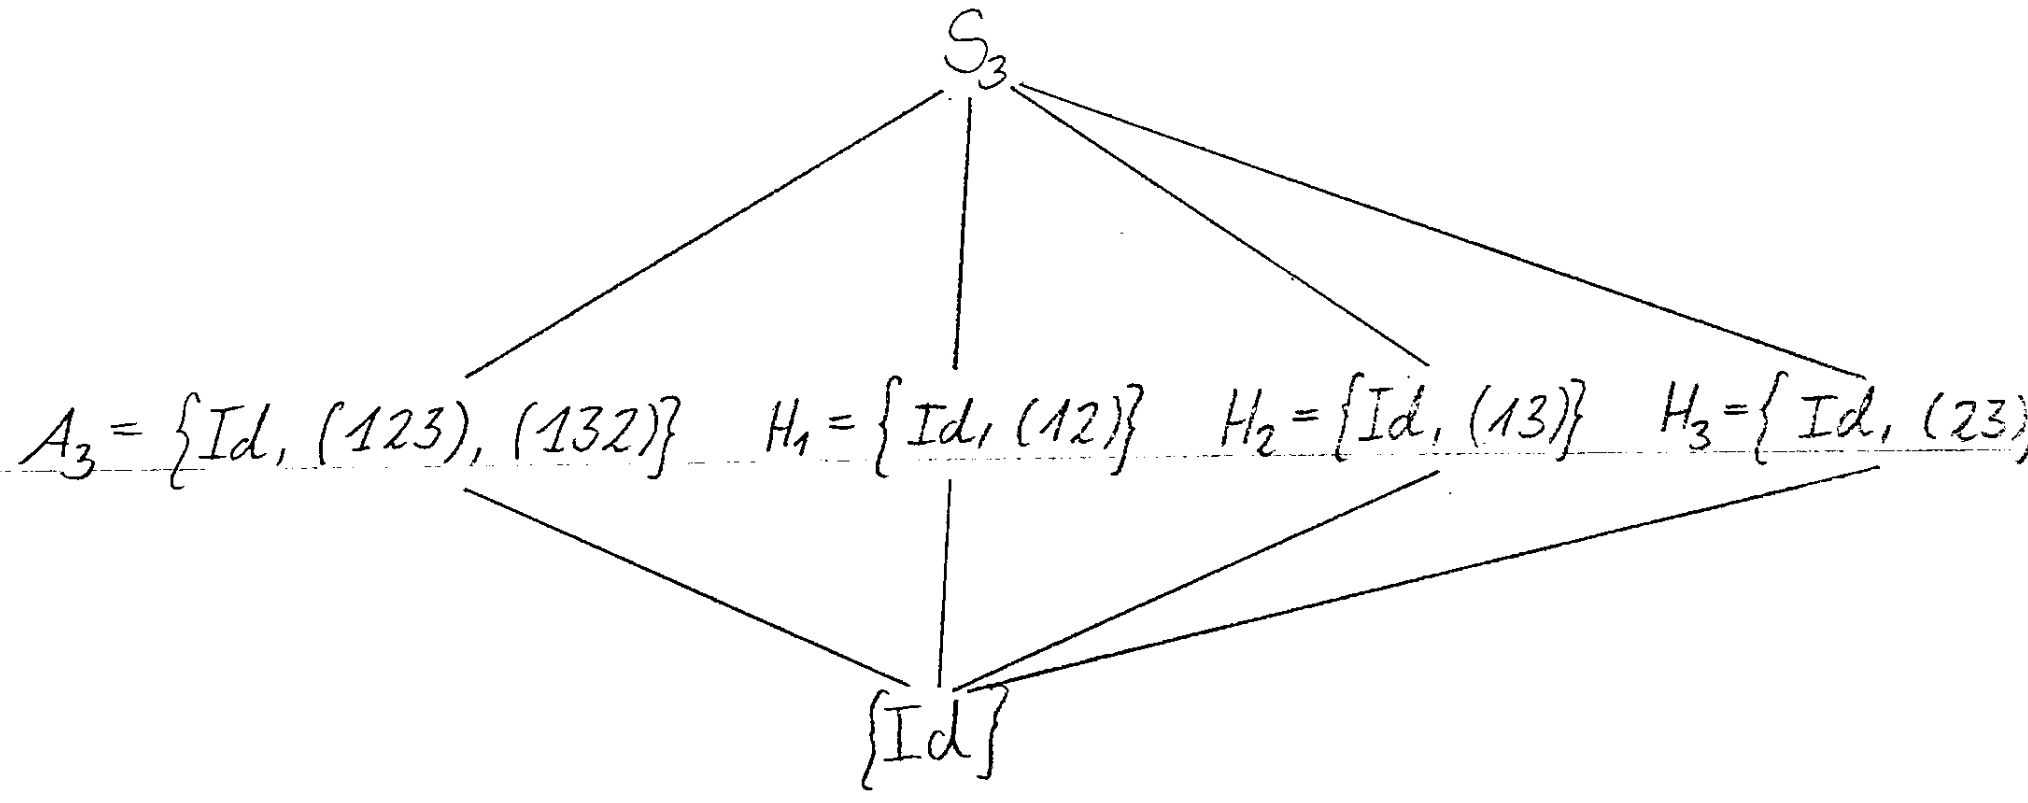
\includegraphics[scale=0.2]{images/beispiel1_15-4}
		%\end{center}
		% https://q.uiver.app/#q=WzAsNixbMywwLCJTXzMiXSxbMCwyLCJBXzMgPSBcXHtcXGlkLCAoMTIzKSwgKDEzMilcXH0iXSxbMiwyLCJIXzEgPSBcXHtcXGlkLCAoMTIpXFx9Il0sWzQsMiwiSF8yID0gXFx7XFxpZCwgKDEzKVxcfSJdLFs2LDIsIkhfMyA9IFxce1xcaWQsICgyMylcXH0iXSxbMyw0LCJcXHtcXGlkXFx9Il0sWzAsMSwiIiwwLHsic3R5bGUiOnsiaGVhZCI6eyJuYW1lIjoibm9uZSJ9fX1dLFswLDIsIiIsMCx7InN0eWxlIjp7ImhlYWQiOnsibmFtZSI6Im5vbmUifX19XSxbMCwzLCIiLDAseyJzdHlsZSI6eyJoZWFkIjp7Im5hbWUiOiJub25lIn19fV0sWzAsNCwiIiwwLHsic3R5bGUiOnsiaGVhZCI6eyJuYW1lIjoibm9uZSJ9fX1dLFsxLDUsIiIsMCx7InN0eWxlIjp7ImhlYWQiOnsibmFtZSI6Im5vbmUifX19XSxbMiw1LCIiLDAseyJzdHlsZSI6eyJoZWFkIjp7Im5hbWUiOiJub25lIn19fV0sWzMsNSwiIiwwLHsic3R5bGUiOnsiaGVhZCI6eyJuYW1lIjoibm9uZSJ9fX1dLFs0LDUsIiIsMCx7InN0eWxlIjp7ImhlYWQiOnsibmFtZSI6Im5vbmUifX19XV0=
		\[\begin{tikzcd}[column sep=tiny]
			&&& {S_3} \\
			\\
			{A_3 = \{\id, (123), (132)\}} && {H_1 = \{\id, (12)\}} && {H_2 = \{\id, (13)\}} && {H_3 = \{\id, (23)\}} \\
			\\
			&&& {\{\id\}}
			\arrow[no head, from=1-4, to=3-1]
			\arrow[no head, from=1-4, to=3-3]
			\arrow[no head, from=1-4, to=3-5]
			\arrow[no head, from=1-4, to=3-7]
			\arrow[no head, from=3-1, to=5-4]
			\arrow[no head, from=3-3, to=5-4]
			\arrow[no head, from=3-5, to=5-4]
			\arrow[no head, from=3-7, to=5-4]
		\end{tikzcd}\]
		
		Es gilt $A_3 \unlhd S_3$. $H_1, H_2, H_3$ sind jedoch keine Normalteiler, da zum Beispiel $(13)H_1(13) = H_3$.
	\end{enumerate}
\end{beispiel}
\begin{satz}\label{satz1_16}
	Sei $G$ eine Gruppe und $H \unlhd G$.
	\begin{enumerate}[label=(\alph*)]
		\item Die Menge $G/H = \{gH \mid g \in G\}$ mit Multiplikation $(aH) \cdot (bH) = (ab)H$ für alle $a,b \in G$ ist eine Gruppe. Sie heißt \textbf{Faktorgruppe} oder \textbf{Quotientengruppe}.
		\item Die Abbildung $\pi \colon G \to G/H$ mit $g \mapsto gH$ ist ein surjektiver Gruppenhomomorphismus mit $\ker(\pi) = H$. $\pi $ heißt \textbf{kanonische Projektion}.
	\end{enumerate}
\end{satz}
\begin{proof}
	\begin{enumerate}[label=(\alph*)]
		\item Die Multiplikation ist wohldefiniert. Sei $aH = a'H$ und $bH = b'H$ bzw. $a^{-1}a' \in H$ und $b^{-1}b' \in H$. 
		
		\underline{Z.z.: $abH = a'b'H$ bzw. $(ab)^{-1} a'b' \in H$.}
		
		\begin{align*}
			(ab)^{-1} a'b' = b^{-1} a^{-1} a' b' = b^{-1} \underbrace{(a^{-1} a')}_{\in H} b \underbrace{(b^{-1} b')}_{\in H} \in H
		\end{align*}
		
		\paragraph{Gruppenaxiome:} 		
		\begin{enumerate}[label={\bfseries(G\arabic*)}]
			\item Multiplikation in $G$ und in $G/H$ assoziativ.
			\item $H$ ist neutrales Element in $G/H$.
			\item Das Inverse zu $gH$ ist $g^{-1}H$.
		\end{enumerate}
		
		\item Für alle $a,b \in G$ gilt 
		\[\pi(ab) = (ab)H = aH \cdot bH = \pi(a)\cdot\pi(b).\]
		Also ist $\pi$ ein Gruppenhomomorphismus mit
		\[\ker(\pi) = \{g \in G \mid gH = H\} = H\]
	\end{enumerate}
\end{proof}
\begin{beispiel}
	Betrachte $n\Z \unlhd \Z$ für $n \in \N$ mit
	\[\faktor{\Z}{n\Z} = \{n\Z, 1 + n\Z, \dots, (n-1) + n\Z\} =: \Z_n,\]
	wobei $(a + n\Z) + (b + n\Z) = (a + b) + n\Z$. Statt $a + n\Z$ schreiben wir auch $\bar{a}$.
	
	Wir können auch Normalteiler in $\Z/n\Z$ betrachten, zum Beispiel
	\[H = \{\bar{0}, \bar{3}\} \unlhd \Z_6.\]
	$H$ ist offensichtlich Untergruppe und auch noch Normalteiler, da $\Z_6$ abelsch ist. Es gilt
	\[\faktor{\Z_6}{H} = \{H, \bar{1} + H, \bar{2} + H\} \cong \Z_3\]
\end{beispiel}

\begin{prop}\label{prop1_18}
	Sei $H \leq G$ eine Untergruppe. Dann gilt $H \unlhd G$ genau dann, wenn $H$ Kern eines Gruppenhomomorphismus ist, der in $G$ startet.
\end{prop}
\begin{proof}
	\glqq{}$\Rightarrow$\grqq: Folgt aus Satz \ref{satz1_16} (b).
	
	\glqq{}$\Leftarrow$\grqq: Sei $\varphi \colon G \to G'$ Gruppenhomomorphismus und $H = \ker(\varphi)$. Nach Beispiel \ref{beispiel1_6} (6) ist $H \leq G$ Untergruppe. Sei nun $g \in G$ und $h \in H$. Dann gilt
	\[\varphi(ghg^{-1}) = \varphi(g) \varphi(h) \varphi(g)^{-1} = \varphi(g) 1_{G'} \varphi(g)^{-1} = 1_{G'}\]
	Es folgt $gHg^{-1} \subseteq H$ und $H \unlhd G$ ist Normalteiler nach Bemerkung \ref{rem1_14}.
\end{proof}
\begin{beispiel}\label{beispiel1_19}
	\begin{enumerate}[label=(\arabic*)]
		\item Nach Beispiel \ref{beispiel1_8} ist $\sgn \colon S_n \to (\{-1,1\}, \cdot)$ für $n > 1$ ein surjektiver Gruppenhomomorphismus. Nach Beispiel \ref{beispiel1_15} (3) gilt
		\[\faktor{S_n}{\ker(\sgn)} = \faktor{S_n}{A_n} = \{A_n, \pi A_n\},\]
		wobei $\sgn(\pi) = -1$. Insbesondere gilt 
		\[\faktor{S_n}{\ker(\sgn)} \cong \Z_2 \cong (\{-1, 1\}, \cdot) = \im(\sgn).\]
		\item Sei $\varphi \colon \R\setminus\{0\}$ mit $x\mapsto |x|$. Dann ist $\varphi$ ein Gruppenhomomorphismus mit $\ker(\varphi) =\{\pm1\}$ und $\im(\varphi) = \R_{>0}$.
		
		Es gilt
		\[\faktor{\R \setminus \{0\}}{\ker(\varphi)} = \faktor{\R \setminus \{0\}}{(\{-1, 1\}, \cdot)} \cong \R_{>0} = \im{\varphi}\]
		
		\item Nach Beispiel \ref{beispiel1_6} (1) ist $\det \colon \GL_n(K) \to K\setminus\{0\}$ ein surjektiver Gruppenhomomorphismus. Es gilt $\ker(\det) = \SL_n(K)$, sowie
		\[\faktor{\GL_n(K)}{\ker(\det)} = \faktor{\GL_n(K)}{\SL_n(K))} \cong K\setminus\{0\} = \im(\det).\]
		Anstatt diesen Isomorphismus explizit nachzuprüfen, beweisen wir
	\end{enumerate}
\end{beispiel}
\begin{satz}[Homomorphiesatz]\label{satz1_20}
	Sei $\varphi \colon G \to H$ ein Gruppenhomomorphismus. Dann gilt
	\[\faktor{G}{\ker(\varphi)} \cong \im(\varphi).\]
	Insbesondere gilt $|G| = |\ker(\varphi)| \cdot |\im(\varphi)|$ für $G$ endlich.
\end{satz}
\begin{proof}
	Betrachte die Abbildung $\bar{\varphi} \colon G/\ker(\varphi) \to \im(\varphi)$ mit $g\ker(\varphi) \mapsto \varphi(g)$. 
	
	$\bar{\varphi}$ ist wohldefiniert, da für $g\ker(\varphi) = g'\ker(\varphi)$ gilt: Es existiert ein $x \in \ker(\varphi)$ mit $g = g'x$ und somit 
	\[\varphi(g) = \varphi(g'x) = \varphi(g')\varphi(x) = \varphi(g') 1_H = \varphi(g')\]
	
	$\bar{\varphi}$ ist Gruppenhomomorphismus, da für $g, g' \in G$ gilt:
	\[\bar{\varphi}(g\ker(\varphi) g'\ker(\varphi)) = \bar{\varphi}(gg'\ker(\varphi)) = \varphi(gg') = \varphi(g) \varphi(g') = \bar{\varphi}(g\ker(\varphi)) \bar{\varphi}(g'\ker(\varphi))\]
	$\bar{\varphi}$ ist nach Konstruktion surjektiv.
	
	$\bar{\varphi}$ ist injektiv, da aus $\bar{\varphi}(g\ker(\varphi)) = \varphi(g) = 1_H$ folgt, dass $g \in \ker(\varphi)$ und somit $g\ker(\varphi) = \ker(\varphi) = 1_{(G/\ker(\varphi))}$ (siehe Beispiel \ref{beispiel1_6} (6)). $\bar{\varphi}$ ist also ein Gruppenisomorphismus, so dass
	\[\faktor{G}{\ker(\varphi)} \cong \im (\varphi).\]
	Für endliche Gruppen $G$ folgt schließlich mit Satz \ref{satz1_11}
	\[|G| = |\ker(\varphi)| \cdot |\im(\varphi)|.\]
\end{proof}

\begin{satz}[Isomorphiesätze]\label{satz1_21}
	Sei $G$ eine Gruppe und $H_1, H_2 \leq G$ Untergruppen.
	\begin{enumerate}[label=(\alph*)]
		\item Ist $H_1 \unlhd G$ Normalteiler, so gilt $H_1H_2 = H_2H_1 \leq G$ und
		\[\faktor{H_1H_2}{H_1} \cong \faktor{H_2}{(H_1 \cap H_2)}.\]
		\item Sind $H_1, H_2 \unlhd G$ Normalteiler mit $H_1 \leq H_2 \leq G$, so gilt
		\[\faktor{G/H_1}{H_2/H_1} \cong \faktor{G}{H_2}\]
	\end{enumerate}
\end{satz}
\begin{proof}
	\begin{enumerate}[label=(\alph*)]
		\item Da $H_1 \unlhd G$, gilt $h_2 H_1 = H_1 h_2$ für alle $h_2 \in H_2$. Somit $H_1H_2 = H_2H_1$. $H_1H_2$ ist Untergruppe, da $1_G \in H_1H_2$ und daher $1_G = 1_G 1_G \in H_1$. Für $h_1, h'_1 \in H$ und $h_2, h'_2 \in H_2$ gilt 
		\[(h_1h_2)(h'_1h'_2) = h_1(\underbrace{h_2h'_1}_{\in H_1H_2}) h'_2 \in H_1 H_2 \]
		Für $h_1 \in H_1, h_2 \in H_2$ gilt $(h_1h_2)^{-1} = h_2^{-1} h_1^{-1} \in H_2 H_1 = H_1 H_2$. Da $H_1 \unlhd G$, gilt auch $H_1 \unlhd H_1H_2$.
		
		Betrachte nun den Homomorphismus
		\begin{center}
			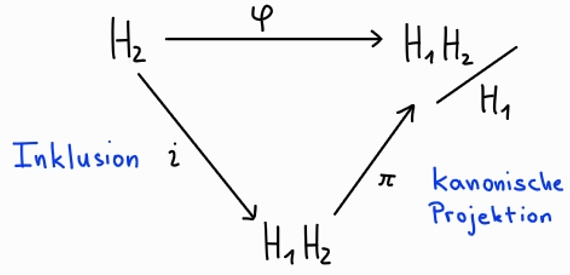
\includegraphics[scale=0.8]{images/2024-10-28_g1}
		\end{center}
		mit $\varphi(h_2) = h_2H_1$. Dann gilt
		\[\ker(\varphi) = \{h_2 \in H_2 \mid h_2 H_1 = H_1\} = H_1 \cap H_2\]
		Da $\varphi$ nach Konstruktion surjektiv, (nutze $H_1 H_2 = H_2 H_1$), folgt mit Satz \ref{satz1_20}
		\[\faktor{H_2}{H_1 \cap H_2} = \faktor{H_2}{\ker(\varphi)} \cong \im(\varphi) = \faktor{H_1H_2}{H_1}.\]
		\item Nach Voraussetzung gilt $H_1 \unlhd H_2$. Die Faktorgruppe $H_2 / H_1$ wird zur Untergruppe von $G/H_1$. Es gilt sogar $H_2/H_1 \unlhd G/H_1$, da für alle $g \in G, h_2 \in H_2$ gilt:
		\[gH_1 h_2H_1 g^{-1} H_1 = \underbrace{gh_2g^{-1}}_{\in H_2, \text{ da } H_2 \unlhd G} H_1.\]
		Betrachte nun den Homomorphismus
		\begin{center}
			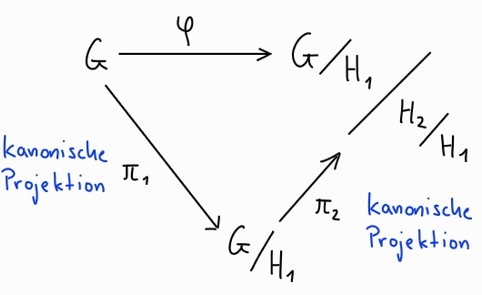
\includegraphics[scale=0.8]{images/2024-10-28_g2}
		\end{center}
		

		mit $\varphi(g) = gH_1(H_2/H_1)$. Dann gilt
		\[\ker(\varphi) = \{g \in G \mid gH_1 \in \faktor{H_2}{H_1}\} = H_2.\]
		Da $\varphi$ nach Konstruktion surjektiv ist (als Komposition surjektiver Abbildungen), folgt wieder mit Satz \ref{satz1_20}:
		\[\faktor{G}{H_2} = \faktor{G}{\ker(\varphi)} \cong \im(\varphi) = \faktor{G/H_1}{H_2 /H_1}.\]
	\end{enumerate}
\end{proof}
\begin{beispiel}
	\begin{enumerate}[label=(\arabic*)]
		\item Sei $G = \Z$, $H_1 = 3\Z \unlhd G$ und $H_2 = 5\Z \unlhd G$. Dann ist $H_1 \cap H_2 = 15\Z$ und $H_1 + H_2 = \Z$, da $1 = 5(-1) + 3 \cdot 2.$ Satz \ref{satz1_21} (a) liefert
		\[\Z_3 = \faktor{\Z}{3\Z} = \faktor{H_1 + H_2}{H_1} \cong \faktor{H_2}{H_1 \cap H_2} = \faktor{5\Z}{15\Z}.\]
		\item Sei $G = \Z$, $H_1 = mn\Z \unlhd G$ und $H_2 = m\Z \unlhd G$ für $m,n \in \N$. Dann liefert Satz \ref{satz1_21} (b)
		\[\Z_m = \faktor{\Z}{m\Z} = \faktor{G}{H_2} \cong \faktor{G/H_1}{H_2/H_1} = \faktor{\Z/mn\Z}{m\Z/mn\Z}.\]
 	\end{enumerate}
\end{beispiel}

Wie sehen Untergruppen von Faktorgruppen aus? Im Beweis von Satz \ref{satz1_21} (b) haben wir verwendet, dass für eine Gruppe $G$ mit $N \unlhd G$ und $N \leq H \leq G$ gilt:
\[\faktor{H}{N} \leq \faktor{G}{N}.\]
Der Beweis zeigt zudem, dass $H \unlhd G \;\Leftrightarrow\; H/N \unlhd G/N$. 

\begin{leftbar}
	{Sind alle Untergruppen von $G/N$ von dieser Form?} -- \textbf{Ja!}
\end{leftbar}

\begin{satz}\label{satz1_23}
	Die Abbildung $\{H \leq G \mid N \leq H\} \to \{\text{Untergruppen von } G/N\}$ mit $H \mapsto H/N$ ist bijektiv.
\end{satz}
\begin{proof}
	Betrachte die kanonische Projektion $\pi \colon G/N$ mit $g \mapsto gN$. Ist $H' \leq G/N$ eine Untergruppe, so gilt 
	\[N \leq \pi^{-1}(H') = \{g \in G \mid \pi(g) \in H'\} \leq G\]
	\begin{itemize}
		\item $g \in N \;\Rightarrow\; \pi(g) = 1_{G/N} \in H'$, also $g \in \pi^{-1}(H')$. Insbesondere $1_G \in \pi^{-1}(H')$.
		\item $g_1, g_2 \in \pi^{-1}(H') \;\Rightarrow\; g_1g_2 \in \pi^{-1}(H')$, da $\pi(g_1g_2) = \underbrace{\pi(g_1)}_{\in H'}\underbrace{\pi(g_2)}_{\in H'} \in H'$.
		\item $g \in \pi^{-1}(H') \;\Rightarrow\; g^{-1} \in \pi^{-1}(H')$, da $\pi(g^{-1}) = \pi(g)^{-1} \in H'$.
	\end{itemize}
	Die Umkehrabbildung zur gegebenen Abbildung in der Aussage liefert die Zuordnung $H' \mapsto \pi^{-1}(H')$, da 
	\[\faktor{\pi^{-1}(H')}{N} = H' \quad\text{sowie}\quad \pi^{-1}(H/N) = H\]
\end{proof}

\begin{rem}\label{rem1_24}
	Die Bijektion in Satz \ref{satz1_23} ist inklusionserhaltend und zeigt, dass die kanonische Projektion $\pi \colon G \to G/N$ einen Isomorphismus von Untergruppenverbänden induziert:
	\begin{center}
		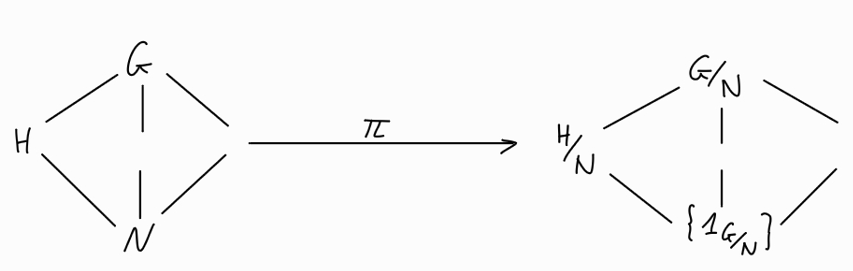
\includegraphics[scale=0.8]{images/2024-10-28_g3}
	\end{center}
\end{rem}
	
	% Endlich erzeugte Gruppen
	\section{Endlich erzeugte Gruppen}

\begin{definition}
	Sei $G$ eine Gruppe und $S \subseteq G$ eine Teilmenge. Definiere 
	\[\langle S \rangle := \bigcap_{H \leq G, S \subseteq H} H \leq G.\]
	$\langle S \rangle$ heißt \textbf{die von $S$ erzeugte Untergruppe} von $G$.
\end{definition}
Falls $G = \langle S \rangle$, so heißt $S$ \textbf{Erzeugendensystem} von $G$. Hat $G$ ein endliches Erzeugendensystem, so heißt $G$ \textbf{endlich erzeugt}. Gibt es ein $g \in G$ mit $G = \langle \{g\} \rangle =: \langle g \rangle$, so heißt $G$ \textbf{zyklisch}.
\begin{rem}
	\begin{enumerate}[label=(\roman*)]
		\item Nach Konstruktion ist $\langle S\rangle$ die kleinste Untergruppe von $G$, die $S$ enthält.
		\item Für $S \neq \emptyset$ ist $\spn{S} = \{s_1 \cdots s_t \mid t \in \N, s_i \in S \cup S^{-1}\}$. 
		
		Insbesondere ist für $g \in G$:
		\[\spn{g} = \{g^n \mid n \in \Z\} \quad\text{mit}\quad g^n := \begin{cases}
			1_G, & n = 0\\
			\underbrace{g \cdots g}_{n-\text{mal}}, & n > 0\\
			\underbrace{g^{-1} \cdots g^{-1}}_{(-n)-\text{mal}}, & n < 0 
		\end{cases}\]
\end{enumerate}
\begin{leftbar}
	Wir wollen zunächst zyklische Gruppen besser verstehen!
\end{leftbar}
\end{rem}
\begin{beispiel}\label{beispiel2_3}
	\begin{enumerate}[label=(\arabic*)]
		\item $(\Z, +) = \spn{1} = \spn{-1}$ ist eine zyklische Gruppe.
		
		$(\Z_m, +) = \spn{\bar{1}}$ ist eine zyklische Gruppe der Ordnung $m$.
		
		\item Sei $G$ eine Gruppe mit $|G| = p$ Primzahl. Dann ist $G$ zyklisch.
		\begin{proof}
			Sei $1_G \neq g \in G$ und betrachte $\spn{g} \leq G$. Nach Satz \ref{satz1_11} $|\spn{g}|$ teilt $|G| = p$. Da $\spn{g} > 1$ nach Voraussetzung folgt $|\spn{g}| = p$. Somit $G = \spn{g}$.
		\end{proof}
	\end{enumerate}
\end{beispiel}
\begin{satz}\label{satz2_4}
	\begin{enumerate}[label=(\alph*)]
		\item Eine Gruppe $G$ ist zyklisch genau dann, wenn es einen surjektiven Gruppenhomomorphismus von der Form $\Z \to G$ gibt.
		\item Für eine zyklische Gruppe $G$ gilt:
		\[G \cong \begin{cases}
			\Z, & |G| = \infty,\\
			\Z_m, & |G| = m.
		\end{cases}\]
		Zudem ist jede Untergruppe von $G$ wieder zyklisch.
	\end{enumerate}
\end{satz}
\begin{proof}
	\begin{enumerate}[label=(\alph*)]
		\item \glqq{}$\Rightarrow$\grqq: Sei $G = \spn{g} = \{g^n \mid n \in \Z\}$. Definiere einen Gruppenhomomorphismus $\Z \to G$ durch $m \mapsto g^n$. Dieser ist nach Voraussetzung surjektiv.
		
		\glqq{}$\Leftarrow$\grqq: Sei $\varphi \colon \Z \to G$ ein surjektiver Gruppenhomomorphismus. Definiere $g := \varphi(1) \in G$.
		
		\underline{Behauptung}: $G = \spn{g}$.
		
		Die Inklusion $\spn{g} \subseteq G$ ist klar. Sei nun $h \in G$ beliebig. Da $\varphi$ surjektiv ist, existiert $n \in \Z$ mit $\varphi(n) = h$. Da $\varphi$ Gruppenhomomorphismus, gilt
		\[h = \varphi(n) = \begin{cases}
			\underbrace{\varphi(1) \cdots \varphi(1)}_{n-\text{mal}}, & n \geq 0\\
			\underbrace{\varphi(1)^{-1} \cdots \varphi(1)^{-1}}_{n-\text{mal}}, &n < 0
		\end{cases}\]
		Daraus folgt $h = g^n \in \spn{g}$.
		
		\item Sei $G$ zyklisch und $\varphi \colon \Z \to G$ ein surjektiver Gruppenhomomorphismus, der nach (a) existiert. Nach Satz \ref{satz1_20} gilt
		\[G \cong \faktor{\Z}{\ker(\varphi)}.\]
		Nach Aufgabe M.1.4. wissen wir, dass $\ker(\varphi) = m\Z$ für ein $m \in \N_0$. Damit folgt der erste Teil der Behauptung.
		
		Sei nun $H \leq G$. Dann ist $\varphi^{-1}(H)$ eine Untergruppe von $\Z$ (siehe Beweis zu Satz \ref{satz1_23}) und somit erneut $\varphi^{-1}(H) = m\Z, \; m \in\N_0$. Insbesondere ist $\varphi^{-1}(H) = \spn{m} \leq \Z$. Da $\varphi$ surjektiv ist, gilt $\varphi(\varphi^{-1}(H)) = H$ und $H$ wird von $\varphi(n)$ erzeugt.
	\end{enumerate}
\end{proof}
\begin{definition}
	Sei $G$ eine Gruppe und $g \in G$. Die \textbf{Ordnung von $g$} ist definiert als die Ordnung $\spn{g}$, der von $g$ erzeugten zyklischen Untergruppe von $G$.
	
	Wir schreiben $\ord(g)$ für die Ordnung von $g$. 
\end{definition}
\begin{rem}
	Ist $\ord(g) = m \in \N$ bzw. $\spn{g} \cong \Z_m$ mit $\spn{g} = \{1_G, g, \dots, g^{m-1}\}$ nach Satz \ref{satz2_4} (b), so gilt $g^n = 1_G$ genau dann, wenn $n \in m\Z$. 
	
	Ist $G$ endlich, so gilt $\ord(g)$ teilt $|G|$ nach Satz \ref{satz1_11} und somit $g^{|G|} = 1_G$ (\textbf{Kleiner Fermat'scher Satz}).
	
	Ist $\ord(g) = \infty$ bzw. $\spn{g} \cong \Z$, so sind die $g^n$ mit $n \in \Z$ paarweise verschieden.
\end{rem}
\begin{beispiel}
	\begin{enumerate}[label=(\arabic*)]
		\item Für $\bar{a} \in \Z_m$ mit $m \in \N$ gilt $\ord(\bar{a}) = \frac{m}{\ggt(a,m)}$. Zum Beispiel hat $\bar{8} \in \Z_{12}$ die Ordnung $\frac{12}{\ggt(8,12)} = \frac{12}{4} = 3$.
		
		\item Für $n \geq 3$ sei $D_n$ die Symmetriegruppe eines regelmäßigen $n$-Ecks in $\R^2$. Diese heißt auch \textbf{Diedergruppe}. Für $n = 3$ gilt $D_3 \cong S_3$.
		
		Im Allgemeinen enthält $D_n$ genau $n$ Drehungen und $n$ Spiegelungen, so dass $|D_n| = 2n$. Sei $r$ eine Drehung um $\frac{2\pi}{n}$ und $s$ eine beliebige Spiegelung. Dann gilt $\ord(r) = n$ und $\ord(s) = 2$, sowie $D_n = \{\id, r, r^2, \dots, r^{n-1}, s, sr, sr^2, \dots, sr^{n-1}\} = \spn{\{r,s\}}$.
	\end{enumerate}
\end{beispiel}

\begin{center}
	\textit{Welche Gruppen können wir aus zyklischen Gruppen zusammensetzen?}
\end{center}

\begin{definition}
	Eine Gruppe $G$ heißt \textbf{inneres direktes Produkt} von $G_1$ und $G_2$, falls
	\begin{itemize}
		\item $G_1, G_2 \unlhd G$.
		\item $G_1 \cdot G_2 = G$.
		\item $G_1 \cap G_2 = \{1_G\}$.
	\end{itemize}
\end{definition}

\begin{rem}
	\begin{enumerate}[label=(\roman*)]\label{rem2_9}
		\item Ist $G = G_1 \times G_2$ (äußeres) direktes Produkt der Gruppen $G_1$ und $G_2$, so ist $G$ inneres direktes Produkt von $G_1 \times \{1_G\}$ und $\{1_G\} \times G_2$.
		
		\item Ist $G$ inneres direktes Produkt von $G_1$ und $G_2$, so gilt
		\[G \cong G_1 \times G_2.\]
		\begin{proof}
			Betrachte die Abbildung $\varphi \colon G_1 \times G_2$ mit $(g_1, g_2) \mapsto g_1g_2$. Da $\underbrace{g_1g_2g_1^{-1}}_{\in G_2}  g_2^{-1} = g_1(\underbrace{g_2g_1^{-1}g_2^{-1}}_{\in G_1}) \in G_1 \cap G_2 = \{1_G\}$, folgt $g_1 = g_2$. Somit gilt $\varphi((g_1, g_2) (h_1, h_2)) = \varphi(g_1h_1, g_2h_2) = g_1(h_1g_2)h_2 = (g_1g_2)(h_1h_2) = \varphi((g_1, g_2)) \varphi((h_1, h_2))$. $\varphi$ ist zudem bijektiv nach Voraussetzung.
		\end{proof}
	\end{enumerate}
\end{rem}
\begin{beispiel}
	\begin{enumerate}[label=(\arabic*)]
		\item Die abelsche Gruppe $\C \setminus \{0\}$ ist inneres direktes Produkt von $\R_{>0}$ und $S^1 := \{z \in \C \mid |z| = 1\}$.
		\item Nach Aufgabe S.2.2. gilt 
		\[V_4 = \{\id, (12)(34), (13)(24), (14)(23)\} \unlhd S_4\]
		mit $S_4/V_4 \cong S_3$. Die $S_3$ ist isomorph zu einer Untergruppe $H$ von $S_4$ (Beispiel \ref{beispiel1_6} (4)), so dass $V_4 \cdot H = S_4$ und $V_4 \cap H = \{\id\}$. Aber $S_4$ ist nicht inneres direktes Produkt von $V_4$ und $H$, da $H$ kein Normalteiler von $S_4$.
	\end{enumerate}
\end{beispiel}
\begin{thm}\label{thm2_11}
	Jede endlich erzeugte abelsche Gruppe ist ein endliches inneres direktes Produkt zyklischer Gruppen.
\end{thm}
\begin{proof}
	Sei $(G, +)$ abelsche Gruppe, erzeugt von $S = \{a_1, \dots, a_k\} \subseteq G$. 
	
	\textbf{Induktion über $k$:} Für $k = 1$ ist $G$ zyklisch.
	
	Betrachte den surjektiven Gruppenhomomorphismus
	\[\varphi_S \colon \Z^k \to G \quad\text{mit}\quad(n_1, \dots, n_k) \mapsto n_1a_1 + \dots + n_ka_k.\]
	Sei $\pi \colon \Z^k \to \Z$ die Projektion auf die erste Komponente, also
	\[\pi((n_1, \dots, n_k)) = n_1.\]
	Das Bild von $\ker(\varphi_S)$ unter $\pi$ ist Untergruppe von $\Z$ und somit von der Form $d\Z$ für $d \in \N_0$. Sei o.B.d.A. $S$ so gewählt, dass $d$ minimal ist. Falls $d = 0$, so ist $\spn{a_1} \cap \spn{S\setminus\{a_1\}}= \{0_G\}$ und $\ord{a_1} = \infty$, d.h. $G$ ist inneres direktes Produkt von $\spn{a_1}$ und $\spn{S\setminus\{a_1\}}$, wobei $\spn{a_1} \cong \Z$.
	
	Auf $S\setminus\{a_1\}$ können wir die Induktionsvoraussetzung anwenden. 
	
	Falls $d > 0$, wähle $(n_1, \dots, n_k) \in \ker(\varphi_S)$ mit $n_1 = d$. Sei $2 \leq i \leq k$. Division mit Rest liefert $q_i, d_i \in \Z$ mit
	\[n_i = q_i d + d_i \quad\text{und}\quad 0 \leq d_i < d.\]
	Definiere $S_i := \{b_1, \dots, b_k\}$ durch $b_1 = a_i$ und $b_i = a_1 + q_i a_i$ und $b_j = a_j$ sonst. Dann ist auch $S_i$ Erzeugendensystem von $G$. Zudem liegt der Vektor
	\[(d_i, n_2, \dots, i, \dots, n_k) \in \Z^k\]
	im Kern von $\varphi_{S_i}$, da
	\[d_ib_1 + db_i = (n_i - q_id)a_i + d(a_1 + q_ia_i) = n_ia_i + n_1a_1\]
	und weil $(n_1, \dots, n_k) \in \ker(\varphi_S)$. Wegen der Minimalität von $d$ ist $1 \leq d_i < d$ ausgeschlossen, d.h.
	\[d_i = 0 \quad\text{und}\quad d \big| n_i.\]
	Setze nun $x_i = \frac{n_i}{d}$ für $1 \leq i \leq k$. Insbesondere $x_1 = 1$. Dann wird $G$ von der Menge
	\[\bigg\{\underbrace{\sum_{i=1}^k x_ia_i}_{=: a} , a_2, \dots, a_k\bigg\}\]
	mit $\spn{a} \cap \spn{\{a_2, \dots, a_k\}} = \{0_G\}$. Denn ein Element im Schnitt hat die Form 
	\[m_1a = \sum_{i=2}^k m_ia_i\]
	für $(m_1, \dots, m_k) \in \Z^k$, so dass $m_1$ im Bild von $\ker(\varphi_S)$ unter $\pi$ liegt, also ein Vielfaches von $d$ ist. Es gilt aber bereits
	\[da = n_1 a_1 + \dots + n_ka_k = 0_G.\]
	Somit ist $G$ inneres direktes Produkt von $\spn{a}$ und $\spn{S \setminus \{a_1\}}$, wobei  $\spn{a} \cong \Z_d$. Nun können wir erneut die Induktionsvoraussetzung anwenden.
\end{proof}
\begin{kor}[Hauptsatz für endlich erzeugte abelsche Gruppen]\label{kor2_12}
	Sei $G$ eine endlich erzeugte Gruppe. Dann existieren eindeutige $r,t \in \N_0$ sowie bis auf Reihenfolge eindeutig bestimmte Primzahlpotenzen 
	\[1 < p_1^{k_1} \leq \dots \leq p_t^{k_t} \quad\text{mit}\quad G \cong \Z^r \times \Z_{p_1^{k_1}} \times \dots \times \Z_{p_t^{k_t}}.\]
\end{kor}
\begin{proof}
	Die Existenz folgt aus Theorem \ref{thm2_11} zusammen mit Bemerkung \ref{rem2_9} (ii) und Aufgabe M.3.3. Letztere besagt, dass für $m, n \in \N$ mit $\mathrm{ggT}(m,n) = 1$ gilt $\Z_{nm} \cong \Z_n \times \Z_m$. Die Eindeutigkeit können/wollen wir hier nicht beweisen.
\end{proof}
Was können wir im nicht-abelschen Fall tun? Eine Klassifikation aller endlich erzeugten oder endlichen Gruppen ist hoffnungslos. Im Jahr 1982 hat man die Klassifikation aller endlichen einfachen Gruppen abgeschlossen, also aller endlichen Gruppen mit genau zwei (trivialen) Normalteilern. Dies war ein Mammutprojekt!
\begin{itemize}
	\item mehr als 500 Fachartikel,
	\item mehr als 100 MathematikerInnen,
	\item Zeitraum von über 50 Jahren,
	\item Einsatz von Computern.
\end{itemize}
Die endlichen einfachen Gruppen sind von der Form
\begin{enumerate}[label=(\arabic*)]
	\item Zyklische Gruppe $\Z_p$ mit $p$ Primzahl.
	\item Alternierende Gruppen $A_n$ für $n \geq 5$.
	\item Endliche Gruppen vom Lie-Typ, z.B.
	\[\mathsf{PSL}_(K) := \faktor{\SL_n(K)}{Z(\SL_n(K))} = \faktor{\SL_n(K)}{\{\lambda E_n \mid \lambda^n = 1\}}\]
	für $n > 2$ und einen endlichen Körper $K$.
	\item 26 sporadische Gruppen mit bis zu ungefähr $8 \cdot 10^{53}$ Elementen, die sogenannten Monster!
\end{enumerate}
\begin{beispiel}\label{beispiel2_13}
	Die alternierende Gruppe $A_4$ ist nicht einfach nach Aufgabe S.2.2. Aber für $n \geq 5$ ist $A_n$ einfach.
\end{beispiel}
\begin{proof}
	Sei $\{\id\} \neq N \unlhd A_n$. Wir zeigen, dass $N = A_n$. 
	
	\textbf{Schritt 1: } $N$ enthält einen Zykel der Länge 3. 
	
	Sei $\id \neq \sigma \in N$. Ist $\sigma$ kein Zykel der Länge 3, so gilt einer der folgenden Fälle:
	\begin{enumerate}[label=(\roman*)]
		\item $\sigma = (a_1 a_2 a_3 a_4 \dots)\dots$
		\item $\sigma = (a_1 a_2 a_3)(a_4 a_5 a_6)\dots$
		\item $\sigma = (a_1 a_2)(a_3 a_4)(a_5 a_6)\dots$
		\item $\sigma = (a_1 a_2)(a_3 a_4)$
	\end{enumerate}
	Da $N$ Normalteiler ist, gilt $(\pi \sigma \pi^{-1})\sigma^{-1} \in N$ für alle $\pi \in A_n$. Im Fall (i) wähle $\pi = (a_2 a_1 a_3)$.
	\[(\pi \sigma \pi^{-1})\sigma^{-1} = (a_2 a_1 a_3)\sigma(a_1 a_2 a_3)\sigma^{-1} = (a_1 a_3 a_4).\]
	Im Fall (ii) wähle $\pi = (a_3 a_2 a_4)$.
	\[(\pi\sigma\pi^{-1})\sigma^{-1} = (a_3 a_2 a_4)\sigma(a_2a_3a_4)\sigma^{-1} = (a_1 a_5 a_2 a_4 a_3)\]
	und weiter im Fall (i). Im Fall (iii) wähle $\pi = (a_2 a_1 a_3)$:
	\[(\pi\sigma\pi^{-1}) \sigma^{-1} = (a_2 a_1 a_3)\sigma(a_1 a_2 a_3) \sigma^{-1} = (a_1 a_4)(a_2 a_3).\]
	Im Fall (iv) wähle $\pi = (a_2 a_1 a_5)$:
	\[(\pi\sigma\pi^{-1})\sigma^{-1} = (a_2 a_1 a_5)\sigma(a_1 a_2 a_5)\sigma^{-1} = (a_1 a_2 a_5).\]
	Also enthält $N$ einen Zykel der Länge 3.
	
	\textbf{Schritt 2: } $N = A_n$.
	
	Sei $(a_1 a_2 a_3) \in N$. Da $N \unlhd A_n$ ist, gilt:
	\[(a_3 a_4 a_5)(a_1 a_2 a_3)(a_4 a_3 a_5) = (a_1 a_2 a_4) \in N.\]
	Insbesondere sind alle Zykel der Form $(a_1 a_2 x)$ in $N$ mit $x \in \{1,\dots, n\} \setminus \{a_1, a_2\}$. Wiederholen des Arguments zeigt, dass alle Zykel der Länge 3 in $N$ enthalten sind. Da $A_n$ nach Aufgabe M.3.2. von diesen Zykeln erzeugt wird, folgt $N = A_n$.
\end{proof}
\begin{leftbar}
	{Warum sind endliche einfache Gruppen so wichtig?}
\end{leftbar}

\begin{definition}
	Sei $G$ ein Gruppe. Eine Folge von Untergruppen
	\[\{1_G\} = G_0 \unlhd G_1 \unlhd G_2 \unlhd \dots \unlhd G_n = G\]
	heißt \textbf{Normalreihe der Länge $n$}. Die Faktoren $G_i/G_{i-1}$ heißen \textbf{Faktoren} der Normalreihe. Eine Normalreihe von $G$ heißt \textbf{Kompositionsreihe}, falls alle ihre Faktoren einfach sind. Die Faktoren einer Kompositionsreihe heißen \textbf{Kompositionsfaktoren}.
\end{definition}
\begin{rem}\label{rem2_15}
	\begin{enumerate}[label=(\roman*)]
		\item Jede Gruppe $G$ hat die Normalreihe $\{1_G\} \unlhd G$.
		\item Jede endliche Gruppe $G$ hat eine Kompositionsreihe.
		
		Induktion nach $|G|$. Ist $G$ einfach, dann ist $\{1_G\} \unlhd G$ Kompositionsreihe. Ist andernfalls $N \unlhd G$ maximaler echter Normalteiler. nach Satz \ref{satz1_23} ist $G/N$ einfach und $N$ hat nach Induktionsvoraussetzung eine Kompositionsreihe
		\[\{1_G\} = N_0 \unlhd N_1 \unlhd \dots \unlhd N_t = N.\]
		Dann ist $\{1_G\} = N_0 \unlhd N_1 \unlhd \dots \unlhd N_t = N \unlhd G$ eine Kompositionsreihe von $G$.
		
		\item Die Gruppe $\Z$ hat keine Kompositionsreihe (nutze Klassifikation der Untergruppen von $\Z$).
	\end{enumerate}
\end{rem}
\begin{thm}\label{Satz von Jordan-Hölder}
	Sei $G$ eine endliche Gruppe. Dann alle Kompositionsreihen von $G$ \textbf{äquivalent}, das heißt sie haben die selbe Länge und bis auf Isomorphie und Reihenfolge die selben Kompositionsfaktoren.
\end{thm}
\begin{proof}
	Betrachte die folgenden Kompositionsreihen:
	\begin{enumerate}[label=(\Roman*)]
		\item $\{1_G\} = G_0 \unlhd G_1 \unlhd \dots \unlhd G_r = G$,
		\item $\{1_G\} = H_0 \unlhd H_1 \unlhd \dots \unlhd H_s = G$.
	\end{enumerate}
	\textbf{Induktion nach $r$: } Für $r = 1$ ist $G$ einfach. Also auch $G = H_1$.
	
	Sei $r > 1$. 
	
	\textbf{Fall 1: } $G_{r-1} = H_{s-1}$. Dann hat $G_{r-1}$ die Kompositionsreihen $\{1_G\} = G_0 \unlhd \dots \unlhd G_{r-1}$ und $\{1_G\} = H_0 \unlhd \dots \unlhd H_{s-1} = G_{r-1}$. Nach Induktionsvoraussetzung sind diese beiden und somit auch die ursprünglichen beiden Kompositionsreihen \textbf{(I)} und \textbf{(II)} von $G$ äquivalent.
	
	\textbf{Fall 2: } $G_{r-1} \neq H_{s-1}$. Betrachte $G_{r-1} \unlhd G_{r-1}\dots H_{s-1} \unlhd G$. Da $G_{r-1} \neq H_{s-1}$ und $G_r / G_{r-1}$ und $G/H_{s-1}$ einfach, folgt mit Satz \ref{satz1_23}, dass $G_{r-1}H_{s-1} = G$. Sei $J = G_{r-1} \cap H_{s-1}$ mit $J \unlhd G$. Nach Satz \ref{satz1_21} (a) gilt
	\[\faktor{G}{G_{r-1}} = \faktor{G_{r-1}H_{s-1}}{G_{r-1}} \cong \faktor{H_{s-1}}{J}\]
	sowie 
	\[\faktor{G}{H_{s-1}} = \faktor{H_{s-1} G_{r-1}}{H_{s-1}} \cong \faktor{G_{r-1}}{J}\]
	d.h. $H_{s-1} / J$ und $G_{r-1}/J$ sind einfach. Nach Bemerkung \ref{rem2_15} (ii) hat $J$ eine Kompositionsreihe
	\[\{1_G\} = J_0 \unlhd J_1 \unlhd \dots \unlhd J_t = J.\]
	Diese induziert die folgenden beiden Kompositionsreihen von $G$:
	\begin{enumerate}[start=3,label=(\Roman*)]
		\item $\{1_G\} = J_0 \unlhd \dots \unlhd J_t = J \unlhd G_{r-1} \unlhd G$,
		\item $\{1_G\} = J_0 \unlhd \dots \unlhd J_t = J \unlhd H_{s-1} \unlhd G$.
	\end{enumerate}
	Diese sind äquivalent, da bis auf Isomorphie nur die letzten beiden Faktoren vertauscht werden. Nach Induktionsvoraussetzung sind auch die Kompositionsreihen \textbf{(I)} und \textbf{(III)} von $G$ äquivalent. Insbesondere gilt $r-1 = t+1$. Somit liefert \textbf{(IV)} eine Kompositionsreihe von $H_{s-1}$ der Länge $r-1$, die nach Induktionsvoraussetzung äquivalent ist zu $\{1_G\} = H_0 \unlhd \dots \unlhd H_{s-1}$. Folglich sind auch die Kompositionsreihen \textbf{(II)} und \textbf{(IV)} äquivalent. Dies liefert die gewünschte Äquivalenz von \textbf{(I)} und \textbf{(II)}.
\end{proof}
\begin{beispiel}
	$\Z_6$ hat die Kompositionsreihen $\{\bar{0}\} \unlhd \spn{\bar{2}} \unlhd \Z_6$ und $\{\bar{0}\} \unlhd \spn{\bar{3}} \leq \Z_6$ mit Kompositionsfaktoren isomorph zu $\Z_2$ und $\Z_3$.
	
	Die symmetrische Gruppe $S_3$ hat die Kompositionsreihe $\{\id\} \unlhd A_3 \unlhd S_3$, deren Kompositionsfaktoren auch isomorph zu $\Z_2$ und $\Z_3$ sind. Aber $\Z_6 \cong \Z_2 \times \Z_3 \not\cong S_3$!
\end{beispiel}
% Vorlesung vom 11.11.2024:
Wir haben gesehen, dass sich endliche abelsche Gruppen, auf im Wesentlichen, eindeutige Art und Weise, aus einfachen Gruppen zusammenkleben lassen. Aber welche Gruppen können wir aus einfachen zyklischen Gruppen zusammenkleben?
\begin{definition}
	Eine Gruppe $G$ heißt \textbf{auflösbar}, wenn $G$ eine Normalreihe mit abelschen Faktoren hat, d.h. es gibt eine Folge von Untergruppen
	\[\{1_G\} = G_0 \unlhd G_1 \unlhd \dots \unlhd G_n = G\]
	mit $G_i/G_{i-1}$ abelsch für alle $1 \leq i \leq n$.
\end{definition}
\begin{rem}
	Auflösbare Gruppen werden uns in der Algebra II helfen zu entscheiden, ob Gleichungen durch endliche Wurzelausdrücke aufgelöst werden können (siehe Kapitel 0).
\end{rem}
\begin{beispiel}\label{beispiel2_20}
	\begin{enumerate}[label=(\arabic*)]
		\item Abelsche Gruppen sind auflösbar. Nach Theorem \ref{thm2_11} bzw. \ref{kor2_12} wissen wir, dass wir endliche abelsche Gruppen aus einfachen zyklischen Gruppen zusammenkleben können.
		\item Jede einfache auflösbare Gruppe $G$ ist isomorph zu $\Z_p$, $p$ prim.
		\begin{proof}
			Da $G$ einfach, existiert nur die triviale Normalreihe $\{1_G\} \unlhd G$. Da $G$ auflösbar ist, folgt, dass $G$ abelsch ist und abelsche Gruppen ohne echten Normalteiler sind isomorph zu $\Z_p$.
		\end{proof}
		\item Die alternierende Gruppe $A_n$ mit $n \in \N$ ist auflösbar genau dann, wenn $n \leq 4$.
		\begin{proof}
			Für $n \leq 3$ ist $A_n$ abelsch und dadurch auflösbar. Für $n = 4$ betrachte die Normalreihe $\{1_G\} \unlhd V_4 \unlhd A_4$ mit Faktoren $V_4 \cong \Z_2 \times \Z_2$ und $A_4 / V_4 \cong \Z_3$ (siehe Aufgabe S.2.2.). Für $n \geq 5$ nutze Beispiel \ref{beispiel2_13}.
		\end{proof}
		\item Man kann zeigen, dass endliche Gruppen ungerader Ordnung auflösbar stets auflösbar sind. (\textbf{Satz von Feit-Thompson} (1963))
		\item Die kleinste nicht auflösbare Gruppe ist die $A_5$.
	\end{enumerate}
\end{beispiel}
\begin{prop}\label{prop2_21}
	Sei $G$ eine auflösbare Gruppe.
	\begin{enumerate}[label=(\alph*)]
		\item Jede Untergruppe von $H \leq G$ ist auflösbar.
		\item Ist $N \unlhd G$ Normalteiler, so ist auch $G/N$ auflösbar. 
	\end{enumerate}
\end{prop}
\begin{proof}
	Sei $\{1_G\} = G_0 \unlhd G_1 \unlhd \dots \unlhd G_n = G$ eine Normalreihe von $G$ mit der Eigenschaft $G_i/G_{i-1}$ abelsch für alle $i \in \{1, \dots, n\}$.
	\begin{enumerate}[label=(\alph*)]
		\item Betrachte die induzierte Normalreihe der Form
		\[\{1_G\} = G_0 \cap H \unlhd G_1 \cap H \unlhd \dots \unlhd G_n \cap H = H.\]
		Nach Satz \ref{satz1_21} (a) gilt für alle $i \in \{1, \dots, n\}$
		\[\faktor{G_i \cap H}{G_{i-1} \cap H} = \faktor{G_i \cap H}{G_{i-1} \cap G_i \cap H} \cong \faktor{G_{i-1} \cdot (G_i \cap H)}{G_{i-1}} \leq \faktor{G_i}{G_{i-1}}\]
		Da $G_i / G_{i-1}$ abelsch ist, so ist auch $(G_i \cap H) / (G_{i-1}\cap H)$ abelsch. Somit ist $H$ auflösbar.
		
		\item Betrachte die durch die kanonische Projektion $\pi \colon G \to G/N$ induzierte Normalreihe der Form $\{1_{G/N}\} = \pi(G_0) \unlhd \pi(G_1) \unlhd \dots \unlhd \pi(G_n) = G/N$. Für $i \in \{1, \dots, n\}$ erhalten wir einen surjektiven Gruppenhomomorphismus 
		\[\varphi \colon G_i \to \faktor{\pi(G_i)}{\pi(G_{i-1})}\]
		durch $g_i \mapsto \pi(g_i)\pi(G_{i-1})$ mit 
		\[G_{i-1} \unlhd \ker(\varphi) \unlhd G_i.\]
		Nach Satz \ref{satz1_20} und Satz \ref{satz1_21} (b) gilt
		\[\faktor{\pi(G_i)}{\pi(G_{i-1})} \cong \faktor{G_i}{\ker(\varphi)} \cong \faktor{G_i / G_{i-1}}{\ker(\varphi) / G_{i-1}}.\]
		Da $G_i / G_{i-1}$ abelsch ist, so sind auch deren Quotienten abelsch und somit insbesondere $\pi(G_i) / \pi(G_{i-1})$. Also ist $G/N$ auflösbar.
	\end{enumerate}
\end{proof}
\begin{satz}\label{satz2_22}
	Sei $G$ eine Gruppe mit Kompositionsreihe. Dann ist $G$ auflösbar genau dann, wenn alle Kompositionsfaktoren von $G$ isomorph zu $\Z_p$ für $p$ Primzahl.
\end{satz}
\begin{proof}
	\glqq{}$\Leftarrow$\grqq: Folgt unmittelbar, da $\Z_p$ abelsch ist.
	
	\glqq{}$\Rightarrow$\grqq: Sei $G_i / G_{i-1}$ ein Kompositionsfaktor von $G$ mit $G_{i-1} \unlhd G_i \leq G$. Da $G$ auflösbar ist, sind nach Proposition \ref{prop2_21} sowohl $G_i$ als auch $G_i / G_{i-1}$ auflösbar. Da $G_i / G_{i-1}$ zudem einfach ist, folgt die Behauptung mit Beispiel \ref{beispiel2_20} (2).
\end{proof}





	
	% Gruppenwirkungen
	\section{Operationen von Gruppen auf Mengen}
\begin{definition}
	Sei $G$ eine Gruppe und $X \neq \emptyset$ eine Menge. Dann heißt $X$ \textbf{$G$-Menge}, wenn es eine Abbildung $* \colon G \times X \to X$, $(g,x) \mapsto g*x$ gibt mit 
		\begin{enumerate}[label={\bfseries(O\arabic*)}]
		\item $1_G * x = x$ für alle $x \in X$. (Das neutrale Element operiert neutral)
		\item $g * (h * x) = (gh)*x$ für alle $g, h \in G$ und alle $x \in X$.
	\end{enumerate} 
	Wir sagen \textbf{$G$ operiert auf $X$} und schreiben oft $\cdot$ statt $*$.
\end{definition}
\begin{rem}\label{rem3_2}
	Sei $X$ eine $G$-Menge und $g \in G$. Dann ist $\tau_g \colon X \to X$ mit $x \mapsto g\cdot x$ bijektiv mit Inverse $\tau_{g{-1}}$. Also ist $\tau_g$ Element der symmetrischen Gruppe $S_X$. Die Abbildung $\tau \colon G \to S_X$ mit $g \mapsto \tau_g$ ist Gruppenhomomorphismus, da für alle $g, h \in G$ und $x \in X$ gilt:
	\[\tau(gh)(x) = \tau_{gh}(x) = (gh) x = g(hx) = \tau_g(\tau_h(x)) = \tau(g) \circ \tau_h(x) = \tau(g) \circ \tau(h)(x)\]
	Umgekehrt macht jeder Gruppenhomomorphismus $\varphi \colon G \to S_X$ mit $g \mapsto \varphi_g$ $X$ zu einer $G$-Menge durch $G \times X \to X$ mit $(g,x) \mapsto \varphi_g(x)$. Denn $1_G \cdot x = \varphi_{1_G}(x) = \id(x) = x$ für alle $x \in X$ und 
	\[g(hx) = \varphi_g(\varphi_h(x)) = (\varphi_g \circ \varphi_h)(x) = \varphi_{gh}(x) = (gh)x\]
	für alle $g,h \in G$ und $x \in X$.
\end{rem}

Ist die Abbildung $\tau$ injektiv bzw. ist $g = 1_G$ das einzige Element aus $G$ mit $gx = x$ für alle $x \in X$, so heißt die Operation von $G$ auf $X$ \textbf{treu}.

\begin{beispiel}\label{beispiel3_3}
	\begin{enumerate}[label=(\arabic*)]
		\item $G$ operiert auf sich selbst durch Linksmultiplikation. Sei $X = G$ und $G \times X \to X$ mit $(g,x) \mapsto gx$. \textbf{(O1)} und \textbf{(O2)} sind erfüllt, da $G$ eine Gruppe ist. Die Operation ist treu $\rightsquigarrow$ siehe Satz von Cayley (Satz \ref{satz1_7}).
		
		\item Sei $H \subseteq G$. Dann operiert $G$ auf $G/H$ durch $G \times (G/H) \to G/H$ mit $(g,xH) \mapsto (gx)H$. Diese Operation ist im Allgemeinen nicht treu, da für $g \in G$ gilt $(gx)H = xH$ für alle $x \in G$ genau dann, wenn $x^{-1} g x \in H$ für alle $x \in G$, was genau dann der Fall ist, wenn $g \in x H x^{-1}$ für alle $x \in G$. Für $H \unlhd G$ zum Beispiel gilt $xHx^{-1} = H$ für alle $x \in G$.
		
		\item Betrachte das Quadrat mit Eckpunkten $v_1, \dots, v_4$. Sei $G = \Z_4$ und $X = \{v_1, v_2, v_3, v_4\}$. Dann operiert $G$ treu auf $X$ durch Drehung, zum Beispiel
		\begin{align*}
			(\bar{1}, v_1) &\mapsto v_2\\
			(\bar{1}, v_2) &\mapsto v_3\\
			(\bar{1}, v_3) &\mapsto v_4\\
			(\bar{1}, v_4) &\mapsto v_1.
		\end{align*}
		Mit Hilfe von \textbf{(O1)} und \textbf{(O2)} legt dies die gewünschte Abbildung $G \times X \to X$ fest.
	\end{enumerate}
\end{beispiel}
\begin{definition}
	Sei $X$ eine $G$-Menge. Für $x \in X$ heißt 
	\begin{enumerate}[label=(\alph*)]
		\item $Gx := \{gx \mid g \in G\}$ die \textbf{Bahn von $x$ unter $G$}. 
		
		Die Operation heißt \textbf{transitiv}, falls die Menge $X$ unter $G$ nur eine Bahn besitzt, das heißt für alle $x,y \in X$ existiert $g \in G$ mit $gx = y$.
		\item $\stab_G(x) := \{g \in G \mid gx = x\}$ der \textbf{Stabilisator von $x$ in $G$}.
		
		Mit $\stab_G(x) = G$, das heißt $gx = x$ für alle $g \in G$, so heißt $x$ \textbf{Fixpunkt der Operation}. Schreibe $X^G$ für die Menge aller Fixpunkte der Operation.
	\end{enumerate}
\end{definition}
\begin{rem}\label{rem3_5}
	Sei $X$ eine $G$-Menge.
	\begin{enumerate}[label=(\roman*)]
		\item Definiere auf $X$ eine Äquivalenzrelation $x \sim y \;:\Leftrightarrow\; \exists g \in G : gx = y$. Als Äquivalenzklassen erhalten wir genau die Bahnen unter $G$. Für $x \in X$ gilt
		\[[x] = \{y \in X \mid x \sim y\} = \{y \in X \mid \exists g \in G : gx = y\} = \{gx \mid g \in G\} = Gx.\]
		Insbesondere ist $X$ die disjunkte Vereinigung von Bahnen
		
		\item Für $x in X$ ist $\stab_G(x) \leq G$, da
		\begin{align*}
			1_G &\in \stab_G(x)\\
			\forall g,h \in \stab_G(x) &: (gh)x = g(hx) = gx = x\\
			\forall g \in \stab_G(x) &: g^{-1}x = g^{-1}(gx) = (g^{-1}g)x = 1_G x = x.
		\end{align*}
		Es gilt für $a \in G$, dass $\stab_G(ax) = a\stab_G(x) a^{-1}$, da $g \in \stab_G(ax)$ genau dann, wenn $g(ax) = ax$ genau dann, wenn $(a^{-1}ga)x = x$ genau dann, wenn $a^{-1}ga \in \stab_G(x)$. Äquivalent zu $g \in a\stab_G(x) a^{-1}$.
	\end{enumerate}
\end{rem}
\begin{beispiel}\label{beispiel3_6}
	\begin{enumerate}[label=(\arabic*)]
		\item Die Operationen in Beispiel \ref{beispiel3_3} sind alle transitiv und, abgesehen vom trivialen Fall, fixpunktfrei.
		
		Im Beispiel \ref{beispiel3_3} (1) und (3) sind die Stabilisatoren trivial, also $\stab_G(x) = \{1_G\}$ für alle $x \in X$. In Beispiel \ref{beispiel3_3} (2) erhalten wir als Stabilisatoren die zu $H$ konjugierten Untergruppen.
		
		\item $G$ operiert auf sich selbst durch Konjugation. Sei dazu $X=G$ und $G \times X \to X$ mit $(g,x) \mapsto gxg^{-1}$. Diese Operation ist im Allgemeinen weder treu noch transitiv. Die Bahn $Gx = \{gxg^{-1} \mid g \in G\} =: C_x$ heißt \textbf{Konjugationsklasse von $x$}. Der Stabilisator $\stab_G(x) = \{g \in G \mid gx = xg\} =: C_G$ heißt \textbf{Zentralisator von $x$ in $G$}. Das Zentrum von $G$ entspricht genau der Menge $X^G$ bzw. der Vereinigung aller 1-elementigen Konjugationsklassen.
		
		Sei $G = \GL_n(K)$ für $n \in \N$ und einen Körper $K$. Dann enthält die Konjugationsklasse $C_{\mat{A}}$ einer Matrix $\mat{A} \in \GL_n(K)$ genau die zu $\mat{A}$ ähnlichen Matrizen in $\GL_n(K)$.
		
		Fixpunkte der Operation sind genau die Matrizen 
		\[\begin{bmatrix}
			\lambda & & \\
			& \ddots & \\
			& & \lambda
		\end{bmatrix}\]
		mit $\lambda \in K \setminus \{0\}$.
	\end{enumerate}
\end{beispiel}
\begin{satz}[Bahnensatz]\label{satz3_7}
	Sei $X$ eine $G$-Menge und $x \in X$. Dann erhalten wir die bijektive Abbildung 
	\[Gx \to \faktor{G}{\stab_G(x)}\quad\text{mit}\quad gx \mapsto g \stab_G(x).\]
	Ist $G$ endlich, so folgt $|G| = |Gx| \cdot |\stab_G(x)|$, die sogenannte \textbf{Bahnformel}.
\end{satz}
\begin{proof}
	Die Zuordnung ist wohldefiniert und injektiv, da für alle $g, h \in G$ gilt: 
	\[gx = hx \;\Leftrightarrow\; x=g^{-1}hx \;\Leftrightarrow\; g^{-1}h \in \stab_G(x) \;\Leftrightarrow\; g \stab_G(x) = h \stab_G(x)\]
	Zudem ist die Abbildung surjektiv nach Konstruktion. Die Bahnformel folgt mit Satz \ref{satz1_11}.
\end{proof}
\begin{kor}\label{kor3_8}
	Sei $X$ eine endliche $G$-Menge und $\{x_i\}_{i \in I}$ ein Repräsentantensystem der Bahnen von $X$ unter $G$. Dann gilt
	\[|X| \overset{\text{Bem.} \ref{rem3_5} (i)}{=}  \sum_{i \in I} |G{x_i}| = |X^G| + \sum_{x_i \notin X^G} |G{x_i}| \overset{\text{Satz.} \ref{satz3_7}}{=} |X^G| + \sum_{x_i \notin X^G} [G: \stab_G(x_i)].\]
	Ist $X =G$ und $G$ operiert durch Konjugation, so folgt
	\[|G| \overset{\text{Bsp.} \ref{beispiel3_6} (2)}{=} |Z(G)| + \sum_{x_i \notin Z(G)} |C_{x_i}| = |Z(G)| + \sum_{x_i \notin Z(G)} [G : C_G(x_i)].\]
	Die sogenannte \textbf{Klassengleichung}.
\end{kor}
\begin{beispiel}\label{beispiel3_9}
	Die Gruppe $G = \GL_n(K)$ operiert treu auf $X = K^n$ durch Matrizenmultiplikation. Bahnen:
	\[G\vec{0}_{K^n} = \{\vec{0}_{K^n}\}, \quad G\vec{e}_1 = K^n \setminus \{\vec{0}_{K^n}\}\]
	Insbesondere gilt $K^n = G\vec{0}_{K^n} \cup G\vec{e}_1$. Zudem ist
	\[\stab_G(\vec{e}_1) = \{\mat{A} \in \GL_n(K) \mid \mat{A}\vec{e}_1 = \vec{e}_1\} = \left\{\begin{bmatrix}
		1 & a_2 & \dots & a_n\\
		0 & & & \\
		\vdots & & \mat{A}' &\\
		0 & & &
	\end{bmatrix} \mid \mat{A}' \in \GL_{n-1}(K)\right\}.\]
	Sei nun $|K| = q < \infty$. Mit der Bahnformel gilt
	\begin{align*}
		|\GL_n(K)| &= |G\vec{e}_1| \cdot |\stab_G(\vec{e}_1)|\\
		&= (q^n - 1) q^{n-1} \cdot |\GL_{n-1}(K)|
	\end{align*}
	Induktiv erhalten wir
	\[|\GL_n(K)| = q^{\frac{n(n-1)}{2}} (q^n - 1)(q^{n-1} -1)\dots(q-1)\]
\end{beispiel}
\begin{leftbar}
	{Wie helfen uns Gruppenoperationen, die Struktur endlicher Gruppen zu verstehen?}
\end{leftbar}
\begin{definition}\label{definiton3_10}
	\begin{enumerate}[label=(\alph*)]
		\item Eine Gruppe der $G$ der Ordnung $|G| = p^n$ für eine Primzahl $p$ und $n \in \N$ heißt \textbf{$p$-Gruppe}.
		\item Sei $|G| = p^n \cdot q$ mit $p$ Primzahl und $\ggt(p,q) = 1$. Dann heißt $H \leq G$ \textbf{$p$-Sylowuntergruppe} von $G$, falls $|H| = p^n$. Schreibe $\syl_p(G)$ für die Menge aller $p$-Sylowuntergruppen von $G$.
	\end{enumerate}
\end{definition}
\begin{rem}\label{rem3_11}
\begin{enumerate}[label=(\roman*)]
	\item 	Ist $G$ eine $p$-Gruppe und $X$ eine endliche $G$-Menge, so gilt $|X| \equiv |X^G| \mod p$.
	\begin{proof}
		Nach Korollar \ref{kor3_8} gilt für ein Repräsentantensystem $\{x_i\}_{i \in I}$ der Bahnen von $X$:
		\[|X| \equiv |X^G| + \sum_{x_i \notin X^G} [G : \stab_G(x_i)].\]
			Nach Satz \ref{satz1_11} teilt $[G: \stab_G(x_i) ]$ die Ordnung von $G$. Für $x_i \notin G$ ist $[G : \stab_G(x_i)] > 1$ und somit gilt
			\[p \big| [G : \stab_G(x_i)].\]
	\end{proof}
	\item Für eine $p$-Gruppe $G$ ist das Zentrum $Z(G) \neq \{1_G\}$.
	\begin{proof}
		Die Klassengleichung aus Korollar \ref{kor3_8} liefert 
		\[0 \equiv |G| \equiv |Z(G)| \mod p.\]
		Also teilt $p$ die Ordnung von $Z(G)$.
	\end{proof}	
\end{enumerate}
\end{rem}
\begin{beispiel}\label{beispiel3_12}
	\begin{enumerate}[label=(\arabic*)]
		\item Die abelsches Gruppen $\Z_p, \Z_p \times \Z_p$ und $\Z_{p^2}$ sind $p$-Gruppen. Die Diedergruppe $D_4$ ist eine 2-Gruppe mit $|Z(D_4)| = 2$.
		\item $G = S_3$ mit $|G| = 2 \cdot 3$ ist keine $p$-Gruppe. Es gilt
		\begin{align*}
			\syl_2(G) &= \{\spn{(12)}, \spn{(13)}, \spn{(23)}\}\\
			\syl_3(G) &= \{A_3\}.
		\end{align*}
		\item Sei $G = \GL_n(\Z_p)$ für $n \in \N$. Nach Beispiel \ref{beispiel3_9} gilt
		\[|G| = p^{\frac{n(n-1)}{2}} \underbrace{(p^n - 1)(p^{n-1} - 1) \dots (p-1)}_{\equiv \pm 1 \mod p}.\]
		Sei 
		\[U_n := \left\{\mat{A} \in \GL_n(\Z_p) \mid \mat{A} = \begin{bmatrix}
			\bar{1} & & * \\
			& \ddots &\\
			0 & & \bar{1}
		\end{bmatrix}\right\} \leq \GL_n(\Z_p).\]
		Da $|U_n| = p^{\frac{n(n-1)}{2}}$, ist $U_n$ $p$-Sylowuntergruppe von $\GL_n(\Z_p)$.
	\end{enumerate}
\end{beispiel}
\begin{thm}[Sylow-Sätze]\label{thm3_13}
	Sei $|G| = p^n \cdot q$ mit $p$ Primzahl und $\ggt(p,q) = 1$.
	\begin{enumerate}[label=(\alph*)]
		\item Zu jedem $k \in \{1, \dots, n\}$ existiert eine Untergruppe $H \leq G$ mit $|H| = p^k$.
		\item Sei $H \leq G$ mit $|H| = p^k$ für $k \in \{1, \dots, n\}$. Sei $S \in \syl_p(G)$. Dann existiert $g \in G$ mit $H \leq gSg^{-1}$.
		\item $|\syl_p(G)|$ teilt $q$ und $|\syl_p(G)| \equiv 1 \mod p$.
	\end{enumerate}
\end{thm}
\begin{kor}\label{kor3_14}
	Sei $G$ eine endliche Gruppe und $p$ eine Primzahl.
	\begin{enumerate}[label=(\alph*)]
		\item $p$ teilt $|G|$ nur dann, wenn ein $g \in G$ existiert mit $\ord(g) = p$. \textbf{Satz von Cauchy}
		\item Sei $S \in \syl_p(G)$. Dann gilt
		\[S \unlhd G \;\Leftrightarrow\; \syl_p(G) = \{S\}.\]
	\end{enumerate}
\end{kor}
\begin{proof}
	\begin{enumerate}[label=(\alph*)]
		\item Nach Theorem \ref{thm3_13} (a) gibt es eine Untergruppe $H \leq G$ mit $|H| = p$. Nach Kapitel 2 gilt $H \cong \Z_p$. Somit existiert ein $g \in H$ mit $\ord(g) = p$.
		\item Nach Theorem \ref{thm3_13} (b) sind alle $p$-Sylowuntergruppen konjugiert zu $S$.
	\end{enumerate}
\end{proof}
\begin{proof}[Beweis der Sylowsätze]
	\begin{enumerate}[label=(\alph*)]
		\item \underline{Induktion über $|G| = p^n \cdot q$: } $G$ operiert auf sich selbst durch Konjugation (siehe Beispiel \ref{beispiel3_6} (2)). Sei $\{x_i\}_{i \in I}$ ein Repräsentantensystem der nicht-zentralen Konjugationsklassen. Die Klassengleichung liefert
		\[|G| = |Z(G)| + \sum_{i \in I} [G : C_G(x_i)].\]
		\underline{Fall 1:}
		
		Angenommen $p$ teilt nicht $|Z(G)|$. Da $p$ aber $|G|$ teil, existiert ein $i \in I$, so dass $p$ nicht $[G : C_G(x_i)]=\frac{|G|}{|C_G(x_i)|}$ teilt. Somit gilt $|C_G(x_i)| = p^n \cdot q'$ mit $\ggt(p, q') = 1$ und $|C_G(x_i)| < |G|$. Nach Induktionsvoraussetzung hat $C_G(x_i)$ eine Untergruppe der Ordnung $p^k$ für alle $k \in \{1, \dots, n\}$. Also gilt dies auch für $G$.
		
		\underline{Fall 2: }
		
		Angenommen $p$ teilt $|Z(G)|$. Schreibe 
		\[Z(G) \cong \Z_{n_1} \times \dots \times \Z_{n_s}\]
		mit $1 < n_1 \leq \dots \leq n_s$ und $n_1 \vert \dots \vert n_s$ (siehe Aufgabe M.4.1). Sei $j \in \{1, \dots, s\}$ mit $p \vert n_j$. In $\Z_{n_j}$ existiert somit ein Element der Ordnung $p$. Sei entsprechend $g \in Z(G)$ mit $\ord(g) = p$. Für $k=1$ folgt die Behauptung. Sei also $k > 1$. Da $g \in Z(G)$, folgt $\spn{g} \unlhd G$ mit
		\[\left|\faktor{G}{\spn{g}}\right| = p^{n-1} \cdot q.\]
		Nach Induktionsvoraussetzung existiert eine Untergruppe $U \leq G/\spn{g}$ mit $|U| = p^{k-1}$. Satz \ref{satz1_23} liefert uns eine Untergruppe $\spn{g} \leq H \leq G$ mit $H/\spn{g} = U$. Also gilt
		\[|H| = |U| \dots |\spn{g}| = p^{k-1} \cdot p = p^k.\]
		\item Sei $H \leq G$ mit $|H| = p^k$ für $k \leq n$. Sei $S \in \syl_p(G)$. Zu zeigen ist, dass ein $g \in G$ existiert mit $H \leq gSg^{-1}$.
		
		Die Gruppe $H$ operiert auf $G/S$ durch Multiplikation (vgl. Beispiel \ref{beispiel3_3} (4)). Es ist $|G/S| = q$. Mit Bemerkung \ref{rem3_11} (i) gilt für die Fixpunktmenge dieser Operation
		\[\left|{\faktor{G}{S}}^H\right| \equiv \left|\faktor{G}{S}\right| = q \mod p.\]
		Da nach Voraussetzung $p \nmid |(G/S)^H|$. Somit existiert ein Fixpunkt $gS \in (G/S)^H$ für $g \in G$, d.h. 
		\[hgS = gS\]
		für alle $h \in H$. Also $H \leq gSg^{-1}$, wie gewünscht.
		
		\item \underline{Zeige zunächst:} $|\syl_p(G)| \mid q$.
		
		$G$ operiert auf $\syl_p(G)$ durch Konjugation. Sei $S \in \syl_p(G)$. Nach Teil (b) entspricht die Bahn von $S$ unter $G$ ganz $\syl_p(G)$, d.h. die Operation ist transitiv. Der Bahnsatz liefert
		\[|\syl_p(G)| \overset{\text{Satz \ref{satz3_7}}}{=} [G:\stab_G(S)] \big| [G:\stab_G(S)] \cdot [\stab_G(S) : S] \overset{\text{Satz \ref{satz1_11}}}{=} [G:S] = q.\]
		\underline{Verbleibt zu zeigen:} $|\syl_p(G)| \equiv 1 \mod p$.

		Sei $S \in \syl_p(G)$. $S$ operiert auf $\syl_p(G)$ durch Konjugation. Inbesondere ist $S$ auch Fixpunkt dieser Operation. Sei $S' \in \syl_p(G)$ ein weiterer Fixpunkt, d.h. 
		\[gS'g^{-1} = S'\]
		für alle $g \in S$. Daraus folgt
		\[S \subseteq \stab_G(S') := \{g \in G\mid gS'g^{-1} = S'\} \quad \textbf{Normalisator von $S'$ in $G$}\]
		\underline{Behauptung:} $S \subseteq S'$ und somit $S = S'$ wegen $|S| = |S'| < \infty$.
		
		Es gilt $S' \unlhd \stab_G(S')$. Somit folgt $SS' = S'S \leq \stab_G(S')$. Nach Satz \ref{satz1_21} (a) erhalten wir 
		\[\faktor{SS'}{S'} = \faktor{S}{S \cap S'}.\]
		Da $S$ $p$-Gruppe, ist $(SS')/S$ trivial oder auch eine $p$-Gruppe. Da $S' \leq SS' \leq G$, erhalten wir
		\[[SS' : S'] \big| [G : SS'] \cdot [SS' : S'] \overset{\text{Satz \ref{satz1_11}}}{=} [G:S'] = q.\]
		Da $\ggt(p,q) = 1$, folgt $p \nmid [SS' : S']$ und somit muss $|(SS')/S'| = 1$ bzw. $SS' = S'$. Also gilt $S \subseteq S'$ und somit $S = S'$ wie gewünscht.
		
		Damit ist $S$ der einzige Fixpunkt der Operation von $S$ auf $\syl_p(G)$ durch Konjugation. Bemerkung \ref{rem3_11} (i) liefert nun $|\syl_p(G)| \equiv 1 \mod p$.
	\end{enumerate}
\end{proof}

\begin{leftbar}
	Als Anwendung wollen wir die Struktur von Gruppen kleiner Ordnung besser verstehen und alle Gruppen bis Ordnung 15 klassifizieren!
\end{leftbar}

\begin{kor}\label{kor3_15}
	\begin{enumerate}[label=(\alph*)]
		\item Sei $|G| = 2p$ mit $p \neq 2$ Primzahl. Dann gilt $G \cong \Z_{2p}$ oder $G \cong D_p$ (Diedergruppe).
		\item Sei $|G| = pq$ mit $p<q$ Primzahlen, so dass $p \nmid q-1$. Dann gilt $G \cong \Z_{pq} \cong \Z_p \times \Z_q$. 
	\end{enumerate}
\end{kor}
\begin{proof}
	\begin{enumerate}[label=(\alph*)]
		\item Nach Theorem \ref{thm3_13} (c) gilt $|\syl_p(G)| \mid 2$ und $|\syl_p(G)| \equiv 1 \mod p$, also $\syl_p(G) = \{S\}$ mit $S \cong \Z_p$. Sei $S = \spn{g}$ für ein $g \in G$ und $h \in G \setminus S$ mit $\ord(h) = 2$ (ein solches $h$ existiert zum Beispiel nach Korollar \ref{kor3_14} (a)). Es folgt, dass
		\[G = \{1_G, g, g^2, \dots, g^{p-1}, h, hg, hg^2, \dots, hg^{p-1}\}.\]
		Da $hg \notin S$, gilt $\ord(hg) = 2p$ oder $\ord(hg) = 2$. Im ersten Fall erhalten wir $G \cong \Z_{2p}$, im zweiten $G \cong D_p$.
		\item Nach Theorem \ref{thm3_13} (c) gilt:
		\begin{align*}
			|\syl_p(G)| \mid q \quad\text{und}\quad |\syl_p(G)| \equiv 1 \mod p,\\
			|\syl_q(G)| \mid p \quad\text{und}\quad |\syl_q(G)| \equiv 1 \mod q.
		\end{align*}
		Insbesondere ist $|\syl_p(G)| \in \{1,q\}$. Aber $q \equiv 1 \mod p$ bedeutet $p \mid q-1$. Ein Widerspruch!
		Daraus folgt $\syl_p(G) = \{S\}$ mit $S \cong \Z_p$. Ebenso ist $|\syl_q(G)| \in \{1,p\}$. Da $p<q$, ist $p \equiv 1 \mod q$ aber nicht möglich, d.h. $\syl_q(G) = \{H\}$ mit $H \cong \Z_q$.
		
		Nach Korollar \ref{kor3_14} (b) gilt $S,H \unlhd G$. Zudem ist $S \cdot H = G$ und $S \cap H = \{1_G\}$. $G$ ist also inneres direktes Produkt von $S$ und $H$. Damit folgt die Behauptung (vgl. Bemerkung \ref{rem2_9} (ii) und Aufgabe M.3.3).
	\end{enumerate}
\end{proof}
\begin{beispiel}\label{beispiel3_16}
	\mbox{}
	\begin{center}
		\begin{tabular}{|C{2cm}|L{8cm}|}
			\hline
			$|G|$ & Mögliche Isomorphietypen \\
			\hline
			2 & $\Z_2$ \\
			3 & $\Z_3$ \\
			4 & $\Z_4, \Z_2 \times \Z_2$ (siehe Aufgabe M.1.1) \\
			5 & $\Z_5$ \\
			6 & $\Z_6, S_3 = D_3$ (siehe Korollar \ref{kor3_15} (a)) \\
			7 & $\Z_7$ \\
			8 & $\Z_8, \Z_4 \times \Z_2, \Z_2 \times \Z_2 \times \Z_2, D_4, Q_8$\\
		\end{tabular}
	\end{center}
	$Q_8$ heißt die \textbf{Quaternionengruppe}. Sie lässt sich zum Beispiel schreiben als Untergruppe von $\SL_2(\C)$ erzeugt von den Matrizen
	\[\mat{A} = \begin{bmatrix}
		i & 0\\
		0 & -i
	\end{bmatrix}
	\quad\text{und}\quad\mat{B}=\begin{bmatrix}
		0 & -1\\
		1 & 0
	\end{bmatrix}\]
	Es gilt $Q_8 = \{\pm\mat{E}_2, \pm \mat{A}, \pm\mat{B}, \pm\mat{AB}\}$ und $\mat{A}^2 = \mat{B}^2 = (\mat{A}\mat{B})^2 = -\mat{E}_2$.
	\begin{center}
		\begin{tabular}{|C{2cm}|L{8cm}|}
			9 & $\Z_9, \Z_3 \times \Z_3$ (siehe Aufgabe M.6.1 (b))\\
			10 & $\Z_{10}, D_5$ (siehe Korollar \ref{kor3_15} (a))\\
			11 & $\Z_{11}$\\
			12 & $\Z_{12}, \Z_2 \times \Z_6, D_6, A_4, H$
		\end{tabular}
	\end{center}
	Die Gruppe $H$ können wir zum Beispiel als Untergruppe von $S_3 \times \Z_4$ realisieren. Sei dazu $H = \{(\sigma, x) \mid \sgn(\sigma) = 1 \;\Leftrightarrow\; x \text{ gerade}\} \unlhd S_3 \times \Z_4$, also
	\begin{align*}
		H = \{&(\id, \bar{0}),
		(\id, \bar{2}),
		((123), \bar{0}),
		((132), \bar{0}),
		((123), \bar{2}),
		((132), \bar{2}),\\
		&((12), \bar{1}),
		((12), \bar{3}),
		((13), \bar{1}),
		((13), \bar{3}),
		((23), \bar{1}),
		((23), \bar{3})\}
		\end{align*}
		$H$ wird zum Beispiel erzeugt von $a = ((123), \bar{2})$ und $b = ((12), \bar{1})$. mit $\ord(a) = 6, a^3 = b^2, ba = a^{-1} b$.
		
		\begin{center}
			\begin{tabular}{|C{2cm}|L{8cm}|}
				13 & $\Z_{13}$\\
				14 & $\Z_{14}, D_7$ (siehe Korollar \ref{kor3_15} (a))\\
				15 & $\Z_{15}$ (siehe Korollar \ref{kor3_15} (b))\\
				\hline
			\end{tabular}
		\end{center}
\end{beispiel}







	
	% Ringe
	\section{Ringe}
\begin{definition}
	Ein \textbf{Ring} $(R, + \cdot)$ ist eine Menge mit binären Verknüpfungen
	\begin{align*}
		+ &\colon R \times R \to R \quad\text{mit}\quad (r,s) \mapsto r+s\\
		\cdot &\colon R \times R \to R \quad\text{mit}\quad (r,s) \mapsto r\cdot s,
	\end{align*}
	so dass gilt
	\begin{enumerate}[label={\bfseries(R\arabic*)}]
		\item $(R,+)$ ist eine abelsche Gruppe.
		\item Für alle $a,b,c \in R$ gilt $(a \cdot b) \cdot c = a \cdot (b \cdot c)$ (\textbf{$\cdot$ ist assoziativ}).
		\item Für alle $a,b,c \in R$ gilt $a\cdot (b+c) = a\cdot b + a\cdot b$ und $(a+b)\cdot c = a\cdot c + b \cdot c$. (\textbf{Distributivgesetze})
		\item Es existiert $1 \in R$ mit $a \cdot 1 = a = 1 \cdot a$ (\textbf{Ring mit Eins}).
		\item Gilt $a \cdot b = b \cdot a$ für alle $a,b \in R$, so heißt $R$ \textbf{kommutativ}.
	\end{enumerate}
\end{definition}
Für $a \cdot b$ schreiben wir auch $ab$.
\begin{rem}\label{rem4_2}
	\begin{enumerate}[label=(\roman*)]
		\item Es gilt $a \cdot 0 = 0 = 0 \cdot a$ für alle $a \in R$.
		\[a \cdot 0 = a \cdot (0 + 0) = a \cdot 0 + a \cdot 0 \;\Rightarrow\; a \cdot 0 = 0\]
		$0 \cdot a = 0$ folgt analog.
		\item Es gilt $(-a)b = -(ab) = a(-b)$ für alle $a,b,c \in R$.
		\[(-a)b + ab = (-a + a) b = 0 \cdot b = 0\]
		Daraus folgt $(-a)b = -(ab)$ und die zweite Gleichung analog.
		\item Das Einselement in $R$ ist eindeutig. Ist $1_R = 0_R$, so gilt $R = \{0_R\}$.
	\end{enumerate}
\end{rem}
\begin{beispiel}\label{beispiel4_3}
	\begin{enumerate}[label=(\arabic*)]
		\item $\Z, \Q, \R, \C$ sind kommutative Ringe. $(\Z_n, +, \cdot)$ ist ein kommutativer Ring.
		\item Sei $R$ ein kommutativer Ring. Dann heißt 
		\[R[x] := \{a_0 + a_1 x + \dots + a_n x^n \mid n \in N_0, a_i \in R, 0 \leq i \leq n\}\]
		\textbf{Polynomring in einer Variablen $x$ über $R$} und $f \in R[x]$ heißt \textbf{Polynom}. 
		
		\underline{Addition:} 
		\[\sum_{i=0}^n a_ix^i + \sum_{i=0}^m b_ix^i := \sum_{i=0}^{\max\{m,n\}} (a_i +b_i)x^i\]
		\underline{Multiplikation:}
		\[\left(\sum_{i=0}^n a_ix^i\right) \cdot \left(\sum_{i=0}^n b_ix^i\right) := \sum_{i=0}^{n+m} \left(\sum_{p+q = i} a_p b_q\right)x_i,\]
		wobei $a_i := 0$ für alle $i \geq n+1$ und $b_i := 0$ für alle $i \geq m+1$. Es gilt $0_{R[x]} = 0_R$ und $1_{R[x]} = 1_R$. Formal sind Polynome Folgen $(a_i)_{i \in \N_0}$ mit $a_i = 0$ für alle bis auf endlich viele Folgenglieder. Setze dazu 
		\[1_R := (1,0,0,0,\dots)\quad\text{und}\quad x := (0,1,0,0,\dots).\]
		Induktiv folgt $x^j = (\underbrace{0,\dots,0}_{j\text{ Nullen}}, 1, 0, \dots)$. Das Polynom $\sum_{i=0}^n a_i x^i $ entspricht genau der Folge $(a_i)_{i \in \N_0}$. Zwei Polynome $\sum_{i=0}^n a_i x_i$ und $\sum_{i=0}^m b_i x^i$ sind gleich genau dann, wenn $(a_i)_{i \in \N_0} = (b_i)_{i \in \N_0}$.
		\item Sei $(G,+)$ eine abelsche Gruppe. Dann ist 
		\[\eendm(G) := \{\varphi \colon G \to G \mid \varphi \text{ Gruppenhomomorphimus}\}\]
		ein Ring durch 
		\begin{align*}
			(\varphi + \psi)(g) &:= \varphi(g) + \psi(g)\\
			(\varphi \cdot \psi) &:= \varphi(\psi(g))
		\end{align*}
		für alle $\varphi, \psi \in \eendm(G), g \in G$. Es gilt $0_{\eendm(G)} = (\varphi\colon g \mapsto 0_G)$ und $1_{\eendm(G)} = \id_G$. $\eendm$ heißt \textbf{Endomorphismenring von $G$}. 
		\item Sei $n \in \Z$. Dann ist $\Z[\sqrt{n}] := \{a + b \sqrt{n} \mid a,b \in \Z\}$, sprich $\Z$ \textbf{adjungiert} $\sqrt{n}$, ein Ring durch
		\begin{align*}
			(a + b \sqrt{n}) + (c + d \sqrt{n}) &:= (a+c) + (b+d)\sqrt{n}\\
			(a + b \sqrt{n}) \cdot (c + d \sqrt{n}) &:= (ac + bdn) + (ad + bc)\sqrt{n}
		\end{align*}
		(vergleiche Multiplikation in $\C$). Es gilt $0_{\Z[\sqrt{n}]} = 0_\Z$ und $1_{\Z[\sqrt{n}]} = 1_\Z$. $\Z[\sqrt{-1}] = \Z[i]$ heißt \textbf{Ring der Gaußschen Zahlen}.
		\item Seien $R$ und $S$ Ringe. Dann ist $R \times S$ ein Ring durch komponentenweise Addition und Multiplikation. Es gilt $0_{R \times S} = (0_R, 0_S)$ und $1_{R \times S} = (1_R, 1_S)$.
	\end{enumerate}
\end{beispiel}
\begin{definition}
	Seien $R$ und $S$ Ringe 
	\begin{enumerate}[label=(\alph*)]
		\item Eine Abbildung $\varphi \colon R \to S$ heißt \textbf{Ringhomomorphismus}, falls 
		\begin{itemize}
			\item $\varphi(1_R) = 1_S$.
			\item $\varphi(a+ b) = \varphi(a) + \varphi(b)$.
			\item $\varphi(a\cdot b) = \varphi(a) \cdot \varphi(b)$.
		\end{itemize}
		für alle $a,b,c \in R$. Ist $\varphi$ zusätzlich bijektiv, sprechen wir von einem \textbf{Isomorphismus}. Die Ringe $R$ und $S$ sind dann isomorph. Schreibe $R \cong S$.
		\item $S$ heißt \textbf{Unterring} von $R$, falls $S \subseteq R$ und die Inklusionsabbildung $S \to R$ ein Ringhomomorphismus ist. Schreibe dafür $S \leq R$.
	\end{enumerate}
\end{definition}
\begin{rem}\label{rem4_5}
	\begin{enumerate}[label=(\roman*)]
		\item Jeder Ringhomomorphismus $\varphi \colon R \to S$ ist ein Gruppenhomomorphismus bezüglich $+$. Insbesondere ist $\varphi$ injektiv genau dann, wenn
		\[\ker(\varphi) := \{a \in R \mid \varphi(a) = 0_S\} = \{0_R\}.\]
		(siehe Beispiel \ref{beispiel1_6} (6)).
		\item Isomorphe Ringe betrachten wir als wesensgleich.
		\item Sei $R$ ein Ring und $S \subseteq R$. Dann gilt 
		\[S \leq R \text{ Unterring} \;\Leftrightarrow\; 1_R \in S, (S, +) \leq (R,+) \text{ und } a,b \in S \;\Rightarrow\; a\cdot b \in S.\]
	\end{enumerate}
\end{rem}
\begin{beispiel}\label{beispiel4_6}
	\begin{enumerate}[label=(\arabic*)]
		\item Es gilt $\Z \leq \Q \leq \R \leq \C$ sowie $\Z[\sqrt{n}] \leq \C$. Das \textbf{Zentrum} 
		\[Z(R) := \{a \in R \mid ar=ra \text{ alle } r \in R\}\]
		ist Unterring eines Rings $R$. Für $R$ kommutativ ist $R \leq R[x]$.
		\item Sei $K$ ein Körper und $V$ ein $K$-Vektorraum mit Basis
		\[B = (v_1, \dots, v_n)\]
		für $n \in \N$. Dann ist $\eendm_K(V) = \{\varphi\colon V \to V \mid \varphi \text{ linear}\}$ ein Ring (vgl. Beispiel \ref{beispiel4_3} (3)). Wir erhalten einen Ringisomorphismus $\eendm_K(V) \overset{\sim}{\to} M_n(K)$ mit $\varphi \mapsto M_B(\varphi)$, wobei $M_B(\varphi)$ die darstellende Matrix von $\varphi$ bezüglich $B$ ist.
		\item Sei $\varphi \colon R \to S$ ein Ringhomomorphismus von kommutativen Ringen und $s \in S$. Dann erhalten wir einen Ringhomomorphismus $\varphi_s \colon R[x] \to S$ durch 
		\[\sum_i a_i x^i \mapsto \sum_i \varphi(a_i)s^i.\]
		$\varphi_s$ heißt \textbf{Einsetzungshomomorphismus}. In der Tat gilt 
		\begin{align*}
			\varphi_s\left( \left(\sum_i a_i x^i\right) \cdot \left(\sum_i b_i x^i\right)\right) &= \varphi_s\left(\sum_i \left(\sum_{p=0}^i a_p b_{i-p}\right)x^i\right)\\
			&= \sum_i \varphi\left(\sum_{p=0}^i a_p b_{i-p}\right) s^i\\
			&= \sum_i \sum_{p=0}^i \varphi(ap)\varphi(b_{i-p}) s^i\\
			&= \sum_i \left(\sum_i \varphi(a_i) s^i\right) \left(\sum_{i} \varphi(b_i) s^i\right)\\
			&= \varphi_s\left(\sum_i a_ix^i\right) \varphi_s\left(\sum_i b_ix^i\right)
		\end{align*}
		$\varphi_s$ ist der eindeutige Ringhomomorphismus mit $\varphi_s(x) = s$, der das folgende Diagramm kommutieren lässt.
		\[
		\begin{tikzcd}
			R \arrow{r}{\varphi} \arrow[swap]{d}{\text{Inklusion}} & S \\
			R[x] \arrow{ur}{\varphi_s}
		\end{tikzcd}
		\]
		Ist $R \leq S$ und $\varphi \colon R \to S$ die Inklusionsabbildung, so ist  $\im(\varphi_s) = \{\sum_{i=0}^n a_i s^i \mid n \in \N_0, a_i \in R, 0 \leq i \leq n\} =: R[s]$ (\glqq\textbf{$R$ adjungiert $s$}\grqq), der kleinste Unterring von $S$, der $R$ und $s$ enthält (vgl. Beispiel \ref{beispiel4_3} (4)). 
		\vspace{0.5cm}
		
		Ist $S = \abb(R,R)$ mit punktweiser Addition und Multiplikation (siehe Aufgabe M.7.1) und $\varphi \colon R \to \abb(R,R)$ der Ringhomomorphismus mit
		\[a \mapsto (\varphi_a \colon x \mapsto a),\]
		So ist $\varphi_{\id_R} \colon R[x] \to \abb(R,R)$ gegeben durch 
		\[\sum_i a_ix^i \longmapsto \left(\sum_i \varphi(a_i) \id_R^i = \sum_i \varphi_{a_i} \id_R^i : x \mapsto \sum_i a_i x^i\right)\]
		$\varphi_{\id_R}$ schickt ein Polynom auf die zugehörige Polynomfunktion. Da $\varphi_{\id_R}$ im Allgemeinen nicht injektiv ist, müssen wir zwischen Polynomen und Polynomfunktionen unterscheiden! Zum Beispiel: $x^2 + x$ ist nicht das Nullpolynom, die zugehörige Polynomfunktion 
		\[\Z_2 \to \Z_2 \quad\text{mit}\quad x \mapsto x^2 + x\]
		aber die Nullfunktion.
	\end{enumerate}
\end{beispiel}
\begin{leftbar}
	Wir wollen Quotienten von Ringen betrachten. Unterringe eignen sich dazu nicht. Wir brauchen ein neues Konzept.
\end{leftbar}
\begin{definition}
	Sei $R$ ein Ring und $(I,+) \leq (R,+)$ eine Untergruppe. Dann heißt
	\begin{itemize}
		\item $I$ \textbf{Linksideal}, wenn $r \cdot i \in I$ für alle $r \in R, i \in I$.
		\item $I$ \textbf{Rechtsideal}, wenn $i \cdot r \in I$, für alle $r \in R, i \in I$.
		\item \textbf{zweiseitiges Ideal}, wenn $I$ Links- und Rechtsideal ist.
	\end{itemize}
	Schreibe $I \unlhd R$ oder genauer $I \unlhd_\ell R$ bzw. $I \unlhd_r R$ bzw. $I \unlhd_2 R$. Ist $R$ kommutativ, ist diese Unterscheidung nicht notwendig! 
\end{definition}
\begin{rem}\label{rem4_8}
	\begin{enumerate}[label=(\roman*)]
		\item Ist $I \unlhd R$ und $1_R \in I$, so ist $I = R$. Insbesondere sind Ideale mit $I \lhd R$ (echt in $R$) nach unserer Definition keine Unterringe.
		\item Seien $I,J \unlhd R$. Dann gilt $I \cap J \unlhd R$, sowie 
		\begin{align*}
			I + J &:= \{i+j \mid i \in I, j \in J\} \unlhd R\\
			I \cdot J &:= \left\{\sum_{k=1}^n i_k j_k \mid n \in \N, i_k \in I, j_k \in J, 1 \leq k \leq n\right\} \unlhd R	
		\end{align*}
		\item Für $a_1, \dots, a_s \in R$ heißt 
		\begin{align*}
			(a_1, \dots, a_s) := Ra_1 + \dots + Ra_s = \{r_1a_1 + \dots + r_sa_s \mid r_i \in R\} \unlhd_\ell R
		\end{align*}
		\textbf{das von $a_1, \dots, a_s$ erzeugte Linksideal in $R$}. Es ist das kleinste Linksideal in $R$, das $a_1, \dots, a_s$ enthält. Analog können wir Rechtsideale und zweiseitige Ideale in $R$ erzeugen.
		
		Ein Ideal, das von einem Element erzeugt wird, heißt \textbf{Hauptideal}.
	\end{enumerate}
\end{rem}
\begin{beispiel}\label{beispiel4_9}
	\begin{enumerate}[label=(\arabic*)]
		\item $\{0_R\}$ und $R$ sind Hauptideale eines Rings $R$.
		\item Ideale in $R = \Z$ sind Hauptideale und von der Form $n\Z$ für $n \in \N_0$. 
		\item Sei $R = M_2(K)$ für einen Körper $K$. Sei $I$ das von 
		\[\begin{bmatrix}
			1 & 0\\
			0 & 0
		\end{bmatrix} \in R\]
		erzeugte Linksideal, d.h. 
		\begin{align*}
			I = R \begin{bmatrix}
				1 & 0\\
				0 & 0
			\end{bmatrix} = \left\{
			\begin{bmatrix}
				a & 0\\
				b & 0
			\end{bmatrix} : a,b \in K
			\right\}
		\end{align*}
		$I$ ist jedoch kein zweiseitiges Ideal in $R$, da z. B. 
		\begin{align*}
			\begin{bmatrix}
				1 & 0\\
				1 & 0
			\end{bmatrix}
			\cdot \begin{bmatrix}
				1 & 1\\
				1 & 0
			\end{bmatrix} = \begin{bmatrix}
			1 & 1\\
			1 & 1
			\end{bmatrix} \notin I.
		\end{align*}
		Zweiseitige Ideale in $R = M_2(K)$ sind trivial (siehe Aufgabe M.7.3).
		\item Ist $\varphi \colon R \to S$ ein Ringhomomorphismus, so gilt 
		\[\ker(\varphi) \unlhd_2 R \quad\text{und}\quad \im(\varphi) \leq S.\]
		Zweiseitige Ideale sind in der Tat genau Kerne von Ringhomomorphismen (vgl. Proposition \ref{prop1_18}).
	\end{enumerate}
\end{beispiel}
\begin{satz}\label{satz4_10}
	Sei $R$ ein Ring und $I \unlhd_2 R$. Dann wird die Quotientengruppe $R/I = \{r + I \mid r \in R\}$ zu einem Ring durch
	\begin{align*}
		(r+I)\cdot(s+I) := rs + I\quad\text{für } r,s \in R
	\end{align*} 
	$(R/I, +, \cdot)$ heißt \textbf{Quotientenring von $R$ modulo $I$}. Die Abbildung $\pi \colon R \to R/I$ mit $r \mapsto r + I$ ist surjektiver Ringhomomorphismus mit $\ker(\pi) = I$.
\end{satz}
\begin{proof}
	Die Multiplikation ist wohldefiniert:
	
	Sei $r + I = r' + I$ und $s+I = s'+I$ bzw. $r' - r \in I$ und $s - s' \in I$. Zu zeigen ist also $rs + I = r's' + I$ bzw. $rs - r's' \in I$.
	
	\begin{align*}
		rs - r's' = -r'\underbrace{(s' - s)}_{\in I} - \underbrace{(r' - r)}_{\in I} s \in I,
	\end{align*}
	da $I \unlhd_2 R$. Die Ringaxiome für $R/I$ folgen aus den Ringaxiomen für $R$. Insbesondere ist $1_{R/I} = 1_R + I$. Die Projektion $\pi$ ist ein surjektiver Gruppenhomomorphismus mit  $\ker(\pi) = I$ nach Satz \ref{satz1_16}. Zudem gilt $\pi(1_R) = 1_{R/I}$ sowie
	\begin{align*}
		\pi(r\cdot s) = r \cdot s + I = (r+I)\cdot(s + I) = \pi(r) \cdot \pi(s)
	\end{align*}
	für alle $r,s \in R$. Also ist $\pi$ auch ein Ringhomomorphismus.
\end{proof}
Analog zur Gruppentheorie gilt der
\begin{satz}[Homomorphiesatz und Isomorphiesätze]\label{satz4_11}
	\begin{enumerate}[label=(\alph*)]
		\item Sei $\varphi \colon R \to S$ ein Ringhomomorphismus. Dann gilt
		\[\faktor{R}{\ker(\varphi)} \cong \im(\varphi).\]
		\item Sei $S \leq R$ und $I \unlhd_2 R$. Dann gilt
		\[\faktor{I+S}{I} \cong \faktor{S}{I \cap S}.\]
		\item Seien $I \leq J$ zweiseitige Ideale in $R$. Dann gilt
		\[\faktor{R/I}{J/I} \cong \faktor{R}{J}.\]
	\end{enumerate}
\end{satz}
\begin{proof}
	Aussagen folgen analog zu Satz \ref{satz1_20} und Satz \ref{satz1_21}. Die dort konstruierten Gruppenisomorphismen sind Ringisomorphismen. In (b) gilt zudem, dass $I+S \leq R$ nach Aufgabe S.7.3.
\end{proof}
\begin{beispiel}\label{beispiel4_12}
	Betrachte den Einsetzungshomomorphismus $\varphi_i \colon \R[x] \to \C$ mit $f \mapsto f(i)$ (siehe Beispiel \ref{beispiel4_6} (3)). Wir haben durch Inklusion
	\[
	\begin{tikzcd}
		\R \arrow{r}{\varphi = \text{Inklusion}} \arrow[swap]{d}{\text{Inklusion}} & \C\\
		R[x] \arrow{ur}{\varphi_i} 
	\end{tikzcd}
	\]
	mit $\im(\varphi_i) = \R[i] = \C$. Es gilt $\ker(\varphi_i) = (x^2 + 1) \unlhd \R[x]$ (dazu später mehr) und mit Satz \ref{satz4_11} (a) folgt $R[x] /(x^2 + 1) \cong \C$.
\end{beispiel}
\begin{satz}[Idealkorrespondenz]\label{satz4_13}
	Sei $\varphi\colon R \to S$ ein Ringhomomorphismus. Dann gilt
	\begin{enumerate}[label=(\alph*)]
		\item Ist $J \unlhd S$, so gilt $\varphi^{-1}(J) = \{a \in R \mid \varphi(a) \in J\} \unlhd R$.
		\item Ist $\varphi$ surjektiv, so existiert eine Bijektion
		\begin{align*}
			\{I \unlhd R \mid \ker(\varphi) \subseteq I\} &\to \{\text{Ideale in } S\}\\
			I &\mapsto \varphi(I).
		\end{align*}
	\end{enumerate}
\end{satz}
\begin{proof}
	\begin{enumerate}[label=(\alph*)]
		\item Im Beweis von Satz \ref{satz1_23} haben wir gesehen, dass
		\[\varphi^{-1}(J), +) \leq (R,+).\]
		Sei nun $a \in \varphi^{-1}(J)$ und $r \in R$. OBdA verstehen wir $\unlhd$ als $\unlhd_\ell$. Dann gilt
		\[\varphi(ra) = \underbrace{\varphi(r)}_{\in S}\underbrace{\varphi(a)}_{\in J} \in J\]
		da $J \unlhd S$. Also $ra \in \varphi^{-1}(J)$ und somit $\varphi^{-1}(J) \unlhd R$.
		\item Die Zuordnung ist wohldefiniert , da für $I \unlhd R$ gilt:
		\begin{align*}
			(\varphi(I), +) \leq (S,+) 
		\end{align*}
		und weil $\varphi$ surjektiv ist, existiert $r \in R$, so dass $\varphi(r) = s$, gilt
		\begin{align*}
			s \varphi(i) = \varphi(r)\varphi(i) = \varphi(\underbrace{ri}_{\in I}) \in \varphi(I)
		\end{align*}
		für alle $s \in S$ und alle $i \in I$. Die Umkehrabbildung ist gegeben durch die Zuordnung aus \textbf{(a)}
		\begin{align*}
			S \unrhd J \mapsto \varphi^{-1}(J) \unlhd R,
		\end{align*}
		wobei offensichtlich $\ker(\varphi) \leq \varphi^{-1}(J)$. In der Tat gilt $\varphi(\varphi^{-1}(J)) = J$ nach Definition und da $\varphi$ surjektiv. Wir vergewissern uns noch, dass auch $I = \varphi^{-1}(\varphi(I))$.
		
		\glqq{}$\subseteq$\grqq: Für alle $i \in I$ gilt $i \in \varphi^{-1}(\varphi(i))$, also $I \subseteq \varphi^{-1}(\varphi(I))$.
		
		\glqq{}$\supseteq$\grqq: Sei $r \in \varphi^{-1}(\varphi(I))$, d.h. $\varphi(r) \in \varphi(I)$. Dann existiert $i \in I$ mit $\varphi(r) = \varphi(i)$. Somit gilt $\varphi(r-i) = \varphi(r) - \varphi(i) = 0_S$, also $r-i \in \ker(\varphi) \subseteq I$. Es folgt $r \in I$ und daher $\varphi^{-1}(\varphi(I)) \subseteq I$.
	\end{enumerate}
\end{proof}
\begin{rem}\label{rem4_14}
	Die Surjektivität von $\varphi$ aus Satz \ref{satz4_13} ist wichtig! Betrachte die Inklusion $\varphi \colon \Z \to \Q$. $I := n\Z \unlhd \Z$ für $n \in \N$. Dann ist $\varphi(I) = I$, aber kein Ideal in $\Q$, da z. B. $\frac{1}{2} \cdot n \notin I$ für $n$ ungerade.
\end{rem}

\begin{satz}\label{satz4_15}
	Sei $R$ ein Ring und $I_1, I_2 \unlhd_2 R$ mit $I_1 + I_2 = R$. Dann gilt
	\[\faktor{R}{I_1 \cap I_2} \cong \faktor{R}{I_1} \times \faktor{R}{I_2} \quad\text{mittels}\quad (r + I_1 \cap I_2) \mapsto (r+I_1, r+I_2)\]
\end{satz}
\begin{proof}
	Die Zuordnung $r \mapsto (r + I_1, r + I_2)$ liefert einen Ringhomomorphismus $\psi \colon R/I_1 \times R/I_2$ mit $\ker(\psi) = I_1 \cap I_2$. Die Behauptung ist nun, dass $\psi$ surjektiv ist.
	
	Sei $(a+I_1,b+I_2) \in R/I_1 \times R/I_2$. Da $I_1 + I_2 = R$ existiert $i_1 \in I_1, i_2 \in I_2$ mit $i_1 + i_2 = 1_R$. Es gilt
	\begin{align*}
		\psi(i_1) = (i_1 + I_1, i_1 + I_2) = (0_R + I_1, (1_R - i_2) + I_2) = (0_R + I_1, 1_R + I_2).
	\end{align*}
	Analog folgt $\psi(i_2) = (1_R + I_1, 0_R + I_2)$.  Wir erhalten
	\begin{align*}
		\psi(b{i_1} + a{i_2}) &= \psi(b)\psi(i_1) + \psi(a)\psi(i_2)\\ 
		&= (b+I_1, b+I_2)\cdot(0_R + I_1, 1_R + I_2) + (a+I_1, a + I_2)\cdot(1_R + I_1, 0_R +I_2)\\
		&= (0_R + I_1, b+I_2) + (a + I_1, 0_R + I_2) \\
		&= (a + I_1, b+I_2)
	\end{align*}
	Somit ist $\psi$ surjektiv. Nach Satz \ref{satz4_11} (a) folgt
	\[\faktor{R}{I_1 \cap I_2} = \faktor{R}{\ker(\psi)} \cong \im(\psi)  = \faktor{R}{I_1} \times \faktor{R}{I_2}.\]
\end{proof}
\begin{kor}\label{kor4_16}
	Sei $m \in \N$ und $m = \prod_{i=1}^t m_i$ eine Zerlegung in paarweise teilerfremde $m_i \in \N$. Dann gilt
	\[\faktor{\Z}{m\Z} \cong \faktor{\Z}{m_1 \Z} \times \dots \times \faktor{\Z}{m_t \Z} \quad\text{mittels}\quad x + m\Z \mapsto (x+m_1\Z, \dots, x+m_t \Z).\]
	Insbesondere gibt es zu $c_1, \dots, c_t \in \Z$ stets eine eindeutige Zahl $x$ modulo $m$ mit 
	\[x \equiv c_i \mod m_i \quad\text{für}\quad 1 \leq i \leq t.\]
	Genannt \textbf{Chinesischer Restsatz}.
\end{kor}
\begin{proof}
	Induktion nach $t$: Für $t = 1$ ist nichts zu zeigen. Sei $ t > 1$. Es gilt 
	\begin{align*}
		\prod_{i=1}^{t-1} m_i \Z_i, m_t \Z \unlhd \Z
	\end{align*}
	mit
	\begin{align*}
		\prod_{i=1}^{t-1} m_i \Z + m_t \Z = \mathrm{ggT}\left(\prod_{i=1}^{t-1} m_i, m_t\right)\Z = \Z
	\end{align*}
	und
	\begin{align*}
		\prod_{i=1}^{t-1} m_i \Z \cap m_t \Z = \mathrm{kgv}\left(\prod_{i=1}^{t-1} m_i, m_t\right)\Z = m\Z.
	\end{align*}
	Daraus folgt, dass 
	\begin{align*}
		\faktor{\Z}{m\Z} \overset{\text{Satz \ref{satz4_15}}}{=} \faktor{\Z}{\prod_{i=1}^{t-1} m_i \Z} \times \faktor{\Z}{m_t \Z} \overset{\text{IV}}{=} \faktor{\Z}{m_1 \Z} \times \dots \times \faktor{\Z}{m_t \Z}
	\end{align*}
\end{proof}
\begin{beispiel}\label{beispiel4_17}
	Finde $x \in \Z$ mit $x \equiv 1 \mod 5$ und $x \equiv 0 \mod 7$. Da $\ggt(5,7) = 1$, gilt $5\Z + 7\Z = \Z$. Bestimme $a,b \in \Z$ mit $5a + 7b = 1$ (siehe Lemma von Bézout). Division mit Rest bzw. der euklidische Algorithmus liefert
	\begin{align*}
		7 &= 1 \cdot 5 + 2\\
		5 &= 2\cdot 2 + 1\\
		2 &= 1 \cdot 2 + 0
	\end{align*}
	und somit $1 = 5 - (2\cdot 2) = 5 - 2 \cdot (7-5) = 3 \cdot 5 - 2 \cdot 7$. Dem Beweis von Satz \ref{satz4_15} folgend, wähle nun
	\begin{align*}
		x := 0 \cdot 15 + 1 \cdot (-14)
	\end{align*} 
	mit $x = -14 \equiv 21 \mod 35$. Dies ist nun die eindeutige Zahl $x$ modulo 35 mit $x \equiv 1 \mod 5$ und $x \equiv 0 \mod 7$ (siehe Korollar \ref{kor4_16}).
\end{beispiel}
	
	% Einheiten, Nullteiler und euklidische Ringe
	\section{Gewöhnliche Differentialgleichungen}

\subsection{Einführung}
Wir betrachten einerseits Systeme erster Ordnung, d. h.
\begin{align*}
	x_1 &= f_1(t, x_1, \dots, x_n)\\
	&\vdots\\
	x_n &= f_n(t, x_1, \dots, x_n)
\end{align*}
mit gegebenen Funktionen $f_1, \dots, f_n \colon R \subset \R^{n+1} \to \R$ und gesuchten $\CF^1$-Funktionen $x_1, \dots, x_n \colon I \to \R$ und andererseits Differentialgleichungen höherer Ordnung
\[x^{(n)} = f(t, x^{(1)}, \dots, x^{(n-1)})\]
mit $f \colon D \subset \R^{n+1} \to \R$ gegeben und gesucht ist $\CF^n \ni x \colon I \to \R$. 

Das zweite System lässt sich immer auf das erste reduzieren.
\begin{beispiel}
	Die Newton-Gleichung $\ddot{q} = F(t, q, \dot{q})$ für $q \colon I \to \R$ wird durch Einführen der Funktion $p = \dot{q}$ äquivalent zum System
	\begin{align*}
		\dot{q} &= p\\
		\dot{p} &= F(t,q,p)
	\end{align*}
\end{beispiel}
\subsection{Lineare Systeme}
Ein lineares System 1. Ordnung ist von der Form
\begin{equation}\label{eq:5_2_eq0}
	\dot{x} = A(t)x + b(t), \quad x(t_0) = x_0
\end{equation}
mit $A(t) \in M(n, \K)$ und $b(t) \in \K^n$. Das System heißt \textbf{homogen}, wenn $b(t) \equiv 0$, sonst \textbf{inhomogen}.

Sei $J \subset \R$ ein Intervall und $t_0 \in J$. Sei $t \mapsto A(t) \in M(n,\K)$ stetig auf $J$ und sei $x \in \CF^1(J, \K^n)$ eine Lösung des AWP
\begin{equation}\label{eq:5_2_eq1}
	\dot{x} = A(t)x, \quad x(t_0) = x_0,
\end{equation}
dann gilt
\begin{align*}
	x(t) &= x_0 + \int_{t_0}^t \dot{x}(t_1) \d t_1 = x_0 + \int_{t_0}^t \d t_1 A(t_1)x(t_1).
\end{align*}
Die Gleichung wollen wir iterieren, d. h. wir nutzen 
\[x(t_1) = x_0 + \int_{t_0}^{t_1} \d t_2 A(t_2) x(t_2)\]
und bekommen
\[x(t) = x_0 + \int_{t_0}^{t} \d t_1 A(t_1) x_0 + \int_{t_0}^{t} \d t_1 \int_{t_0}^{t_1} A(t_1) A(t_2) x(t_2).\]
Nach $n$ Iterationen:
\begin{align}\label{eq:5_2_eq2}
	x(t) = &x_0 + \sum_{k=1}^N \int_{t_0}^{t} \d t_1 \int_{t_0}^{t_1} \d t_2 \dots \int_{t_0}^{t_{k-1}} \d t_k A(t_1) \dots A(t_k) x_0\\
	 &+ \int_{t_0}^{t} \d t_1 \dots \int_{t_0}^{t_N} \d t_{N+1} A(t_1)\dots A(t_{N+1}) x(t_{N+1}).\nonumber
\end{align}
\begin{satz}\label{satz5_1}
	Sei $t \mapsto A(t) \in M(n,\K)$ stetig auf dem Intervall $J \subset \R$ und $t_0 \in J$. Dann hat das AWP
	\[\dot{x} = A(t)x, \quad x(t_0) = x_0\]
	genau eine Lösung, die auf ganz $J$ existiert. Sie ist gegeben durch 
	\begin{align*}
		x(t) = x_0 + \sum_{k=1}^{\infty} \int_{t_0}^{t} \d t_1 \int_{t_0}^{t_1} \d t_2 \dots \int_{t_0}^{t_{k-1}} \d t_k A(t_1) \dots A(t_k) x_0.
	\end{align*}
\end{satz}
In der Regel wird angenommen, dass $A(t), b(t)$ stetige Funktionen von $t$ sind. Unter einer Lösung von \eqref{eq:5_2_eq0} versteht man dann eine \underline{differenzierbare} Abbildung $t \mapsto x(t)$, die auf einem Intervall $I \subset \R$ definiert ist und \eqref{eq:5_2_eq0} löst. Dann folgt aus \eqref{eq:5_2_eq0}, dass $t \mapsto x(t)$ stetig differenzierbar ist.


\begin{kor}\label{kor5_2}
	Zusätzlich zu den Annahmen von Satz \ref{satz5_1} sei $A(t)A(s) = A(s)A(t)$ für alle $s,t \in J$. Dann ist die eindeutige Lösung von \eqref{eq:5_2_eq1} gegeben durch
	\[x(t) = \exp\left(\int_{t_0}^{t} A(s) \d s\right)x_0.\]
\end{kor}
\begin{satz}\label{satz5_3}
	Sei $A \colon J \to M(n, \K)$ stetig und $J \subset \R$ ein Intervall. Dann gilt
	\begin{enumerate}[label=(\alph*)]
		\item Die Menge der Lösungen von $\dot{x} = A(t)x$ bilden einen $n$-dimensionalen Vektorraum über $\K$.
		\item Ist $t \mapsto x(t)$ eine Lösung mit $x(t_0) = 0$, dann ist $x \equiv 0$.
		\item Für Lösungen $x_1, \dots, x_k$ von $\dot{x}= A(t)x$ sind folgende Aussagen äquivalent:
		\begin{enumerate}[label=(\roman*)]
			\item Die Funktionen $x_1, \dots, x_k$ sind linear unabhängig.
			\item Es gibt ein $t_0 \in J$, so dass $x_1(t_0), \dots, x_k(t_0)$ linear unabhängig sind.
			\item Für alle $t \in J$ sind $x_1(t), \dots, x_k(t)$ linear unabhängig.
		\end{enumerate}
	\end{enumerate}
\end{satz}

	
	% Maximale Ideale, Primideale und faktorielle Ringe
	\section{Maximale Ideale, Primideale und faktorielle Ringe}
Im Folgenden sei $R \neq \{0_R\}$ ein kommutativer Ring.
\begin{definition}
	$I \unlhd R$ heißt \textbf{Primideal}, wenn $I \neq R$ und für alle $a,b \in R$ mit $ab \in I$ gilt $a \in I$ oder $b \in I$.
	
	$I \unlhd R$ heißt \textbf{maximales Ideal}, wenn $I \neq R$ und für alle $J \unlhd R$ mit $I \subseteq J \subseteq R$ gilt $J = I$ oder $J = R$.
\end{definition}
\begin{beispiel}\label{beispiel6_2}
	Sei $I := n\Z \unlhd \Z$ für $n \in \N_0$. Dann gilt
	\begin{align*}
		I \;\text{Primideal} \quad&\Leftrightarrow\quad n = 0 \quad\text{oder}\quad n \;\text{Primzahl}\\
		I \;\text{maximales Ideal} \quad&\Leftrightarrow\quad n \;\text{Primzahl}.
	\end{align*}
\end{beispiel}
Allgemeiner erhalten wir
\begin{prop}\label{prop6_3}
	Sei $I \unlhd R$ mit $I \neq R$. Dann gilt $I$ Primideal genau dann, wenn $R/I$ Integritätsbereich ist. $I$ ist maximales Ideal genau dann, wenn $R/I$ Körper ist. Insbesondere sind maximale Ideale stets Primideale.
\end{prop}
\begin{proof}
	Sei $I$ ein Primideal und $a + I, b + I \in R/I$ mit $(a+I)(b+I) = 0_{R/I}$. Dann gilt $ab \in I$ und somit $a \in I$ oder $b \in I$ bzw. $a + I = 0_{R/I}$ oder $b + I = 0_{R/I}$. Also ist $R/I$ Integritätsbereich.
	
	Ist umgekehrt $R/I$ ein Integritätsbereich und $ab \in I$, so gilt $(a+I)(b+I) = 0_{R/I}$ und somit $a + I = 0_{R/I}$ oder $b+I = 0_{R/I}$ bzw. $a \in I$ oder $b \in I$. Also ist $I$ Primideal.
	
	Für den zweiten Teil nutze, dass
	\[I\;\text{maximales Ideal} \;\overset{\text{Satz \ref{satz4_13} (b)}}{\Leftrightarrow}\; R/I \; \text{hat nur die Ideale}\;\{0_{R/I}\}\;\text{und}\;R/I \;\overset{\text{Satz \ref{rem5_2} (ii)}}{\Leftrightarrow}\; R/I \;\text{Körper}.\]
\end{proof}
\begin{satz}\label{satz6_4}
	$R$ besitzt ein maximales Ideal.
\end{satz}
\begin{proof}
	Wir nutzen das \textit{Lemma von Zorn}: Jede halbgeordnete Menge ($M \neq \emptyset$ mit $\leq$ reflexiv, transitiv, antisymmetrisch), in der jede Kette eine obere Schranke hat, enthält ein maximales Element.
	
	Sei $M := \{I \unlhd R \mid I \neq R\} \neq \emptyset$. $M$ ist halbgeordnet durch Inklusion. Sei $\emptyset \neq K \subseteq M$ eine Kette in $M$, d.h. für alle $I_1, I_2 \in K$ gilt $I_1 \subseteq I_2$ oder $I_2 \subseteq I_1$. Die Menge $K$ ist somit geordnet. Setze $ J := \bigcup_{I \in K} I$ und zeige $J \in M$.
	
	Seien $a_1, a_2 \in J$. Dann existieren $I_1, I_2 \in K$ mit $a_1 \in I_1$ und $a_2 \in I_2$. Sei o. B. d. A. $I_1 \subseteq I_2$. Da $I_2 \unlhd R$ gilt $a_1 - a_2 \in I_2 \subseteq J$ und $ra_i  \in I_2 \subseteq J$ für alle $r \in R$ und $i = 1,2$. Also ist $J$ ein Ideal in $R$. Zudem gilt, dass $J \neq R$, da sonst $1_R \in J$ und somit $1_R \in I$ für ein $I \in K$. Ein Widerspruch. Es folgt $J \in M$ und $J$ ist obere Schranke von $K$. Das \textit{Lemma von Zorn} liefert ein maximales Element $I_{\max}$ in $M$. $I_{\max}$ ist nach Definition ein maximales Ideal.
\end{proof}
\begin{beispiel}\label{beispiel6_5}
	\begin{enumerate}[label=(\arabic*)]
		\item Sei $K$ ein Körper und $a \in K$. Der Einsetzungshomomorphismus $\varphi_a \colon K[x] \to K$ mit $f \mapsto f(a)$ ist surjektiv. Nach Beispiel \ref{beispiel5_15} (1) ist $K[x]$ Hauptidealring und es folgt
		\[\ker(\varphi_a) = (x-a).\]
		Nach Satz Satz \ref{satz4_11} (a) ist
		\[\faktor{K[x]}{(x-a)} \cong K.\]
		Somit ist $(x-a)$ ein maximales Ideal in $K[x]$ nach Proposition \ref{prop6_3}. Im Allgemeinen ist aber nicht jedes maximale Ideal in $K[x]$ von dieser Form. Für $K = \R$ gilt nach Beispiel \ref{beispiel4_12} 
		\[\faktor{\R[x]}{(x^2 + 1)} \cong \C.\]
		Somit ist $(x^2 + 1)$ ein maximales Ideal in $\R[x]$.
		\item Primideale in einem Integritätsbereich $R$ induzieren stets Primideale im Polynomring $R[x]$. Betrachte für $I \unlhd R, I \neq R$ den Ringhomomorphismus
		\[\varphi \colon R \to \left(\faktor{R}{I}\right)[x],\quad r \mapsto r + I.\]
		Der Einsetzungshomomorphismus
		\[\varphi_x \colon R[x] \to \left(\faktor{R}{I}\right)[x], \quad \sum a_i x^i \mapsto \sum (a_i + I) x^i\]
		ist surjektiv mit $\ker(\varphi_x) = \{\sum a_i x^i \mid a_i \in I\} =: I(x) \unlhd R[x]$. Satz \ref{satz4_11} (a) liefert $R[x] / I[x] \cong (R/I)[x]$. Nun gilt:
		\begin{align*}I \;\text{Primideal}  \quad&\overset{\text{Prop. \ref{prop6_3}}}{\Leftrightarrow}\quad \faktor{R}{I} \text{ Integritätsbereich} \quad\overset{\text{Bem. \ref{rem5_9} (ii)}}{\Leftrightarrow}\quad \faktor{R[x]}{I[x]} \; \text{Integritätsbereich}\\
	  &\overset{\text{Prop \ref{prop6_3}}}{\Leftrightarrow}\quad I[x] \; \text{Primideal}.\end{align*}		
		Im Allgemeinen ist aber nicht jedes Primideal in $R[x]$ von dieser Form. Für $R=\Z$ gilt $\Z[x] / (x) \cong \Z$. Somit ist $(x)$ Primideal in $\Z[x]$ nach Proposition \ref{prop6_3}. Aber $(x) = \{a_1 x + a_2 x^2 + \dots + a_n x^n \mid a_i \in \Z, n \in \N\}$ ist nicht von der Form $I[x]$ für $I \unlhd \Z$. Beachte, dass 
		\begin{align*}
			(x) \subsetneq (2,x) \subsetneq \Z[x].
		\end{align*}
		Das Primideal $(x)$ ist nicht maximal. Es ist enthalten im maximalen Ideal $(2,x)$ von $\Z[x]$ (siehe Beispiel \ref{beispiel5_15} und Aufgabe W.10.6).
 	\end{enumerate} 
\end{beispiel}
\begin{leftbar}
	\textit{Wir wollen Primideale und maximale Ideale in Integritätsbereichen mittels ausgezeichneter Elemente besser verstehen.}
\end{leftbar}


\begin{definition}
	Sei $R$ Integritätsbereich und $a,b \in R$.
	\begin{enumerate}[label=(\alph*)]
		\item Wir sagen $a$ \textbf{teilt} $b$, wenn es ein $c \in R$ gibt mit $a \cdot c = b$. Wir schreiben $a \mid b$.
		\item Das Element $a$ heißt \textbf{assoziiert} zu $b$, wenn $a \mid b$ und $b \mid a$. Wir schreiben $a \sim b$.
		\item Ein Element $p \in R \setminus \{0\}$ heißt \textbf{prim} oder \textbf{Primelement}, wenn $p \notin R^\times$ und $p \mid ab$ nur dann, wenn $p \mid a$ oder $p \mid b$.
		\item Ein Element $u \in R\setminus \{0\}$ heißt \textbf{unzerlegbar} oder \textbf{irreduzibel}, wenn $u \notin R^\times$ und $u = ab$ nur dann, wenn $a \in R^\times$ oder $b \in R^\times$.
	\end{enumerate}
\end{definition}
\begin{rem}\label{rem6_7}
	\begin{enumerate}[label=(\roman*)]
		\item Es gilt
		\begin{align*}
			&a \mid b& \;&\Leftrightarrow&\; &b \in (a)& \;&\Leftrightarrow&\; &(b) \subseteq (a)&\\
			&a \sim b& \;&\Leftrightarrow&\; &(a) = (b)& \;&\Leftrightarrow&\; &\exists c \in R^\times: u = cb&.
		\end{align*}  
		Vergleiche Aufgabe M.8.5. Assoziiertheit ist eine Äquivalenzrelation.
		\item Primelemente sind stets unzerlegbar.
		\begin{inlproof}
			Sei $p \in R$ prim mit $p = ab$ für $a,b \in R$. Folglich gilt $p \mid a$ oder $p \mid b$. O. B. d. A. gelte $p \mid a$, d. h. es existiert $c \in R$, so dass $pc = a$. Also ist $p = ab = pcb$. Da $R$ Integritätsbereich folgt $cb = 1_R$ und $b \in R^\times$. Somit ist $p$ unzerlegbar.
		\end{inlproof}
		Die Umkehrung gilt im Allgemeinen nicht (siehe Beispiel \ref{beispiel6_8} (2)).
	\end{enumerate}
\end{rem}
\begin{beispiel}\label{beispiel6_8}
	\begin{enumerate}[label=(\arabic*)]
		\item In $\Z$ sind $n$ und $-n$ assoziiert für $n \in \Z \setminus \{0\}$. Die Primelemente sind genau die unzerlegbaren Elemente und gegeben durch
		\[\{\pm p \mid p \;\text{Primzahlen}\}.\]
		\item $2 \in \Z[\sqrt{-5}]$ ist unzerlegbar, aber nicht prim.
		\begin{inlproof}
			Betrachte $N \colon \Z[\sqrt{-5}] \to \N_0$ mit $a+b\sqrt{-5} \mapsto a^2 + 5b^2$. Wie in Beispiel \ref{beispiel5_15} (3), folgt
			\[\Z[\sqrt{-5}]^\times = \{x \in \Z[\sqrt{-5}] \mid N(x) = 1\} = \{\pm 1\} \not\ni 2.\]
			Schreibe $2 = xy$ mit $x,y \in \Z[\sqrt{-5}]$. Dann gilt $4 = N(2) = N(xy) = N(x)N(y)$. Da es kein $a,b \in \Z$ mit $N(a+b\sqrt{-5}) = a^2 + 5b^2 = 2$, folgt $N(x) = 1$ oder $N(y) = 1$, d. h. 2 ist unzerlegbar. Aber $2 \mid (1 + \sqrt{-5})(1 - \sqrt{-5}) = 6 = 2 \cdot 3$ und $2 \mid x$ mit $x \in \Z[\sqrt{-5}]$ bedeutet, dass $y \in \Z[\sqrt{-5}]$ existiert mit $2y = x$ und somit $N(x) = N(2y) = N(2) N(y) = 4 \cdot N(y)$, also insbesondere $4 \mid N(x)$. Da $N(1 \pm \sqrt{-5}) = 6$, teilt 2 weder $1 + \sqrt{-5}$ noch $1 - \sqrt{-5}$ und ist daher nicht prim.
		\end{inlproof}
	\end{enumerate}
\end{beispiel}
\begin{prop}\label{prop6_9}
\begin{enumerate}[label=(\alph*)]
	\item 	Sei $R$ ein Integritätsbereich und $p \in R \setminus \{0_R\}$. Dann gilt
	\begin{align*}
		(p) \unlhd R \text{ Primideal} &\Leftrightarrow p \text{ prim}\\
		(p) \unlhd R \text{ maximal} &\Leftrightarrow p \text{ unzerlegbar}
	\end{align*}
	\item Sei $R$ ein Hauptidealring und $u \in R$ unzerlegbar. Dann ist $(u) \unlhd R$ maximal. Insbesondere sind die unzerlegbaren Elemente in $R$ genau die Primelemente und ein Ideal $\{0_R\} \neq I \unlhd R$ ist maximal genau dann, wenn $I$ ein Primideal ist.
\end{enumerate}	
\end{prop}
\begin{proof}
	\begin{enumerate}[label=(\alph*)]
		\item 
		\begin{align*}
			(p) \unlhd R \text{ Primideal} &\overset{\text{Def.}}{\Leftrightarrow} (p) \neq R, \forall a,b\in R: ab \in (p) \Rightarrow a \in (p) \lor b \in (p)\\
			&\overset{\text{Bem. \ref{rem6_7} (1)}}{\Leftrightarrow} p \notin R^\times \land \forall  a,b \in R: p \mid ab \Rightarrow p \mid a \lor p \mid b \overset{\text{Def.}}{\Leftrightarrow} p \text{ prim}.
		\end{align*}
		Sei nun $(p) \unlhd R$ maximal. Nach Proposition \ref{prop6_3} ist $(p) \unlhd R$ Primideal und somit $p$ prim. Aber dann ist $p$ unzerlegbar nach Bemerkung \ref{rem6_7} (2).
		\item Sei $R$ ein Hauptidealring und $u \in R$ unzerlegbar. Sei weiter $I \unlhd R$ mit $(u) \subseteq I \subsetneq  R$. Schreibe $I = (a)$ mit $a \notin R^\times$. Da $(u) \subseteq (a)$, folgt $a \mid u$, d.h. es existiert $b \in R$ mit $ab = u$. Da $u$ unzerlegbar ist und $a \notin R^\times$, gilt $b \in R^\times$, d. h. $u \sim a$ bzw. $(u) = (a)$. Also ist $(u) \unlhd R$ maximal.
		
		Insbesondere ist $(u)$ ein Primideal und $u$ somit prim, d. h. die unzerlegbar Elemente in $R$ stimmen mit den Primelementen überein.
	\end{enumerate}
\end{proof}
\begin{beispiel}\label{beispiel6_10}
	\begin{enumerate}[label=(\arabic*)]
		\item Nach dem Fundamentalsatz der Algebra sind die unzerlegbaren Elemente in $\C[x]$ Polynome der Form $wx + z$ mit $w,z \in \C$ und $w \neq 0$. Da $\C[x]$ Hauptidealring ist, sind die maximalen Ideale in $\C[x]$ nach Proposition \ref{prop6_9} genau die Ideale der Form $(x-z)$ mit $z \in \C$ (siehe auch Beispiel \ref{beispiel6_5} (1)). $\{0\}$ ist das einzige Primideal in $\C[x]$, das nicht maximal ist.
		\item Unzerlegbare Elemente in $\R[x]$ sind genau 
		\begin{itemize}
			\item lineare Polynome,
			\item quadratische Polynome ohne reelle Nullstellen.
		\end{itemize}
		Nutze dazu, dass ein Polynom $f \in \R[x]$ mit Nullstelle $w \in \C \setminus \R$ auch $\bar{w} \in \C\setminus\R$ als Nullstelle hat. Da $(x-w)(x-\bar{w}) \in \R[x]$, haben wir ein Polynom vo, Grad 2 in $\R[x]$ gefunden, das $f$ teilt. Da auch $\R[x]$ Hauptidealring ist, sind die maximalen Ideale in $\R[x]$ wiederum nach Proposition \ref{prop6_9} genau die Ideale der Form $(x-z)$ mit $z \in \R$ und $(x^2 + ax + b)$ mit $a,b \in \R$ und $a^2 - 4b < 0$. Diese entsprechen bijektiv den Elementen der abgeschlossenen oberen komplexen Halbebene.
		\item Unzerlegbare Elemente in allgemeinen Polynomringen sind gewöhnlich schwieriger zu klassifizieren (dazu später mehr). Zum Beispiel gibt es in $\Z[x]$ für jedes $n \in \N_0$ ein unzerlegbares Polynom vom Grad $n$. Für $n \neq 0$ gibt es auch in $\Z_p[x]$ mit $p$ Primzahl stets ein unzerlegbares Polynom vom Grad $n$.
	\end{enumerate}
\end{beispiel}

\begin{leftbar}
	Wir wollen verstehen, in welchen Integritätsbereichen sich nicht-invertierbare Elemente ungleich Null, auf eindeutige Weise, als endliche Produkte unzerlegbarer Elemente schreiben lassen. 
\end{leftbar}
\begin{definition}
	Ein Integritätsbereich $R$ heißt \textbf{faktoriell}, wenn gilt
	\begin{itemize}
		\item Jedes Element in $R \setminus (R^\times \cup \{0_R\})$ ist endliches Produkt unzerlegbarer Elemente.
		\item Ist $p_1 \cdot \hdots \cdot p_m = q_1 \cdot \hdots \cdot q_n$ mit $p_i, q_j$ unzerlegbar, dann folgt $m = n$ und nach Umsortierung $p_i \sim q_i$ für $1 \leq i \leq m$.
	\end{itemize}
\end{definition}
\begin{beispiel}\label{beispiel6_12}
	$\Z$ ist faktoriell. Bis auf Vorzeichen und Reihenfolge existiert für jedes $n \in \Z \setminus \{0, \pm1\}$ eine eindeutige Zerlegung in Primelemente bzw. unzerlegbare Elemente. Die Existenz einer solchen Zerlegung lässt sich wie folgt begründen:
	
	Entweder ist $n > 1$ unzerlegbar oder $n = ab$ mit $1 < a,b < n$. Induktiv existieren gewünschte Zerlegungen für $a$ und $b$ und somit auch für $n$. 
	
	Wir nutzen, dass $(\Z, \leq)$ eine geordnete Menge ist. Im Allgemeinen existiert in Ringen keine solche Ordnungsrelation und wir müssen anders argumentieren.
\end{beispiel}
\begin{satz}\label{satz6_13}
	Jeder Hauptidealring $R$ ist faktoriell.
\end{satz}
\begin{proof}
	\begin{enumerate}
		\item Hauptidealringe sind \textbf{noethersch}, d.h. für jede aufsteigende Kette von Idealen $I_1 \subseteq I_2 \subseteq I_2 \subseteq \dots$ in $R$ existiert ein $n \in \N$ mit $I_n = I_{n+1} = \dots$. Setze dazu $I := \bigcup_{t \in \N} I_t \unlhd R$ (siehe Beweis von Satz \ref{satz6_4}). Dann existiert $r \in R$ mit $I = (r)$ und somit ein $n \in \N$ mit $r \in I_n$. Es folgt $I_n = I_{n+1} = \dots$, wie gewünscht. 
		
		Nun sei $a \in R \setminus (R^\times \cup \{0_R\})$. Ist $a$ zerlegbar, so existieren $a_1, b_1 \in R \setminus (R^\times \cup \{0_R\})$ mit $a = a_1 b_1$. Dann gilt $a_1 \mid a$ und $a_1 \not\sim a$, d. h. $(a) \subsetneq (a_1)$. Ist auch $a_1$ zerlegbar, so existieren $a_2, b_2 \in R \setminus (R^\times \cup \{0_R\})$ mit $a_1 = a_2 b_2$. Wir erhalten $(a) \subsetneq (a_1) \subsetneq (a_2)$ und nach wiederholter Anwendung
		\[(a) \subsetneq (a_1) \subsetneq (a_2) \subsetneq (a_3) \subsetneq \dots.\]
		Da diese Kette stationär werden muss, finde wir $q_1 \in R$ unzerlegbar mit $a = q_1 a'$. Wiederholen wir diesen Prozess für $a'$, finden wir $q_2 \in R$ unzerlegbar mit $a = q_1 q_2 a''$ usw. Da auch die Kette von Idealen
		\[(a) \subsetneq (a') \subsetneq (a'') \subsetneq \dots\]
		stationär werden muss, ist $a = q_1 \cdot \dots \cdot q_n$ endliches Produkt unzerlegbarer Elemente.
		\item In Hauptidealringen sind  die unzerlegbaren Elemente genau die Primelemente (siehe Proposition \ref{prop6_9} (b)). 
		
		Sei nun $a = p_1 \cdot \dots \cdot p_m = q_1 \cdot \dots \cdot q_n$ mit $p_i, q_j$ unzerlegbar. Da $p_1 \mid q_1 \cdot \dots \cdot q_n$ und $p_1$ prim, existiert $j \in \{1,\dots,n\}$ mit $p_1 \mid q_j$. Sei o. B. d. A. $j = 1$. Also existiert $c \in R$ mit $p_1 c   = q_1$. Da $q_1$ unzerlegbar ist folgt, $c \in R^\times$ und $p_1 \sim q_1$. Kürzen liefert
		\[p_2 \cdot \dots \cdot p_m = q_2' \cdot q_3 \cdot \dots \cdot q_n\]
		mit $q_2' \sim q_2$. Induktiv folgt $m = n$ und nach Umsortierung $p_i \sim q_i$ für $1 \leq i \leq m$.
	\end{enumerate}
\end{proof} 
\begin{rem}\label{rem6_14}
	Sei $R$ ein faktorieller Ring und $p \in R$. Dann gilt 
	\[p \text{ prim} \quad\Leftrightarrow\quad p \text{ unzerlegbar}.\]
	\begin{inlproof}
		\glqq{}$\Leftarrow$\grqq: Seien $a, b \in R$ mit $p \mid ab$, d. h. es existiert $c \in R$ mit $pc = ab$. Betrachte Zerlegungen von $a,b,c$ in unzerlegbare Elemente. Da $R$ faktoriell und $p$ unzerlegbar ist, muss $p$ bis auf Assoziiertheit in der Zerlegung von $ab$ vorkommen und somit in der von $a$ oder von $b$. Also $p \mid a$ oder $p \mid b$.
	\end{inlproof}
\end{rem}
\begin{definition}\label{definition6_15}
	Sei $R$ ein Integritätsbereich und $a,b \in R$.
	\begin{enumerate}[label=(\alph*)]
		\item $d \in R$ heißt \textbf{größter gemeinsamer Teiler} von $a$ und $b$, wenn $d \mid a \land d \mid b$ sowie für alle $e \in R$ gilt $e \mid a \land e \mid b$ nur dann, wenn $e \mid d$.
		\item $m \in R$ heißt  \textbf{kleinstes gemeinsames Vielfaches} von $a$ und $b$, wenn $a \mid m \land b \mid m$ sowie für alle $n \in R$ gilt $a \mid n \land b \mid n$ nur dann, wenn $m \mid n$.
	\end{enumerate}
\end{definition}
\begin{rem}\label{rem6_16}
	\begin{enumerate}[label=(\roman*)]
		\item Existieren $\ggt$ und $\kgv$, so sind sie nur eindeutig bis auf Multiplikation mit einer Einheit.
		\item In einem faktoriellen Ring existieren stets $\ggt$ und $\kgv$. 
		\begin{inlproof}
				Sei $P_R$ ein Repräsentantensystem der Klassen assoziierter Primelemente und seien $a,b \in R\setminus\{0_R\}$ mit $a = \Sigma_a p_1^{a_1} \cdots p_n^{a_n}$ und $b = \Sigma_b p_1^{b_1} \cdots p_n^{b_n}$ für $a_i,b_i \in \N_0, \Sigma_a, \Sigma_b \in R^\times, p_i \in P_R$ mit $p_i \not\sim p_j$ für $i \neq j$. Dann ist $\prod_i p_i^{\min(a_i,b_i)}$ ein $\ggt$ und $\prod_i p_i^{\max(a_i,b_i)}$ ein $\kgv$ der Elemente $a$ und $b$.
		\end{inlproof}
		
		\item In einem euklidischen Ring lässt sich ein $\ggt$ mit Hilfe des euklidischen Algorithmus bestimmen, also durch wiederholte Division mit Rest (vgl. Beispiel \ref{beispiel4_17} und Aufgabe V.8.1, M.11.5, M.11.6).
	\end{enumerate}
\end{rem}
\begin{beispiel}\label{beispiel6_17}
	In $\Z[\sqrt{-5}]$ existiert kein $\ggt$ von $x = 6$ und $y = 2 + 2\sqrt{-5}$.
	\begin{inlproof}
	Angenommen, $d$ sei ein solcher $\ggt$. Sei $N \colon \Z[\sqrt{-5}] \to \N_0$ mit $a + b \sqrt{-5} \mapsto a^2 + 5b^2$ wie in Beispiel \ref{beispiel6_8} (2). Dann gilt $N(d) \mid N(x) = 36$ und $N(d) \mid N(y) = 24$.
	
	Da 2 sowohl $x$ als auch $y$ teilt, folgt $2 \mid d$ und somit $4 = N(2) \mid N(d)$. Ebenso teilt $1 + \sqrt{-5}$ sowohl $x$ als auch $y$, so dass $6 = N(1 + \sqrt{-5}) \mid N(d)$. Es folgt $N(d)= 12$. Aber es existieren keine $a,b \in \Z$ mit $N(a + b\sqrt{-5}) = 12$. Ein Widerspruch.
	\end{inlproof}
\end{beispiel}

\begin{leftbar}
	Wir zeigen nun, dass für $R$ faktoriell auch $R[x]$ ein faktorieller Ring ist!
\end{leftbar}
\begin{definition}\label{definition6_18}
	Sei $R$ ein faktorieller Ring und $f = \sum_{i=0}^n a_i x^i \in R[x]$. Die Menge aller $\ggt$ von $a_0, a_1, \dots, a_n$ heißt \textbf{Inhalt} von $f$. Wir schreiben $\cont_R(f)$. Wir nennen $f$ \textbf{primitiv}, wenn $\cont_R(f) = R^\times$.
\end{definition}
\begin{beispiel}\label{beispiel6_19}
	\begin{enumerate}[label=(\arabic*)]
		\item Ist $K$ ein Körper, so ist jedes Polynom $f \in K[x]\setminus\{0_{K[x]}\}$ primitiv.
		\item $f = 2x + 2$ ist nicht primitiv in $\Z[x]$, jedoch in $\Q[x]$. Es gilt $\cont_\Z (f) = \{\pm 2\}$ und $\frac{1}{2}f = x + 1$ ist primitiv in $\Z[x]$.
	\end{enumerate}
\end{beispiel}
\begin{lem}\label{lem6_20}
	Sei $R$ ein faktorieller Ring mit Quotientenkörper $\quot(R)$
	\begin{enumerate}[label=(\alph*)]
		\item Ist $f \in R[x]\setminus\{0_{R[x]}\}$ und $d \in \cont_R(f)$, so ist $\frac{1}{d} f \in R[x]$ primitiv.
		\item Ist $f \in R[x]$ primitiv und $c \in \quot(R)$ mit $cf \in R[x]$, so ist $c \in R$.
		\item Ist $f \in \quot(R)[x]\setminus \{0_{R[x]}\}$, so gibt es $c \in \quot(R) \setminus \{0_{R}\}$ und $g \in R[x]$ primitiv mit $f = cg$.
	\end{enumerate}
\end{lem}
\begin{proof}
	\begin{enumerate}[label=(\alph*)]
		\item Folgt aus der Definition vom $\ggt$.
		\item Schreibe $f = \sum_{i=0}^n a_i x^i$ und $c = \frac{a}{b}$ für $a,b \in R$ teilerfremd und $b \neq 0_R$. Da $cf \in R[x]$, gilt $\frac{a a_i}{b} \in R$ für $i = 0,\dots, n$. Somit ist jeder Primteiler $p \in R$ von $b$ auch Primteiler von $a_i$ für $i = 0,\dots,n$. Da $f$ primitiv ist, existiert kein solcher gemeinsamer Primteiler, d. h. $b \in R^\times$ bzw. $c =\frac{a}{b} \in R$.
		\item Schreibe $f = \sum_{i=0}^n \frac{a_i}{b_i} x^i$ mit $a_i \in R, b_i \in R\setminus \{0_R\}$. Dann ist $f' := (b_0 \cdots b_n)\cdot f \in R[x] \setminus\{0_{R[x]}\}$ und für $d \in \cont_R(f')$ gilt nach \textbf{(a)}, dass $g := \frac{1}{d} \cdot f' \in R[x]$ primitiv. Insbesondere folgt für $c := \frac{d}{b_0 \cdots b_n} \in \quot(R)\setminus \{0_R\}$, dass $c \cdot g = f$.
	\end{enumerate}
\end{proof}
\begin{beispiel}\label{beispiel6_21}
	Für $f = x^2 + 3x + \frac{1}{5} \in \Q[x]$ ist $f = c\cdot g$ mit $g = 5x^2 + 15 x + 1$ in $\Z[x]$ primitiv und $c = \frac{1}{5} \in \Q$.
\end{beispiel}
\begin{rem}\label{rem6_22}
	Sei $R$ Integritätsbereich und $p \in R$ prim. Dann ist $p$ auch prim im Polynomring $R[x]$.
	\begin{inlproof}
		Betrachte dazu das Primideal $I = (p) \unlhd R$. Nach Beispiel \ref{beispiel6_5} (2) induziert $I$ das Primideal $I(x) := \{\sum_i a_i x^i \mid a_i \in I\} \unlhd R[x]$. Aber es gilt $I(x) = (p)$ in $R[x]$. Somit ist $p$ Primelement in $R[x]$ nach Proposition \ref{prop6_9}.
	\end{inlproof}
\end{rem}

\begin{thm}[Lemma von Gauß]\label{thm6_23}
	Sei $R$ ein faktorieller Ring mit Quotientenkörper $\quot(R)$.
	\begin{enumerate}[label=(\alph*)]
		\item Sind $f,g \in R[x]$ primitiv, so ist auch $f \cdot g$ primitiv.
		\item Ist $f \in R[x]$ primitiv und prim in $\quot(R)[x]$, so ist $f$ prim in $R[x]$. 
		\item $R[x]$ ist faktorieller Ring.
	\end{enumerate}
\end{thm}
\begin{proof}
	\begin{enumerate}[label=(\alph*)]
		\item Angenommen, $f \cdot g$ ist nicht primitiv. Dann existiert ein $p \in R$ mit 
		\[p \mid f \cdot g\quad \text{in}~ R[x].\]
		Nach Bemerkung \ref{rem6_22} ist $p$ prim in $R[x]$, d. h. $p\mid f$ oder $p \mid g$. Aber dann teilt $p$ alle Koeffizienten des entsprechenden Polynoms. Dies widerspricht der Annahme, dass $f, g$ primitiv.
		\item Nach Voraussetzung ist $f \neq 0_{R[x]}$ und $f \notin R[x]^\times$. Seien $g, h \in R[x]$ mit $f \mid gh$ in $R[x]$. Da $f$ prim in $\quot(R)[x]$ ist, teilt $f$ entweder $g$ oder $h$ in $\quot(R)[x]$. Gelte o. B. d. A. $f \mid g$ in $\quot(R)[x]$ und $g \neq 0_{R[x]}$, d. h.
		\[\exists k \in \quot(R)[x] \setminus \{0_{R[x]}\} \;\text{mit}\; f \cdot k = g.\]
		\underline{Genügt zu zeigen:} $k \in R[x]$.
		
		Nutze Lemma \ref{lem6_20} \textbf{(c)} und schreibe $k = c\cdot q$ mit $c \in \quot(R) \setminus \{0_{R}\}$ und $q \in R[x]$ primitiv. Es folgt $g = f  \cdot k = c \cdot (f \cdot q)$, wobei $f \cdot q$ nach Teil \textbf{(a)} primitiv ist. Mit Lemma \ref{lem6_20} \textbf{(b)} folgt $c \in R$ und somit $k = c\cdot q \in R[x]$.
		
		\item $R[x]$ ist Integritätsbereich und es gilt $R[x]$ ist faktoriell genau dann, wenn jedes Element in $R[x] \setminus (R^\times \cup \{0_R\})$ endliches Produkt von Primelementen ist.
		
		\glqq$\Rightarrow$\grqq: Folgt mit Bemerkung \ref{rem6_14}.
		
		\glqq$\Leftarrow$\grqq: Primelemente sind unzerlegbar. Die Eindeutigkeit der Zerlegung folgt wie im Beweis von Satz \ref{satz6_13}.
		
		
		Sei also $f \in R[x] \setminus (R^\times \cup \{0_R\})$. Ist $\deg(f) = 0$, d.h. $f \in R$, so existiert eine endliche Zerlegung in Primelemente von $R$. Nach Bemerkung \ref{rem6_22} ist dies auch eine Zerlegung in Primelemente von $R[x]$. Sei also $\deg(f) \geq 1$ und $f$ somit keine Einheit in $\quot(R)[x]$. Nach Satz \ref{satz6_13} ist $\quot(R)[x]$ faktoriell, d. h. es existieren $q_1, \dots, q_n \in \quot(R)[x]$ prim mit $f = q_1 \cdots q_n$. Nutze Lemma \ref{lem6_20} \textbf{(c)} und schreibe $q_i = c_i p_i$ mit $c_i \in \quot(R) \setminus \{0_R\}$ und $p_i \in R[x]$ primitiv. Da $q_i \sim p_i$ in $\quot(R)[x]$, ist auch $p_i$ prim in $\quot(R)[x]$. Nach Teil \textbf{(b)} ist $p_i$ dann auch prim in $R[x]$.
		
		Nach Teil \textbf{(a)} ist zudem $p := p_1 \cdots p_n \in R[x]$ primitiv, so dass 
		\[f = (c_1 \cdots c_n) \cdot p \in R[x]\]
		mit Lemma \ref{lem6_20} \textbf{(b)} impliziert, dass $c := c_1 \cdots c_n \in R$. Ist $c \in R^\times$, so liefert $f = c\cdot p_1 \cdots p_n$ eine gewünschte Zerlegung. Andernfalls schreibe $c = a_1 \cdots a_m$ mit $a_j \in R$ prim. Da die $a_j$ auch prim in $R[x]$ sind, ist $f = a_1 \cdots a_m \cdot p_1 \cdots p_n$ eine gewünschte Zerlegung von $f$ in Primelemente von $R[x]$.
	\end{enumerate}
\end{proof}
\textbf{Hierarchie kommutativer Ringe. }
% TODO Grafik VL 13.01.2025


\begin{leftbar}
	Wir wollen noch Kriterien kennenlernen, um zu entscheiden, ob ein gegebenes Polynom (z. B. in $\Z[x]$ oder $\Q[x]$) unzerlegbar ist.
	
\end{leftbar}

\begin{satz}[Eisenstein-Kriterium]\label{satz6_24}
	Sei $R$ ein faktorieller Ring und $f := \sum_{i=0}^n a_i x^i \in R[x] \setminus R^\times$ primitiv. Gibt es ein Primelement $p \in R$, so dass $p \mid a_0, \dots, a_{n-1}$ und $p^2 \nmid a_0$, so ist $f$ unzerlegbar in $R[x]$.
\end{satz}
\begin{proof}
	Sei $f = g\cdot h$ für $g, h \in R[x]$. Schreibe $g = \sum_{i=0}^k b_i x^i$ mit $\deg(g) = k$ und $h = \sum_{j = 0}^\ell c_j x^j$ mit $\deg(h) = \ell$.
	
	Ist $k = 0$, so ist $g \in R$ Teiler aller Koeffizienten von $f$, d. h. $g \in R^\times$, da $f$ primitiv. Analog ist $h \in R^\times$ für $\ell = 0$.
	
	Angenommen $0 < k,\ell < n$. Für $s = 0, \dots, n$ erhalten wir
	\begin{equation}\label{satz6_24_prf_eq1}
		a_s = \sum_{i+j = s} b_i c_j.
	\end{equation}
	Sei $p \in R$ Primelement wie in der Voraussetzung gefordert. Da $p \mid a_0 = b_0 c_0$. Gelte o. B. d. A. $p \mid b_0$. Da $p^2 \nmid a_0$, gilt dann $p \nmid c_0$. Wir zeigen nun per Induktion, dass 
	\[p \mid b_i \quad \text{für alle} \; i \in \{0,\dots, k\}.\]
	Die Aussage gelte für alle Indizes von $0$ bis $i-1$. Mit \eqref{satz6_24_prf_eq1} erhalten wir
	\[b_i c_0 = a_i - b_{i-1} c_1 - b_{i-2} c_2 - \dots - b_0 c_i.\]
	Nach Induktionsvoraussetzung und da $p \mid a_i$ für $i \leq k < n$, folgt $p \mid b_i c_0$. Aber $p \nmid c_0$ und somit $p \mid b_i$, d. h. $p$ teilt jeden Koeffizienten von $g$. Insbesondere bedeutet dies $p \mid b_k c_\ell = a_n$, was im Widerspruch zur Annahme steht, dass $f$ primitiv ist.
\end{proof}
\begin{beispiel}\label{beispiel6_25}
	Sei $f = x^5 - 4x + 2$ in $\Z[x]$. Das Polynom $f$ ist primitiv und die Primzahl $p = 2$ teilt alle Koeffizienten bis auf den Leitkoeffizienten und den konstanten Teil von $f$ nur einfach. Nach Satz \ref{satz6_24} ist $f$ unzerlegbar in $\Z[x]$.
\end{beispiel}
\begin{leftbar}
	Das Eisenstein-Kriterium lässt sich jedoch nicht unmittelbar nutzen, um Unzerlegbarkeit in $K[x]$ für einen Körper $K$ zu untersuchen. Wir können uns aber wie folgt behelfen:
\end{leftbar}
\begin{satz}\label{satz6_26}
	Sei $R$ ein faktorieller Ring mit Quotientenkörper $\quot(R)$. Dann ist $f \in R[x] \setminus R$ unzerlegbar in $R[x]$ genau dann, wenn $f$ primitiv in $R[x]$ ist und unzerlegbar in $\quot(R)[x]$.
\end{satz}
\begin{proof}
	Nach Theorem \ref{thm6_23} \textbf{(c)} ist $R[x]$ faktoriell und somit gilt \glqq{}prim=unzerlegbar\grqq{ } in $R, R[x]$ und $\quot(R)[x]$. Die Implikation \glqq{}$\Leftarrow$\grqq{ } ist dann genau Theorem \ref{thm6_23} \textbf{(c)}. 
	
	\glqq{}$\Rightarrow$\grqq: Sei $f \in R[x] \setminus R$ unzerlegbar in $R[x]$. Nach Voraussetzung ist $f$ primitiv in $R[x]$ und keine Einheit in $\quot(R)[x]$. Sei nun $f = gh$ mit $g,h \in \quot(R)[x] \setminus \{0_{R[x]}\}$ und schreibe mit Lemma \ref{lem6_20} \textbf{(c)} 
	\begin{align*}
		g &= c \cdot p\\
		h &= d \cdot q
	\end{align*}
	für $c,d \in \quot(R)\setminus\{0_R\}$ und $p,q \in R[x]$ primitiv. Es folgt $f = (c \cdot d) \cdot p \cdot q \in R[x]$. $p\cdot q$ ist primitiv nach Theorem \ref{thm6_23} \textbf{(a)} und somit $c \cdot d \in R$ nach Lemma \ref{lem6_20} \textbf{(b)}. Da $f$ unzerlegbar in $R[x]$ ist, müssen zwei der Faktoren $cd, p, q$ Einheiten in $R[x]$ sein, d. h. in $R^\times$ liegen. Dann ist aber $g = c\cdot p$ oder $h = d \cdot q$ eine Einheit in $\quot(R)[x]$, wie gewünscht.
\end{proof}

Somit sind nicht-konstante unzerlegbare Polynome in $\Z[x]$, wie $f = x^5 - 4x + 2$ aus Beispiel \ref{beispiel6_25}, auch unzerlegbar in $\Q[x]$.

Unzerlegbarkeit in $\Z[x]$ lässt sich auch modulo einer Primzahl $p$ untersuchen.
\begin{satz}\label{satz6_27}
	Sei $R$ ein faktorieller Ring, $p \in R$ prim und $f = \sum_{i=0}^n a_i x^i \in R[x]$ primitiv mit $p \nmid a_n$. Ist das Bild von $f$ unter
	\begin{align*}
		\phi_p \colon R[x] &\to \faktor{R}{(p)} [x],\\
		\sum_{i} a_i x^i &\mapsto \sum_i (a_i + (p)) x^i
	\end{align*}
	unzerlegbar in $(R/(p))[x]$, so ist $f$ unzerlegbar in $R[x]$.
\end{satz}
\begin{proof}
	$\phi_p$ ist ein surjektiver Ringhomomorphismus nach Beispiel \ref{beispiel6_5} \textbf{(2)} und bildet daher Einheiten auf Einheiten ab. Nach Voraussetzung ist $f \neq 0_{R[x]}$ und keine Einheit in $R[x]$. 
	
	Sei $f = gh$ mit $g,h \in R[x]$. Da $p \nmid a_n$, teilt $p$ auch nicht die Leitkoeffizienten von $g$ und $h$, d. h.
	\[\deg(f) = \deg(\phi_p(f)), \quad \deg(g) = \deg(\phi_p(g)), \quad \deg(h) = \deg(\phi_p(h)).\]
	Betrachte $\phi_p(f) = \phi_p(g) \phi_p(h)$ in $R/(p) [x]$. Da $\phi_p(f)$ unzerlegbar und sei o. B. d. A. $\phi_p(g)$ eine Einheit in $R/(p) [x]$. Da $R/(p)$ Integritätsbereich ist, folgt $\phi_p(g) \in (R/(p))^\times$ und somit 
	\[\deg(g) = \deg(\phi_p(g)) = 0.\]
	Also ist $g \in R$ Teiler aller Koeffizienten von $f$. Mit $f$ primitiv in $R[x]$ erhalten wir $g \in R^\times = R[x]^\times$, wie gewünscht.
\end{proof}
\begin{beispiel}\label{beispiel6_28}
	Das primitive Polynom $f = x^4 + x^3 + x^2 + x + 1$ ist unzerlegbar in $\Z[x]$ und somit nach Satz \ref{satz6_26} auch in $\Q[x]$ (vgl. Aufgabe M.12.1 (b)). Nach Satz \ref{satz6_27} genügt es zu zeigen, dass $\bar{f} = x^4 + x^3 + x^2 +\bar{1}$ unzerlegbar in $\Z_2$ ist. Wäre $\bar{f}$ zerlegbar, müsste es einen unzerlegbaren Faktor vom Grad 1 oder 2 haben und somit geteilt werden von $x, x + \bar{1}$ oder $x^2 + x + \bar{1}$. Dies lässt sich mittels Polynomdivision jedoch einfach ausschließen.
\end{beispiel}
	
	% Körpererweiterungen
	\section{Körpererweiterung}
Ein Körper ist ein kommutativer von Null verschiedener Ring, in dem jedes Element ungleich Null eine Einheit ist. Wir kennen bereits $\Q, \R, \C, \Z_p$ für $p$ Primzahl sowie den Quotientenkörper $\quot(R)$ und den Quotientenring $R/I$ für einen Integritätsbereich $R$ und $I \unlhd R$ maximal (siehe Proposition \ref{prop6_3}).

Ringhomomorphismen zwischen Körpern heißen auch \textbf{Körperhomomorphismen}. Bijektive Körperhomomorphismen heißen \textbf{Körperisomorphismen}.

Da Körper nur triviale Ideale besitzen, sind Körperhomomorphismus stets injektiv.
\begin{definition}
	Seien $K$ und $L$ Körper. 
	\begin{enumerate}[label=(\alph*)]
		\item Ist $K \leq L$ ein Unterring, so heißt $K$ \textbf{Teilkörper} von $L$ und $L$ \textbf{Erweiterungskörper} von $K$. Wir sprechen von der \textbf{Körpererweiterung} $K \leq L$ und schreiben $L / K$.
		\item Ist $L/K$ eine Körpererweiterung, so ist $L$ ein $K$-Vektorraum und $[L:K] := \dim_K(L) \in \N \cup \{\infty\}$ heißt \textbf{Grad der Körpererweiterung} (vgl. Aufgabe M.13.1).  Die Körpererweiterung $L/K$ heißt \textbf{endlich}, wenn $[L:K] < \infty$.
	\end{enumerate}
\end{definition}
\begin{beispiel}\label{beispiel7_2}
	Es gilt $[\C : \R] = 2$, da $C$ als $\R$-Vektorraum die Basis $\{1,i\}$ hat. Es ist $[\R : \Q] = \infty$. Im Allgemeinen gilt $[L : K] = 1$ nur dann, wenn $L = K$. 
\end{beispiel}
\begin{definition}
	Sei $K$ ein Körper. 
	\begin{enumerate}[label=(\alph*)]
		\item Dann heißt der Schnitt
		\[\Pi(K) := \bigcap_{K' \leq K} K'\]
		aller Teilkörper der \textbf{Primkörper} von $K$.
		\item Die \textbf{Charakteristik} von $K$ ist definiert als
		\[\chr(K) := \begin{cases}
			0 & \forall n \in \N : n \cdot 1_K := 1_K + \dots + 1_K \neq 0_K,\\
			\min\{n \in \N \mid n \cdot 1_K = 0_K\} & \text{sonst.}
		\end{cases}\]
	\end{enumerate}
\end{definition}
\begin{rem}\label{rem7_4}
	\begin{enumerate}[label=(\roman*)]
		\item $\Pi(K)$ ist nach Konstruktion der kleinste Teilkörper von $K$. 
		\item\label{rem7_4_2} Betrachte den Ringhomomorphismus $\varphi_K \colon \Z \to K$ mit
		\[n \mapsto \begin{cases}
			n \cdot 1_K & n \geq 1,\\
			0_K & n = 0,\\
			-n \cdot (-1_K) & n \leq -1.
		\end{cases}.\]
		Dann gilt $\ker(\varphi_K) = \chr(K) \cdot \Z \leq \Z$ (vgl. Aufgabe S.7.2).
	\end{enumerate}
\end{rem}
\begin{satz}\label{satz7_5}
	Sei $K$ ein Körper. Ist $\chr(K) \neq 0$, so gilt $\chr(K) = p$ für eine Primzahl $p$ und $\Pi(K) \cong \Z_p$. Ist $\chr(K) = 0$, so gilt $\Pi(K) \cong \Q$.
\end{satz}
\begin{proof}
	Nutze Bemerkung \ref{rem7_4} \ref{rem7_4_2}. Ist $\chr(K) = n > 1$, so gilt $\ker(\varphi_K) = n \Z \unlhd \Z$. Der Homomorphiesatz liefert 
	\[\Z_n = \faktor{\Z}{n \Z} = \faktor{\Z}{\ker(\varphi_K)} \cong \im(\varphi_K) \leq K.\]
	Da $K$ Körper ist, ist $\Z_n$ nullteilerfrei und $n = p$ somit Primzahl. Insbesondere ist $\Z_p \cong \im(\varphi_K)$ ein Körper mit $\Pi(K) \subseteq \im(\varphi_K)$. Da zudem $1_K \in \Pi(K)$ und $\Pi(K)$ abgeschlossen unter Addition ist, folgt $\Pi(K) = \im(\varphi_K) \cong \Z_p$, wie gewünscht.
	
	Sei nun $\chr(K) = 0$ und $\varphi_K \colon \Z \to K$ somit injektiv. Nach Aufgabe M.9.1 gilt 
	% Diagramm 1 20.01.2025
	mit $\psi_K\left(\frac{a}{b}\right) = \varphi_K(a) \cdot \varphi_K(b)^{-1}$. Da $\Q$ Körper ist, folgt $\psi_K$ injektiv und $\Q \cong \im(\psi_K) \leq K$. Somit ist $\Pi(K) \subseteq \im(\psi_K)$. Da $\Q$ (wie zuvor auch $\Z_p$) keinen echten Teilkörper hat, gilt $\Pi(K) = \im(\psi_K) \cong \Q$.
\end{proof}
\begin{beispiel}\label{beispiel7_6}
	\begin{enumerate}[label=(\arabic*)]
		\item $\Q, \R, \C$ haben Charakteristik $0$ und den Primkörper $\Q$. $\Z_p$ mit $p$ prim hat Charakteristik $p$ und ist selbst ein Primkörper.
		\item Sei $K$ ein Körper und $I \unlhd K[x]$ maximal. Nach Proposition \ref{prop6_3} ist $K[x] / I$ ein Körper und mit Satz \ref{satz7_5} folgt
		\begin{align*}
			\chr\left(\faktor{K[x]}{I}\right) &= \chr(K)\\
			\Pi\left(\faktor{K[x]}{I}\right) &\cong \Pi(K).
		\end{align*}
		\begin{proof}
			Sei $\chr(K) = 0$. Angenommen, es gibt eine Primzahl $p$ mit $p \cdot 1_{K[x] / I} 0_{K[x] / I}$ bzw. $p \cdot (1_K + I) = p\cdot 1_K + I = 0_K + I$. Dann ist $p \cdot 1_K \in I$. Nach Voraussetzung ist aber $p \cdot 1_K \neq 0$ und $p \cdot 1_K$ somit eine Einheit in $K$ bzw. in $K[x]$, sodass $I = K[x]$. Ein Widerspruch. Also $\chr(K[x] / I) = 0$. Der Fall $\chr(K) = p$ folgt analog.
		\end{proof}
	\end{enumerate}
\end{beispiel}
\begin{kor}\label{kor7_7}
	Sei $K$ ein endlicher Körper. Dann gibt es eine Primzahl $p$ und $n \in \N$ mit $|K| = p^n$.
\end{kor}
\begin{proof}
	Da $|K| < \infty$, folgt mit Satz \ref{satz7_5}, dass $\Pi(K) \cong \Z_p$ für $p$ prim. Dadurch wird $K$ zum endlich dimensionalen $\Z_p$-Vektorraum. Ist $\{v_1, \dots, v_n\}$ eine entsprechende Basis von $K$, so folgt 
	\[K = \left\{\sum_{i=1}^n \lambda_i v_i \mid \lambda_i \in \Z_p\right\}.\]
	Also $|K| = p^n$, wie gewünscht.
\end{proof}
\begin{beispiel}[Der Körper mit vier Elementen]\label{beispiel7_8}
	Sei $K := \Z_2 [x] / (x^2 + x + \bar{1})$. Da $x^2 + x + \bar{1}$ unzerlegbar in $\Z_2[x]$ ist, ist $K$ ein Körper nach Kapitel 6.
	
	Nach Beispiel \ref{beispiel7_6} (2) gilt $\chr(K) = 2$ und $\Pi(K) \cong \Z_2$. Schreibe $I := (x^2 + x + \bar{1}) \unlhd \Z_2[x]$. Als $\Z_2$-Vektorraum hat $K$ die Basis $\{\bar{1} + I, x + I\}$, so dass $K = \{\bar{0} + I, \bar{1} + I, x+I, (x+\bar{1}) + I\}$. 
	
	Es gilt z. B. $(x+I)^2 = (x+\bar{1}) + I$ und $(x+I)\cdot ((x + \bar{1}) + I) = \bar{1} + I$ (siehe Aufgabe M.13.3).
\end{beispiel}
\underline{Ausblick:} Für jede Primzahl $p$ und $n \in \N$ gibt es bis auf Isomorphie genau einen Körper mit $p^n$ Elementen.
\begin{definition}
	Sei $L / K$ eine Körpererweiterung. Ein Element heißt $\alpha \in L$ heißt \textbf{algebraisch über $K$}, wenn es ein Polynom $f \in K[x] \setminus \{0_{K[x]}\}$ mit $f(\alpha) = 0_L$ existiert. Andernfalls heißt $\alpha \in L$ \textbf{transzendent über $K$}. Die Körpererweiterung $L/K$ heißt \textbf{algebraisch}, wenn jedes $\alpha \in L$ algebraisch über $K$ ist.
\end{definition}
\begin{beispiel}\label{beispiel7_10}
	\begin{enumerate}[label=(\arabic*)]
		\item Ist $L/K$ eine Körpererweiterung, so ist jedes Element $\alpha \in K$ algebraisch über $K$, da es Nullstelle des Polynoms $x - \alpha \in K[x]$ ist.
		\item $\alpha = \sqrt{2} \in \R$ ist algebraisch über $\Q$, da $\alpha$ Nullstelle von $x^2 - 2 \in \Q[x]$ ist. Die Körpererweiterung $\R/\Q$ ist nicht algebraisch, da mit $\Q$ auch $\Q[x]$ abzählbar ist und jedes Polynom in $\Q[x]$ nur endlich viele Nullstellen hat.
		Somit gibt es in $\R$ nur abzählbar viele Elemente, die algebraisch über $\Q$ sind. Beispiele transzendenter Elemente über $\Q$ sind $\pi$ und $e$.
		\item Die Körpererweiterung $\C/\R$ ist algebraisch, da $\alpha = a+ bi \in \C$ Nullstelle von $(x-a)^2 + b^2 \in \R[x]$ ist.
	\end{enumerate}
\end{beispiel}
\begin{definition}
	Sei $L/K$ eine Körpererweiterung und $M \subseteq L$ eine Teilmenge. 
	\begin{enumerate}[label=(\alph*)]
		\item Den Schnitt
		\[K(M) := \bigcap_{K \leq K' \leq L, M \subseteq K'} K'\]
		aller Teilkörper $K'$ von $L$, die $K \cup M$ enthalten, nennen wir \textbf{$K$ adjungiert $M$}. $K(M)$ ist der kleinste Zwischenkörper $K \leq K(M) \leq L$ von $L/K$, der $M$ enthält. Ist $M = \{\alpha_1, \dots, \alpha_n\}$ endlich, schreiben wir auch $K(\alpha_1, \dots, \alpha_n)$ statt $K(M)$.
		\item Eine Körpererweiterung $K(\alpha)/K$ für $\alpha \in L$ nennen wir \textbf{einfach}. Das Element $\alpha$ heißt dann \textbf{primitiv}.
	\end{enumerate}
\end{definition}
\begin{rem}\label{rem7_12}
	 Sei $L/K$ eine Körpererweiterung. Für $\alpha \in L$ betrachten den Einsetzungshomomorphismus $\varphi_\alpha \colon K[x] \to L$ mit $f \mapsto f(\alpha)$ und $K[\alpha] = \im(\varphi_\alpha) = \{f(\alpha) \mid f \in K[x]\} \leq K(\alpha) \leq L$ (siehe Beispiel \ref{beispiel4_6} (3)).
	 
	 $\alpha$ ist transzendent über $K$ genau dann, wenn $\varphi_\alpha$ injektiv ist. In dem Fall gilt $K[\alpha] \cong K[x]$ und 
	 \[K[\alpha] \cong \quot(K[x]) = \left\{\frac{f}{g} \mid f,g \in K[x], g \neq 0_{K[x]}\right\}\]
	 mit $[K(\alpha) : K] = \infty$.	 
\end{rem}
 Ist $\alpha$ algebraisch, erhalten wir das folgende Resultat:
\begin{satz}\label{satz7_13}
	Sei $L /K$ eine Körpererweiterung und $\alpha \in L$ algebraisch über $K$.
	\begin{enumerate}[label=(\alph*)]
		\item Es gibt ein eindeutig bestimmtes normiertes Polynom $\mu_\alpha \in K[x] \setminus \{0_{K[x]}\}$ kleinsten Grades, so dass $\mu_\alpha(\alpha) = 0_L$ ($\mu_\alpha$ heißt \textbf{Minimalpolynom} von $\alpha$ über $K$).
		\item Das Minimalpolynom $\mu_\alpha$ von $\alpha$ über $K$ ist unzerlegbar in $K[x]$. Es ist das eindeutige normierte unzerlegbare Polynom in $K[x]$ mit $\alpha$ als Nullstelle.
		\item Es gilt $K[x] / (\mu_\alpha) \cong K[\alpha] = K(\alpha)$ und $[K(\alpha) : K] = \deg(\mu_\alpha)$. Insbesondere ist die einfache Körpererweiterung $K(\alpha) / K$ endlich.
	\end{enumerate}	
\end{satz}
\begin{proof}
	\begin{enumerate}[label=(\alph*)]
		\item Betrachte wieder den Einsetzungshomomorphismus $\varphi_\alpha \colon K[x] \to L$. Da $K[x]$ Hauptidealring ist, gilt $\ker(\varphi_\alpha) = (\mu_\alpha)$ für ein $\mu_\alpha \in K[x]$. Wähle $\mu_\alpha$ normiert. Da $\alpha \in L$ algebraisch über $K$, gilt $\mu_\alpha \neq 0_{K[x]}$. Sei $f \in K[x] \setminus \{0_{K[x]}\}$ mit $f(\alpha) = 0_L$. Dann gilt $f \in \ker(\varphi_\alpha)$ und somit existiert $g \in K[x] \setminus \{0_{K[x]}\}$ mit $f = \mu_\alpha \cdot g$. Die Gradformel liefert $\deg(f) = \deg(g) + \deg(\mu_\alpha) \geq \deg(\mu_\alpha)$. Angenommen, $f$ ist ebenfalls normiertes Polynom kleinsten Grades mit Nullstelle $\alpha$. Dann muss $g$ konstant sein, und da $\mu_\alpha$ und $f$ normiert, folgt $g = 1_K$ bzw. $f = \mu_\alpha$.
		\item Schreibe $\mu_\alpha = f \cdot g$ mit $f,g \in K[x] \setminus \{0_{K[x]}\}$. Wir müssen zeigen, dass $\deg(f) = 0$ oder $\deg(g) = 0$. Angenommen, $ 0 < \deg(f),\deg(g) < \deg(\mu_\alpha)$. Dann liefert 
		\[\mu_\alpha (\alpha) = f(\alpha) \cdot g(\alpha) = 0_L,\]
		dass $\alpha$ Nullstelle von $f$ oder $g$ ist. Dies widerspricht der Minimalität des Grades von $\mu_\alpha$.
		
		\item Nach Teil (b) und Kapitel 6 ist $K[x] / (\mu_\alpha)$ ein Körper. Der Homomorphiesatz liefert
		\[\faktor{K[x]}{(\mu_\alpha)} = \faktor{K[x]}{\ker(\varphi_\alpha)} \cong \im(\varphi_\alpha) = K[\alpha].\]
		Da $K[\alpha]$ also bereits Körper ist, folgt $K[x] = K(\alpha)$ und 
		\[[K(\alpha) : K] = \dim_K(K(\alpha)) = \dim_K\left(\faktor{K[x]}{(\mu_\alpha)}\right) = \deg(\mu_\alpha).\]
	\end{enumerate}
\end{proof}
\begin{kor}\label{kor7_14}
	Sei $L/K$ eine Körpererweiterung und $\alpha \in L$ algebraisch über $K$ mit $\deg(\mu_\alpha) = n$. Dann ist $B = \{1_K, \alpha, \dots, \alpha^{n-1}\}$ eine Basis von $K(\alpha)$ als $K$-Vektorraum.
\end{kor}
	
	% Algebraischer Abschluss
	\section{Algebraischer Abschluss}
\begin{definition}
	\begin{enumerate}[label=(\alph*)]
		\item Ein Körper $K$ heißt \textbf{algebraisch abgeschlossen}, wenn jedes Polynom $f \in K[x] \setminus K$ eine Nullstelle in $K$ hat.
		\item Sei $L/K$ eine Körpererweiterung. Dann heißt $L$ \textbf{algebraischer Abschluss} von $K$, wenn $L/K$ algebraisch und $L$ algebraisch abgeschlossen ist.
	\end{enumerate}
\end{definition}
\begin{beispiel}\label{beispiel8_2}
	\begin{enumerate}[label=(\arabic*)]
		\item Nach dem Fundamentalsatz der Algebra ist $\C$ algebraisch abgeschlossen. $\C$ ist zudem ein algebraischer Abschluss von $\R$.
		\item Sei $K \leq \C$ ein Teilkörper. Dann ist 
		\[\bar{K} := \{z \in \C \mid z \; \text{ist algebraisch über} \; K\}\]
		algebraischer Abschluss von $K$.
		\begin{proof}
			Für $a,b \in \bar{K}$ ist $a \pm b, a \cdot b, a^{-1} \in K(a,b)$. Nach Korollar \ref{kor7_17} ist die Körpererweiterung $K(a,b)/K$ algebraisch, d. h. $K(a,b) \subseteq \bar{K}$ und $\bar{K}$ ist ein Körper. Nach Definition ist $\bar{K} / K$ algebraisch. 
			
			Sei $f \in \bar{K}[x] \setminus \bar{K}$ mit Nullstelle $\alpha$ in $\C$. Da $\bar{K}[\alpha] / \bar{K}$ und $\bar{K}/K$ algebraische Körpererweiterungen sind, ist auch $\bar{K}(\alpha) /K$ algebraisch (siehe Aufgabe M.14.2). Insbesondere ist $\alpha$ algebraisch über $K$, d. h. $\alpha$ liegt bereits in $\bar{K}$. Also ist $\bar{K}$ algebraisch abgeschlossen und somit ein algebraischer Abschluss von $K$.
		\end{proof}
	\end{enumerate}
\end{beispiel}
\begin{thm}\label{thm8_3}
	Sei $K$ ein Körper.
	\begin{enumerate}[label=(\alph*)]
		\item Es existiert eine algebraische Körpererweiterung $L/K$, so dass jedes $f \in K[x] \setminus K$ eine Nullstelle in $L$ hat.
		\item $K$ hat einen algebraischen Abschluss. 
	\end{enumerate}
\end{thm}
\begin{proof}
	\begin{enumerate}[label=(\alph*)]
		\item\label{proof8_3_a}  Setze $I := K[x] \setminus K$ und $R := K[x_i \mid i \in I]$. Elemente in $R$ sind Polynome in endlich vielen Variablen $x_i$, d. h. von der Form
		\[\sum_{r = (r_1, \dots, r_s) \in \N_0^s} \lambda_r \cdot x_{i_1}^{r_1} \cdot \hdots \cdot x_{i_s}^{r_s}\]
		mit $\lambda_r \in K$ und nur endlich vielen $\lambda_r \neq 0_K$. $R$ verallgemeinert den Polynomring in endlich vielen Variablen, den man durch sukzessive Adjunktion neuer Variablen erhält. $R$ ist ein faktorieller Ring mit $R^\times = K^\times$.
		
		Setze $A := (f(x_f) \mid f \in I) \unlhd R$.
		
		\underline{Behauptung:} $A \neq R$. Angenommen $1_R \in A$. Dann existieren $f_j = f_j (x_{f_j}) \in A$ und $g_j \in R$ mit 
		\[1_R = \sum_{j=1}^n f_j g_j.\]
		Wiederholte Anwendung von Satz \ref{satz7_19} liefert eine Körpererweiterung $F/K$, so dass $f_j$ eine Nullstelle $\alpha_j \in F$ hat. Sei $\phi \colon R \to F[x_i \mid i \in I]$ der Einsetzungshomomorphismus mit $\phi(\lambda) = \lambda$ für $\lambda \in K$, $\phi(x_{f_j}) = a_j$ und $\phi(x_f) = x_f$ sonst. Dann folgt
		\[1_{F[x_i \mid x \in I]} = \phi(1_R) = \sum_{j=1}^n \underbrace{\phi(f_j)}_{=f_j(\alpha_j) = 0_F} \cdot \phi(g_j) = 0_{F[x_i \mid i \in I]}.\]
		Ein Widerspruch.
		
		Betrachte nun den Ring $R/A$. Nach Satz \ref{satz6_4} besitzt dieser ein maximales Ideal und mit Hilfe der Idealkorrespondenz erhalten wir $M \unlhd R$ maximal mit $A \subseteq M \subseteq R$. Setze $L := R/M$ und identifiziere $K$ mit dem Bild der Einbettung $K \to R \overset{\pi}{\to} R/M = L$. Sei nun $f \in K[x] \setminus K$ mit $f = \sum \lambda_j x^j$ für $\lambda_j \in K$. Dann gilt
		\[f(\pi(x_f)) = f(x_f + M) = \underbrace{f(x_f)}_{\in A \subseteq M} + M.\]
		Also hat $f$ eine Nullstelle in $L$. Zudem ist $L/K$ algebraisch, da für $\alpha \in L$ gilt $\alpha \in K(\{x_f + M \mid f \in J\})$ mit $J \subseteq I$ endlich, wobei die Elemente $x_f + M$ algebraisch über $K$ sind (siehe oben).
		\item Setze $K_0 := K$. Teil \ref{proof8_3_a} liefert eine algebraische Körpererweiterung $K_1 / K_0$, so dass alle Polynom in $K_0[x] \setminus K_0$ eine Nullstelle in $K_1$ haben.
		
		Wiederholte Anwendung liefert eine Kette von Körpererweiterungen 
		\[K_0 \leq K_1 \leq \dots\]
		mit $K_i/K_{i-1}$ algebraisch. Setze $\bar{K} := \bigcup_{i \geq 0} K_i$. $\bar{K}$ ist ein Körper und $\bar{K} / K$ ist algebraisch, da für $\alpha \in \bar{K}$ gilt $\alpha \in K_j$ für ein $j \in \N_0$ und $K_j / K$ algebraisch ist (siehe M.14.2). Sei nun $f = \sum_{i=0}^n \lambda_i x^i \in \bar{K}[x] \setminus \bar{K}$. Dann gibt es ein $j \in \N_0$ mit $\lambda_0, \dots, \lambda_n \in K_j$, d. h. $f \in K_j[x]$. Nach Konstruktion hat $f$ eine Nullstelle in $K_{j+1} \subseteq \bar{K}$. Somit $\bar{K}$ algebraisch abgeschlossen.
	\end{enumerate}
\end{proof}
\begin{rem}\label{rem8_4}
	\begin{enumerate}[label=(\roman*)]
		\item Der algebraische Abschluss eines Körpers ist im Wesentlichen eindeutig:
		
		Sind $L_1$ und $L_2$ algebraische Abschlüsse von $K$, so existiert ein Isomorphismus $L_1 \cong L_2$, der eingeschränkt auf $K$ die Identität ist.
		\item Algebraisch abgeschlossene Körper haben unendlich viele Elemente.
		\begin{proof}
			Betrachte dazu einen endlichen Körper $K$ und das Polynom $f = 1_K + \prod_{\alpha \in K}^{x - \alpha} \in K[x] \setminus K$. Da $f(\alpha) = 1_K$ für alle $\alpha \in K$, hat $f$ keine Nullstelle in $K$, d. h. $K$ ist nicht algebraisch abgeschlossen.
		\end{proof}
		Der algebraische Abschluss $\bar{\Z_p}$ von $\Z_p$ für eine Primzahl $p$ hat abzählbar viele Elemente und enthält eine Kopie aller Körper mit $p^n$ Elementen für $n \in \N$.
	\end{enumerate}
\end{rem}
	
\end{document}